\sloppy

\documentclass[chico, unlado, openany]{recursos/tesis_fc}
\usepackage{caption}
\captionsetup{labelfont=bf, font=small}
\usepackage[dvipsnames]{xcolor}
\usepackage{tikz}
\usepackage{graphicx}
\usepackage{pgfplots}
\pgfplotsset{compat=1.7}
\usepackage{placeins}
\usepackage[utf8]{inputenc}
\usepackage{tabulary}
\usepackage{adjustbox}
\usepackage{rotating}
\usepackage{color,colortbl}
\usepackage[T1]{fontenc}
\usepackage{subcaption}
\usepackage{xcolor}
\usepackage[natbibapa]{apacite}
\usepackage{morefloats}
\usepackage{amssymb}
\usepackage{booktabs} % Para tablas profesionales (\toprule, \midrule, \bottomrule)
\usepackage{parskip} % Elimina sangría y añade espacio entre párrafos
\captionsetup[mycapequ]{labelformat=empty}
\DeclareCaptionType{mycapequ}[][List of equations]

\graphicspath{{recursos/img/}}

\hypersetup{hidelinks} % enlaces clicables sin los recuadros de color

\begin{document}

\titulo{El Lenguaje del Sueño: La Fase 2 como Hub Dinámico del Sueño Sano}
\nombre{Luis Josué Cortés Anzurez}
\carrera{LICENCIATURA EN INTELIGENCIA ARTIFICIAL}
\area{}
\director{Jose Daniel Arzate Mena}
\codirector{Jorge Hermosillo Valadez}
\fecha{Enero 2026}

\resumen{
\noindent Esta tesis modela la dinámica de las transiciones del sueño combinando Cadenas de Markov con técnicas de Procesamiento de Lenguaje Natural (Word2Vec y una red recurrente LSTM). Sobre una cohorte unificada de \textbf{127 sujetos sanos} (112\,809 épocas de tres bases polisomnográficas), se trata el hipnograma como una secuencia simbólica en la que las fases del sueño son ``palabras'' y los ciclos ``oraciones''. El análisis markoviano respalda que el sueño sano posee una estructura no aleatoria: alta inercia de estado, ausencia del atajo SWS$\rightarrow$REM y una degradación ordenada de la estabilidad a lo largo de la noche. Un criterio multi-objetivo ---que concilia la proximidad a la ley de Zipf, la calidad del ajuste y la cobertura de los bloques de Fase 2--- fija la escala de tokenización en $N=6$ épocas (3 minutos), a la que la distribución de n-gramas resulta compatible con la de un lenguaje natural. Sobre esa escala, los \textit{embeddings} de Word2Vec organizan el espacio de fases de forma coherente con la fisiología. Por último, una red LSTM asigna una probabilidad creciente al estado destino en los minutos previos a una transición real ---señal que se desvanece al permutar la secuencia---; una prueba de permutación respalda esta anticipación hacia el REM, mientras que hacia el sueño profundo resulta solo marginal. En conjunto, los resultados son consistentes con que la Fase 2 actúe como un \textit{hub} dinámico cuya salida no es indiferente a su destino, una lectura que se ofrece como hipótesis a contrastar más que como hecho cerrado.

\vspace{10pt}
\noindent \textbf{Palabras clave:} arquitectura del sueño, Fase 2, cadenas de Markov, Word2Vec, \textit{embeddings}, LSTM, ley de Zipf, biomarcadores digitales.

\vspace{24pt}
\begin{center}{\Large\bfseries Abstract}\end{center}
\vspace{6pt}
\noindent This thesis models the dynamics of sleep-stage transitions by combining Markov chains with Natural Language Processing techniques (Word2Vec and a recurrent LSTM network). On a unified cohort of \textbf{127 healthy subjects} (112,809 epochs from three polysomnographic databases), the hypnogram is treated as a symbolic sequence in which sleep stages are ``words'' and cycles are ``sentences''. The Markov analysis supports that healthy sleep has a non-random structure: high state inertia, absence of the SWS$\rightarrow$REM shortcut, and an orderly degradation of stability over the night. A multi-objective criterion ---balancing closeness to Zipf's law, goodness of fit, and coverage of Stage~2 blocks--- sets the tokenization scale at $N=6$ epochs (3 minutes), where the n-gram distribution is compatible with that of a natural language. At this scale, Word2Vec embeddings organize the phase space coherently with physiology. Finally, an LSTM assigns increasing probability to the destination state in the minutes preceding a real transition ---a signal that vanishes when the sequence is permuted---; a permutation test supports this anticipation toward REM, whereas toward slow-wave sleep it is only marginal. Taken together, the results are consistent with Stage~2 acting as a dynamic hub whose exit is not indifferent to its destination, a reading offered as a hypothesis to be tested rather than a settled fact.

\vspace{10pt}
\noindent \textbf{Keywords:} sleep architecture, Stage~2, Markov chains, Word2Vec, embeddings, LSTM, Zipf's law, digital biomarkers.
}

\frontmatter
\maketitle

\agradecimientos{
Al mirar en retrospectiva mi paso por la universidad, me doy cuenta de que el verdadero aprendizaje trascendió por mucho los límites de un salón de clases. Aprendí profundamente de las interminables charlas con mis compañeros, de la experiencia y exigencia de mis maestros, del apoyo incondicional de mis amigos y de la paciencia y guía invaluable de mis asesores. A lo largo de este tiempo, absorbí una inmensa cantidad de conocimiento técnico y teórico; sin embargo, de entre todo lo vivido, hay una revelación que me marcó por completo.

\vspace{0.5\baselineskip}

Cuando uno comienza este camino, la universidad suele presentarse como un universo lleno de conceptos abstractos. Uno siempre piensa que el objetivo final es memorizar fórmulas complejas, dominar la teoría a la perfección o resolver problemas matemáticos en un entorno controlado. Pero la lección más grande que me llevo es que todo ese conocimiento es estéril si no somos capaces de sacarlo del aula.

\vspace{0.5\baselineskip}

Aprendí que el verdadero propósito de lo que estudiamos no es quedarse encerrado en un documento académico o en líneas de código que pocos entienden, sino cruzar esa enorme brecha para convertirse en una realidad tangible. El mayor desafío ---y la recompensa más grande de esta carrera--- es tomar toda esa complejidad abstracta y transformarla en algo accesible, en herramientas que funcionen allá afuera, en las manos de las personas. Esa capacidad de traducir la teoría en soluciones reales que impacten el entorno es, sin duda, el legado más importante que me deja esta etapa y la filosofía con la que cierro este ciclo.

\vspace{0.5\baselineskip}

Este trabajo es, en gran medida, el resultado del amor y el esfuerzo compartido. A mis padres: Mamá, Papá, gracias por ser mi soporte incondicional, por ser un ejemplo y por todo el sacrificio que hicieron para que yo pudiera llegar hasta aquí; este logro es tanto de ustedes como mío. A mis abuelos, gracias por su motivación y por creer en mí desde el primer día, apoyándome siempre. Y a mis tíos, agradezco el camino que marcaron; ver sus éxitos académicos fue la luz que me guió y me motivó a perseguir mis propias metas.

\newpage

Quiero extender mi profunda gratitud a mis asesores, en especial al Dr. Daniel Arzate Mena, y también al Dr. Jorge Hermosillo Valadez. Gracias por confiar en mi trabajo, por compartir su experiencia conmigo y por guiarme con paciencia en cada etapa de este proceso. Su respaldo y visión fueron pieza clave para materializar este trabajo, y las enseñanzas que me dejaron trascienden con mucho estas páginas: me llevo de ellos una manera más rigurosa, crítica y honesta de mirar los problemas, un aprendizaje que habrá de acompañarme mucho más allá de esta tesis.
}
\makeagradecimientos
\cleardoublepage

\makeresumen
\cleardoublepage

\tableofcontents
\listoffigures

\mainmatter

\chapter{Introducción}
\chaptermark{Introducción}
\label{intro}

\section{Contexto General}

El sueño es un proceso biológico activo y altamente organizado, fundamental para la homeostasis neurofisiológica. Lejos de ser un estado uniforme de inactividad, el cerebro dormido transita cíclicamente por distintas fases (Vigilia, Sueño Ligero S1 y S2, Sueño de Ondas Lentas SWS, y Sueño de Movimientos Oculares Rápidos REM), cada una con funciones específicas de restauración metabólica y consolidación de memoria.

Históricamente, el estándar de oro para estudiar esta arquitectura ha sido la polisomnografía y la estadificación manual basada en las reglas de \cite{rechtschaffen1968manual}. Tradicionalmente, el análisis clínico y de investigación ha dependido de la \textbf{estadística descriptiva global}, resumiendo noches enteras de 8 horas en porcentajes totales (ej. ``20\% de REM'', ``50\% de S2''). Este enfoque asume implícitamente que la estructura del sueño es estática y que todas las épocas clasificadas bajo una misma etiqueta (como la Fase 2) son funcionalmente idénticas.

\section{Planteamiento del Problema}

El problema central que aborda esta tesis es la \textbf{insuficiencia de las métricas globales y estáticas} para capturar la dinámica secuencial del sueño.
La Fase 2 (S2), que constituye aproximadamente el 50\% del tiempo total de sueño en adultos, ha sido considerada históricamente como una etapa de ``transición pasiva'' o un simple puente entre estados. Sin embargo, la evidencia biológica sugiere que el sueño es un proceso no-estacionario y dependiente del contexto.

Para ilustrar esta limitación, la Figura \ref{fig:problema_conceptual} contrasta la visión clásica con la realidad dinámica del sueño.

\begin{figure}[htbp]
    \centering
    \begin{subfigure}[b]{0.62\textwidth}
        \centering
        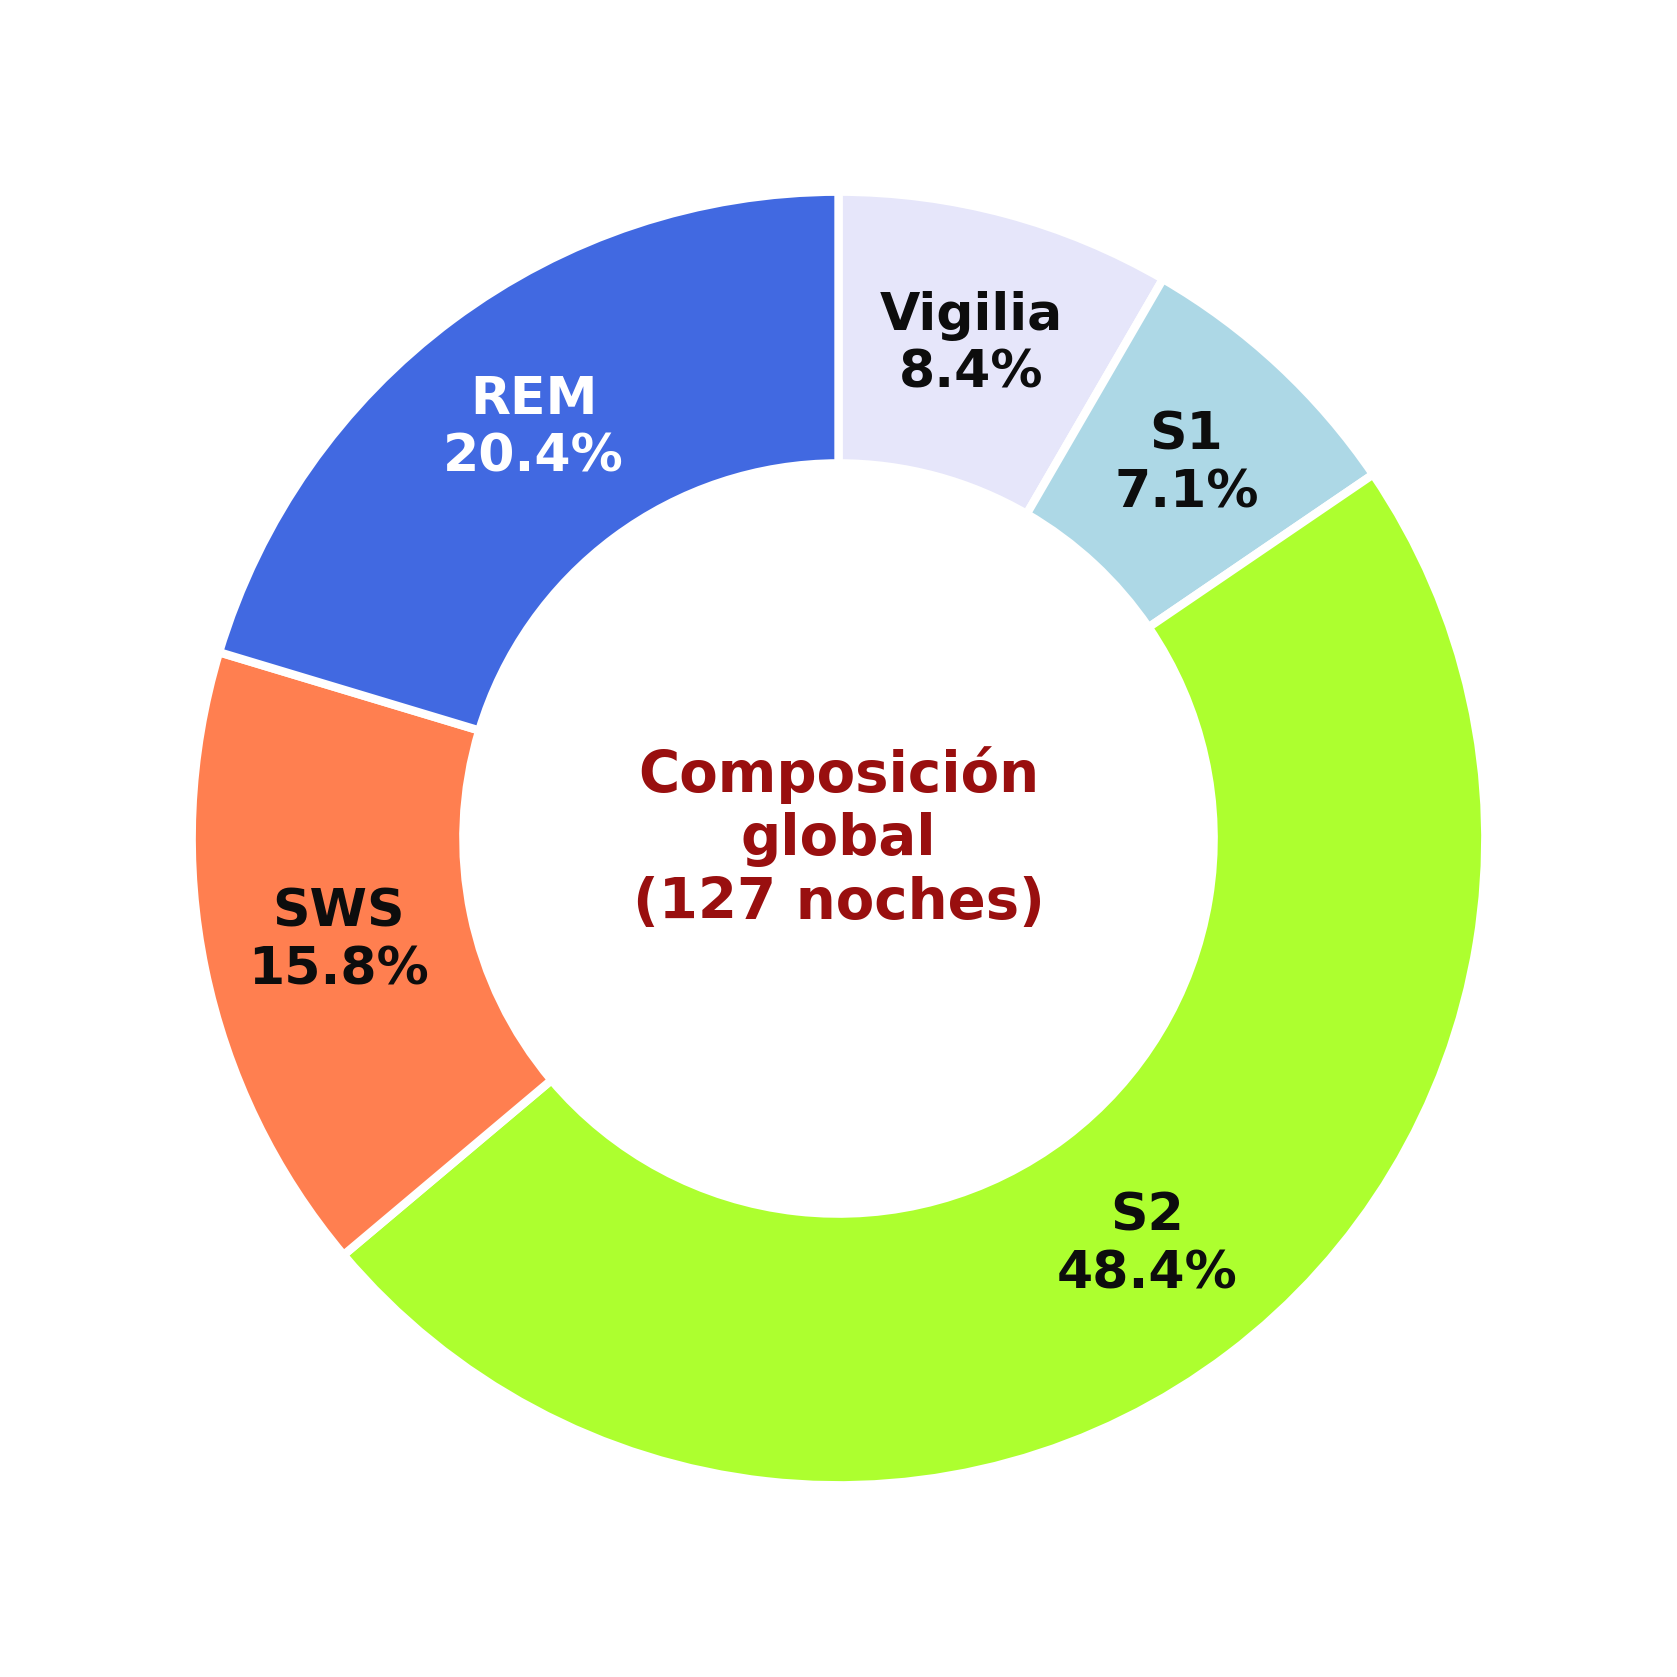
\includegraphics[width=\textwidth]{intro_estatico_donut.png}
        \caption{Enfoque Estático: Porcentajes globales.}
        \label{fig:estatico}
    \end{subfigure}

    \vspace{0.6em}

    \begin{subfigure}[b]{0.92\textwidth}
        \centering
        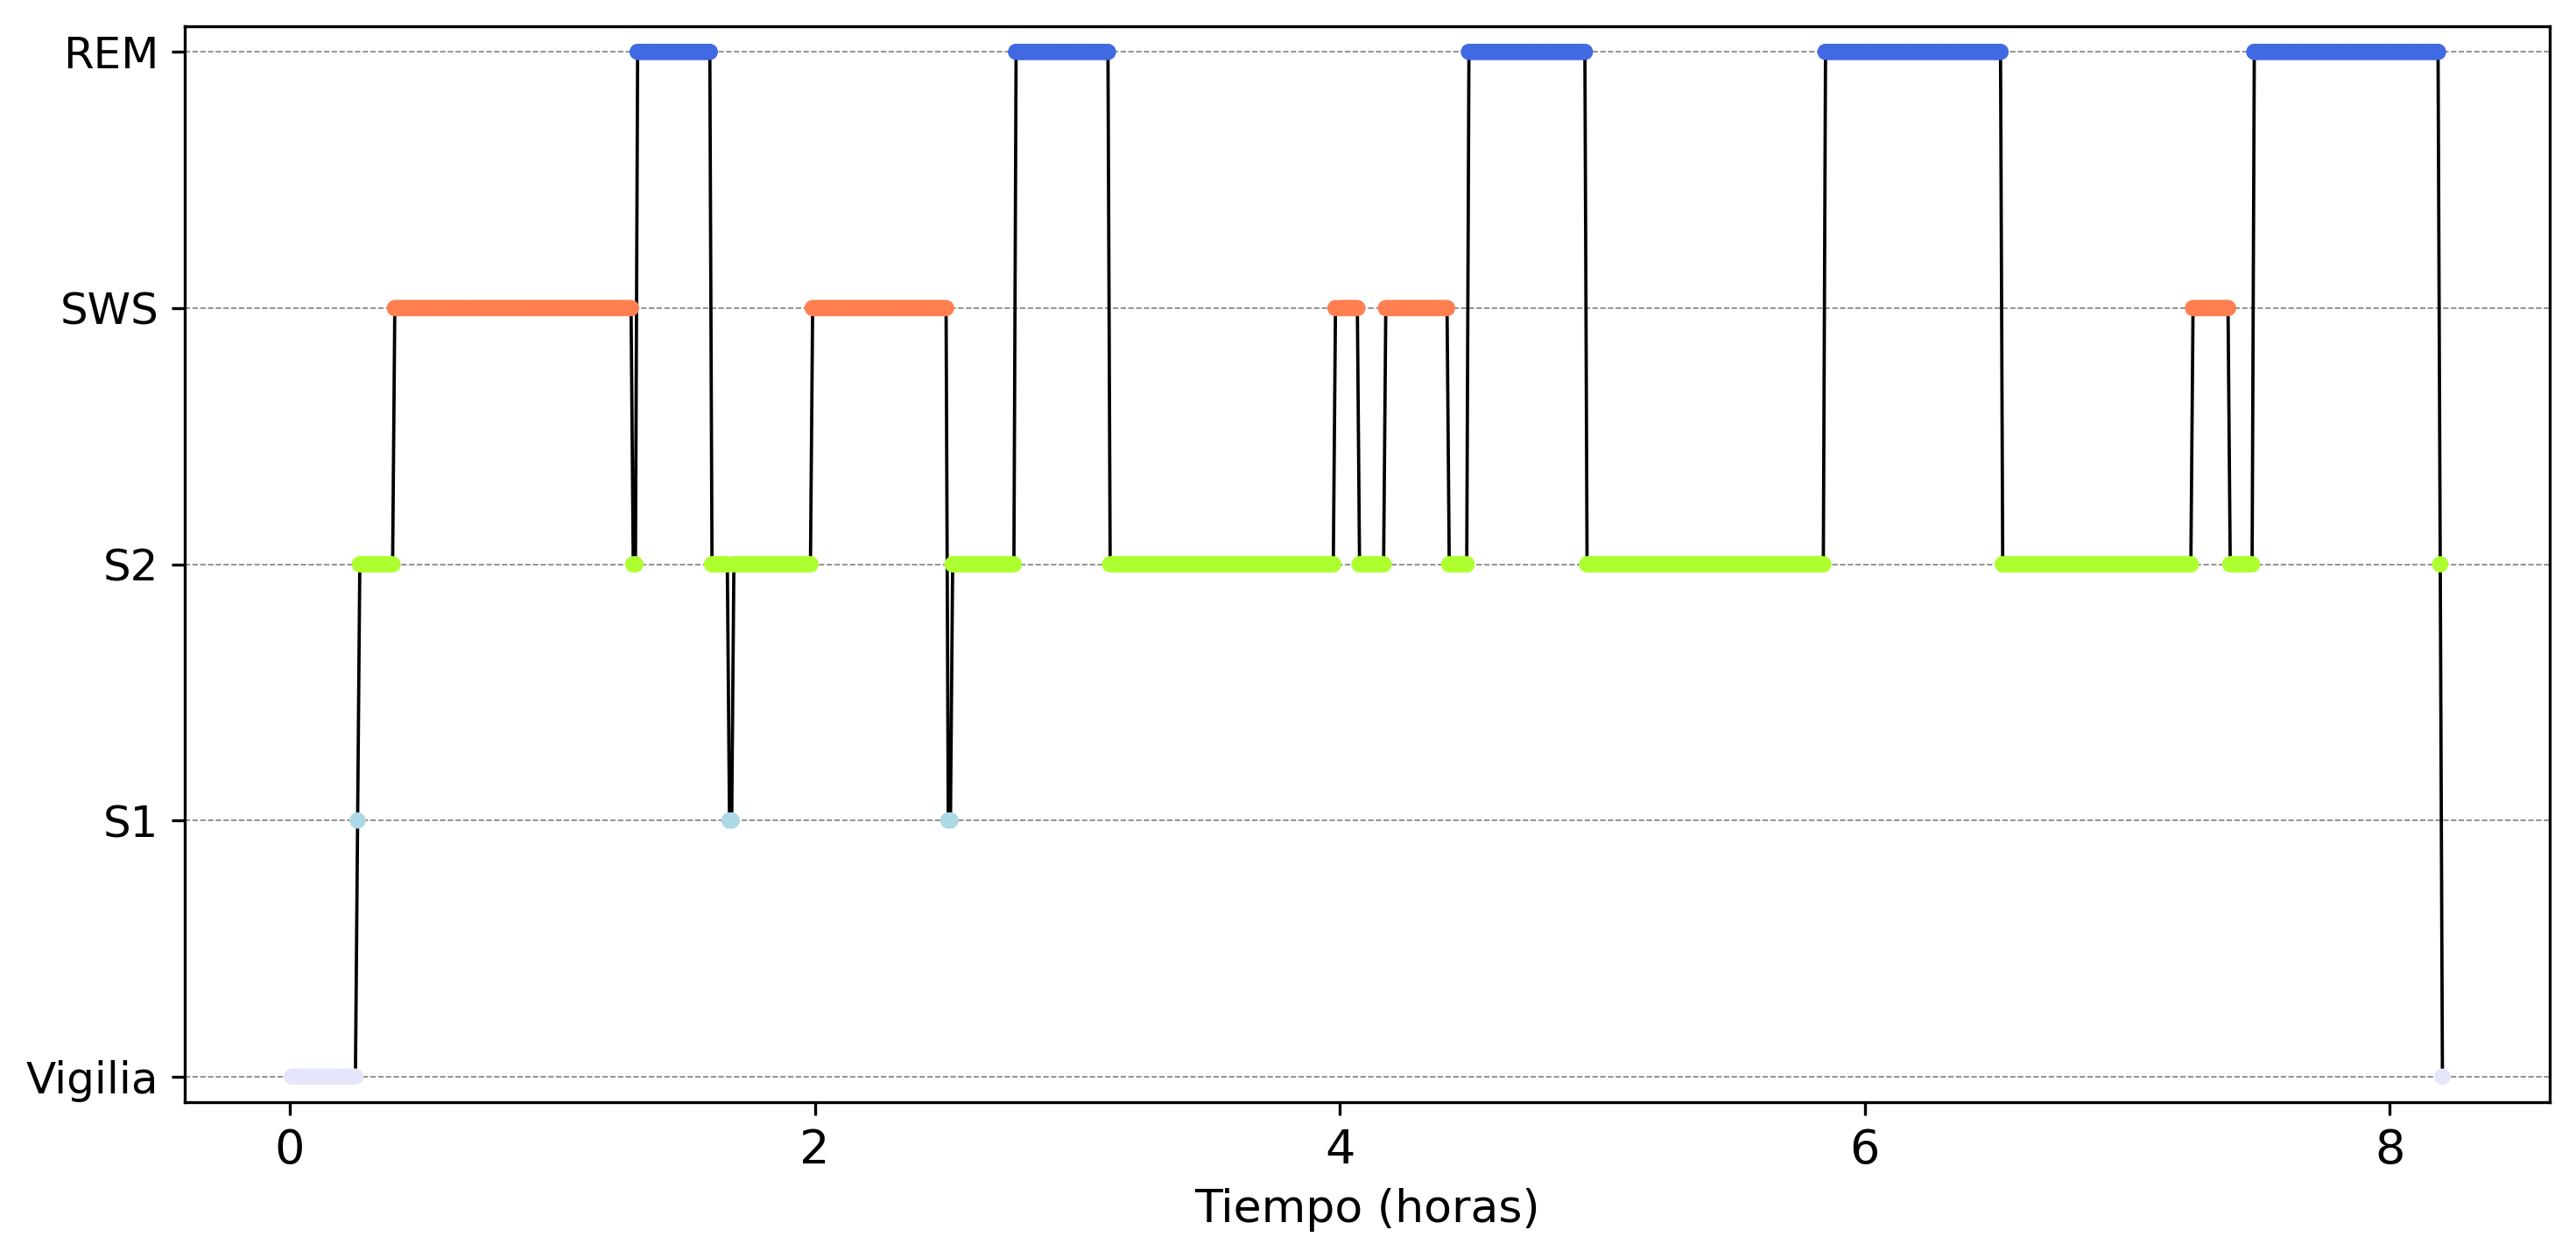
\includegraphics[width=\textwidth]{intro_dinamico_hipno.png}
        \caption{Enfoque Dinámico: Trayectoria secuencial.}
        \label{fig:dinamico}
    \end{subfigure}
    \caption{El Paradigma Estático vs. Dinámico. (A) Las métricas globales (porcentajes) ocultan la estructura temporal. (B) El análisis secuencial revela la intencionalidad y trayectoria de las transiciones.}
    \label{fig:problema_conceptual}
\end{figure}

Al reducir la complejidad del hipnograma a promedios globales, se pierde información crítica sobre la \textbf{intencionalidad} de las transiciones. Actualmente, no existen herramientas estandarizadas que permitan diferenciar si una época de S2 es un estado de ``profundización'' (preparándose para entrar a SWS) o un estado de ``activación'' (preparándose para REM). Esta ceguera metodológica impide comprender alteraciones sutiles en la arquitectura del sueño que no afectan los porcentajes totales, pero sí la continuidad y funcionalidad del ciclo.

\section{Justificación de la Investigación}

Esta investigación se justifica por la necesidad de incorporar herramientas modernas de \textbf{Inteligencia Artificial Interpretativa} al análisis de señales biomédicas. Mientras que el estado del arte en Deep Learning se ha enfocado en la clasificación automática (``cajas negras''), esta tesis propone un cambio de paradigma hacia el análisis de la dinámica.

Nuestros análisis (ver Capítulo \ref{resultados}) revelaron que la duración de los bloques de Fase 2 no sigue una distribución normal, sino una \textbf{distribución de cola pesada}, en la que la media (12.10 épocas) y la mediana (5 épocas) divergen marcadamente. Esto implica que no existe una ``duración promedio'' representativa y que los métodos estadísticos tradicionales (basados en la media y desviación estándar) resultan inadecuados.
La aplicación de técnicas de \textbf{Procesamiento de Lenguaje Natural (NLP)}, específicamente modelos de Embeddings, permite superar esta limitación. Al tratar las fases del sueño como ``palabras'' y los ciclos como ``oraciones'', podemos interrogar la estructura gramatical latente del hipnograma, abriendo la puerta a nuevos biomarcadores digitales basados en la trayectoria y no solo en la cantidad de sueño.

Finalmente, la relevancia clínica de esta propuesta radica en su potencial como \textbf{biomarcador temprano}. Muchas patologías del sueño y neurodegenerativas alteran la micro-arquitectura del sueño antes de que los porcentajes globales (el hipnograma macroscópico) muestren cambios evidentes. Si nuestra hipótesis es correcta y la Fase 2 posee subtipos funcionales, la pérdida de esta diferenciación dinámica podría servir como una señal de alerta precoz de fragmentación del sueño, invisible para las métricas actuales.

\section{Preguntas de Investigación e Hipótesis}

\subsection*{Interrogantes de Investigación}

\begin{enumerate}
    \item ¿Existe información en la estructura secuencial de los hipnogramas que permita caracterizar la dinámica del sueño (S2, SWS, REM) en los distintos ciclos de sueño?
    \item ¿Pueden los hipnogramas tratarse como secuencias simbólicas que, al segmentarse en unidades de varias épocas, exhiben las regularidades estadísticas propias de un lenguaje natural?
    \item ¿Es posible anticipar su transición a otras fases (SWS o REM) a partir de los vectores de incrustación?
\end{enumerate}

\subsection*{Hipótesis}

\begin{itemize}
    \item \textbf{H1 (Estructural):} El sueño de un participante sano no es un proceso aleatorio; sigue una estructura particular no fragmentada.
    \item \textbf{H2 (Lingüística):} Los hipnogramas son secuencias simbólicas que pueden ser tratadas mediante principios homólogos a los de un lenguaje natural.
    \item \textbf{H3 (Dinámica):} La representación vectorial de la Fase 2 presenta una bifurcación topológica en el espacio latente que correlaciona con su destino (SWS vs. REM), permitiendo anticipar la transición antes de que ocurra clínicamente.
\end{itemize}

\section{Objetivos}

\textbf{Objetivo General:}
Modelar la dinámica de las transiciones de sueño mediante un enfoque híbrido de Cadenas de Markov y algoritmos de Embeddings (Word2Vec), para caracterizar la heterogeneidad funcional de la Fase 2.

\textbf{Objetivos Específicos:}
\begin{enumerate}
    \item Cuantificar la estabilidad y las probabilidades de transición explícitas entre fases utilizando Matrices de Markov, diferenciando por ciclos de sueño para respetar la no-estacionariedad.
    \item Determinar la escala temporal de tokenización a la que las secuencias del hipnograma reproducen las regularidades estadísticas de un lenguaje natural, mediante un criterio multi-objetivo basado en la ley de Zipf.
    \item Entrenar un modelo de representación vectorial (Word2Vec Skip-Gram) sobre secuencias de hipnogramas para capturar las dependencias contextuales de largo plazo.
    \item Implementar técnicas de reducción de dimensionalidad (UMAP) y métricas de similitud coseno para visualizar y medir la trayectoria dinámica de la Fase 2 en el espacio latente.
    \item Validar si existe una ``bifurcación'' en la trayectoria de la Fase 2 que anticipe la entrada a estados de sueño profundo o REM.
\end{enumerate}

\section{Alcance y Delimitaciones}

El núcleo metodológico de este estudio se construye sobre hipnogramas de adultos sanos, que definen una referencia normativa de la arquitectura del sueño a partir de la cual se modela su dinámica. Metodológicamente, la resolución temporal del análisis ($N=6$ épocas) se fija mediante un criterio multi-objetivo que combina el ajuste a la ley de Zipf, la calidad de dicho ajuste y la cobertura de los bloques de Fase 2, sin recurrir a la calibración por un ciclo particular.

\FloatBarrier
\section{Estructura de la Tesis}

El presente trabajo se organiza en cinco capítulos:
\begin{itemize}
    \item \textbf{Capítulo 1: Introducción.} Presenta el contexto, la problemática y los objetivos del estudio.
    \item \textbf{Capítulo 2: Marco Teórico.} Revisa la fisiología del sueño, las limitaciones de los modelos estocásticos clásicos y fundamenta el uso de algoritmos de NLP y Manifold Learning.
    \item \textbf{Capítulo 3: Metodología.} Describe el procesamiento de datos, la configuración del modelo Word2Vec y los parámetros de visualización con UMAP.
    \item \textbf{Capítulo 4: Resultados.} Expone los hallazgos sobre la estabilidad markoviana y presenta las proyecciones vectoriales que evidencian la dinámica de la Fase 2.
    \item \textbf{Capítulo 5: Discusión y Conclusiones.} Interpreta los resultados a la luz de la fisiología del sueño, discute las implicaciones clínicas y propone líneas de trabajo futuro.
\end{itemize}

\chapter{Marco Teórico}
\chaptermark{Marco}
\label{marcoteo}

\section{Antecedentes y Estado del Arte}

El análisis computacional de la arquitectura del sueño ha evolucionado drásticamente, transitando desde modelos estocásticos clásicos hasta las arquitecturas de aprendizaje profundo (Deep Learning) que definen el estado del arte actual. Para situar nuestra contribución, revisamos la evolución de estos paradigmas y sus limitaciones para modelar la dinámica continua.

\subsection{Enfoques Estocásticos y Dinámica Simbólica}
El modelado matemático del sueño se remonta a los trabajos seminales de \cite{yang1973markov} y \cite{kemp1986analysis}, quienes establecieron que las transiciones entre fases no son aleatorias, sino que siguen una estructura markoviana.
Sin embargo, estos modelos clásicos enfrentan una limitación teórica fundamental: la \textbf{Propiedad de Falta de Memoria}. Al asumir distribuciones de permanencia geométricas, fallan en capturar la micro-arquitectura del sueño, donde la duración de las fases (especialmente la Fase 2) exhibe un comportamiento de cola pesada o invariante de escala, inconsistente con la caída exponencial de Markov.

Paralelamente, investigadores exploraron la \textbf{Dinámica Simbólica} y medidas de complejidad (como la Entropía de Shannon o Lempel-Ziv) para cuantificar la fragmentación del sueño \cite{bianchi2010probabilistic}. Aunque estos enfoques trataban al hipnograma como una secuencia de símbolos (precursores conceptuales de nuestro enfoque lingüístico), carecían de la capacidad de representación vectorial para capturar la semántica contextual de las transiciones.

Intentos posteriores, como los \textbf{Modelos Ocultos de Markov (HMM)} de \cite{flexer2002continuous}, introdujeron ``estados latentes'' para mitigar la rigidez de Markov, pero su dependencia de distribuciones de duración fijas y su complejidad computacional limitaron su adopción frente a métodos más modernos.

\subsection{La Hegemonía del Deep Learning: Clasificación vs. Interpretación}
Desde 2017, el campo ha sido dominado por el aprendizaje profundo, enfocado casi exclusivamente en la tarea de \textbf{Clasificación Automática (Sleep Staging)} para maximizar la concordancia con expertos humanos (F1-Score).

\begin{itemize}
    \item \textbf{Modelos Discriminativos (CNNs):} Arquitecturas pioneras como \textbf{DeepSleepNet} \cite{supratak2017deepsleepnet} demostraron que las Redes Convolucionales podían extraer características invariantes directamente del EEG crudo, superando a los métodos de extracción manual.
    
    \item \textbf{Modelos de Secuencia a Secuencia (Seq2Seq):} Reconociendo la importancia del contexto temporal, modelos como \textbf{SeqSleepNet} \cite{phan2019seqsleepnet} y más recientemente \textbf{SleepTransformer} \cite{phan2022sleeptransformer}, han adaptado mecanismos de atención y Transformers para procesar secuencias completas (Many-to-Many).
\end{itemize}

Sin embargo, existe una brecha crítica en esta literatura: el objetivo de estos modelos es puramente \textit{discriminativo} (etiquetar correctamente). Aunque algunos estudios recientes analizan los ``ciclos de hipnodensidad'' (probabilidades de salida de la red) \cite{stephansen2018neural}, estos reflejan la incertidumbre del clasificador, no necesariamente la estructura semántica latente del proceso fisiológico.

\subsection{La Brecha Actual: Manifold Learning en Sueño}
Aunque técnicas de reducción de dimensionalidad como UMAP han comenzado a aparecer en estudios recientes (2023-2025) \cite{deng2024umap}, la inmensa mayoría las utiliza como paso intermedio para mejorar la separabilidad de clases (clustering) y el diagnóstico automático.

Hasta la fecha, existe una ausencia notable de investigaciones que combinen \textbf{Embeddings Contextuales (Word2Vec)} con \textbf{Manifold Learning} para trazar la \textit{trayectoria dinámica} de la Fase 2. Esta tesis aborda este vacío, proponiendo que la geometría del espacio vectorial puede revelar estados de preparación anticipatoria (pre-SWS o pre-REM) invisibles para los clasificadores tradicionales y los modelos de hipnodensidad.

\section{Fisiología del Sueño y Polisomnografía}

El sueño es un proceso biológico activo, cíclico y altamente organizado, fundamental para la homeostasis del organismo. Lejos de ser una simple desconexión pasiva del entorno, el cerebro dormido exhibe patrones complejos de actividad eléctrica que regulan funciones críticas como la consolidación de la memoria, la restauración metabólica y la regulación emocional. Para el propósito de esta tesis, que busca modelar la dinámica de las transiciones de sueño mediante herramientas computacionales, es imperativo comprender primero la estructura biológica subyacente que estos modelos intentan capturar.

El estándar de oro para el estudio científico del sueño es la Polisomnografía (PSG). Este registro simultáneo de múltiples variables fisiológicas permite visualizar la arquitectura del sueño en tiempo real. Siguiendo los lineamientos clásicos establecidos en el manual de \cite{rechtschaffen1968manual}, las señales mínimas requeridas para una estadificación confiable incluyen:
\begin{itemize}
    \item \textbf{Electroencefalograma (EEG):} Registra la actividad eléctrica cortical. Es la señal principal para diferenciar las fases basándose en la frecuencia y amplitud de las ondas cerebrales (ritmos alfa, theta, delta, husos de sueño).
    \item \textbf{Electrooculograma (EOG):} Registra los movimientos oculares. Es crucial para identificar el inicio del sueño (movimientos oculares lentos en S1) y la fase REM (movimientos oculares rápidos).
    \item \textbf{Electromiograma (EMG):} Registra el tono muscular (generalmente mentoniano). Es indispensable para distinguir el sueño REM (atonía muscular) de la vigilia o fases ligeras.
\end{itemize}

\section{Estadificación del Sueño: Criterios de Rechtschaffen y Kales}

La clasificación de los estados de sueño se realiza tradicionalmente dividiendo el registro continuo en épocas (ventanas) de 30 segundos. A cada época se le asigna una etiqueta única basada en los patrones predominantes. A continuación, describimos las fases según los criterios de \cite{rechtschaffen1968manual}, enfatizando su relevancia para la dinámica de transiciones estudiada en este trabajo.

\subsection{Vigilia (W)}

El estado de vigilia con ojos cerrados se caracteriza por la presencia de un ritmo alfa dominante (8-13 Hz) en las regiones occipitales, acompañado de un tono muscular (EMG) elevado y movimientos oculares voluntarios o parpadeo. En el contexto de las transiciones, la vigilia representa el estado de ``retorno'' o fragmentación cuando aparece en mitad de la noche.

\subsection{Sueño No REM (NREM)}

El sueño NREM constituye aproximadamente el 75-80\% del sueño total en adultos y se subdivide en fases de profundidad progresiva. Desde la perspectiva de nuestros modelos vectoriales, el sueño NREM representa un continuo de actividad sincronizada.

\subsubsection{Fase 1 (S1)}

Es la etapa de transición entre la vigilia y el sueño. Se caracteriza por la desaparición del ritmo alfa y la aparición de ondas de bajo voltaje y frecuencia mixta (principalmente theta, 4-7 Hz). Fisiológicamente, es un estado inestable y breve (2-5\% de la noche). En nuestros análisis de grafos y matrices de transición, S1 actúa frecuentemente como un nodo de paso obligado desde la vigilia, pero raramente como un estado destino estable.

\subsubsection{Fase 2 (S2)}

Esta es la fase central de nuestra investigación. Representa entre el 45\% y el 55\% del tiempo total de sueño, convirtiéndola en el estado más abundante. Se define inequívocamente por la aparición de dos marcadores gráficos específicos sobre un fondo de actividad theta:
\begin{itemize}
    \item \textbf{Husos de Sueño (Sleep Spindles):} Ráfagas de actividad rítmica de 12-14 Hz que duran al menos 0.5 segundos. Se asocian con la inhibición del procesamiento sensorial (protección del sueño) y la consolidación de la memoria.
    \item \textbf{Complejos K:} Ondas lentas bifásicas de gran amplitud (>75 $\mu$V) que pueden ocurrir espontáneamente o como respuesta a estímulos externos.
\end{itemize}

La Figura \ref{fig:eeg_s2} ilustra estos elementos característicos del EEG durante la Fase 2.

\begin{figure}[htbp]
    \centering
    \includegraphics[width=0.75\textwidth]{Stage 2 sleep EEG K complex Sleep Spindle.png}
    \caption{Elementos característicos del EEG en Fase 2. (A) Huso de Sueño: ráfaga de actividad sigma (12-14 Hz). (B) Complejo K: onda bifásica de gran amplitud.}
    \label{fig:eeg_s2}
\end{figure}

Tradicionalmente, S2 se ha considerado una fase de ``transición'' o mantenimiento. Sin embargo, nuestra hipótesis de ``memoria latente'' sugiere que la S2 no es homogénea. Aunque visualmente idéntica según R\&K, proponemos que la micro-estructura de S2 varía funcionalmente dependiendo de si el cerebro se está ``preparando'' para profundizar hacia SWS o para activarse hacia REM.

\paragraph*{Limitaciones del Estándar Visual.}
Es crucial notar que el sistema R\&K es una discretización macroscópica (ventanas de 30s) que asume homogeneidad dentro de la etiqueta. Sin embargo, este estándar ignora la micro-estructura y la dinámica continua de la señal EEG. Al reducir 30 segundos de actividad eléctrica compleja a un solo número entero (el ``token''), se pierde información sobre la evolución interna del estado. Los modelos de embeddings vectoriales propuestos en este trabajo buscan recuperar esa ``información oculta'' latente en la secuencialidad, que el ojo humano y las reglas estrictas de R\&K no pueden capturar explícitamente.

\subsubsection{Sueño de Ondas Lentas (SWS)}

Corresponde al sueño profundo. \cite{rechtschaffen1968manual} distinguían entre S3 (20-50\% de ondas delta) y S4 (>50\% de ondas delta). En la práctica moderna y en este trabajo, ambas se unifican bajo la etiqueta SWS (Slow Wave Sleep). Se caracteriza por ondas delta de gran amplitud (>75 $\mu$V) y baja frecuencia (0.5-2 Hz). Es la fase de mayor umbral para el despertar y está fuertemente regulada por la presión homeostática: es predominante en el primer tercio de la noche y disminuye exponencialmente en los ciclos subsiguientes. Esta dinámica temporal es la que justifica nuestro enfoque de analizar el ``Primer Ciclo'' por separado para calibrar la escala temporal de los embeddings.

\subsection{Sueño REM (Movimientos Oculares Rápidos)}

El sueño REM es un estado paradójico: el EEG muestra una actividad desincronizada de bajo voltaje y frecuencia mixta, muy similar a la vigilia o la fase S1 (``dientes de sierra''), pero el cuerpo se encuentra en una parálisis muscular completa (atonía en el EMG). Se acompaña de ráfagas de movimientos oculares rápidos.

El REM es el estado donde ocurren los sueños vívidos más narrativos. En la arquitectura del sueño, el REM y el SWS actúan como polos opuestos de un ciclo ultradiano. La transición de S2 a REM es, según nuestros resultados vectoriales, un ``salto'' semántico abrupto, a diferencia de la transición suave hacia SWS.

\section{Analogía Lingüística y Semántica Distribucional del Sueño}

Si bien el sueño es un proceso fisiológico, su representación mediante hipnogramas (secuencias discretas de símbolos) permite analizarlo bajo la óptica de la Teoría de la Información y la Lingüística Computacional. Al igual que el lenguaje natural, el sueño posee una \textbf{sintaxis} (reglas probabilísticas de transición, p.ej., S1 $\rightarrow$ S2 es gramaticalmente correcto, REM $\rightarrow$ SWS es agramatical o raro) y una \textbf{semántica} (el significado funcional de una fase depende de su contexto).

Esta tesis se fundamenta en la \textbf{Hipótesis Distribucional}, la cual postula que elementos con contextos similares poseen significados similares. Para capturar esta semántica, utilizamos la arquitectura \textit{Skip-Gram} (ver Figura \ref{fig:skipgram}). A diferencia de los modelos clásicos, esta red neuronal toma la fase actual (por ejemplo, una época de S2) como entrada e intenta predecir las fases que la rodean (su contexto pasado y futuro). De esta forma, el vector resultante aprende a codificar no solo qué fase es, sino qué función cumple dentro de la secuencia.

\begin{figure}[htbp]
    \centering
    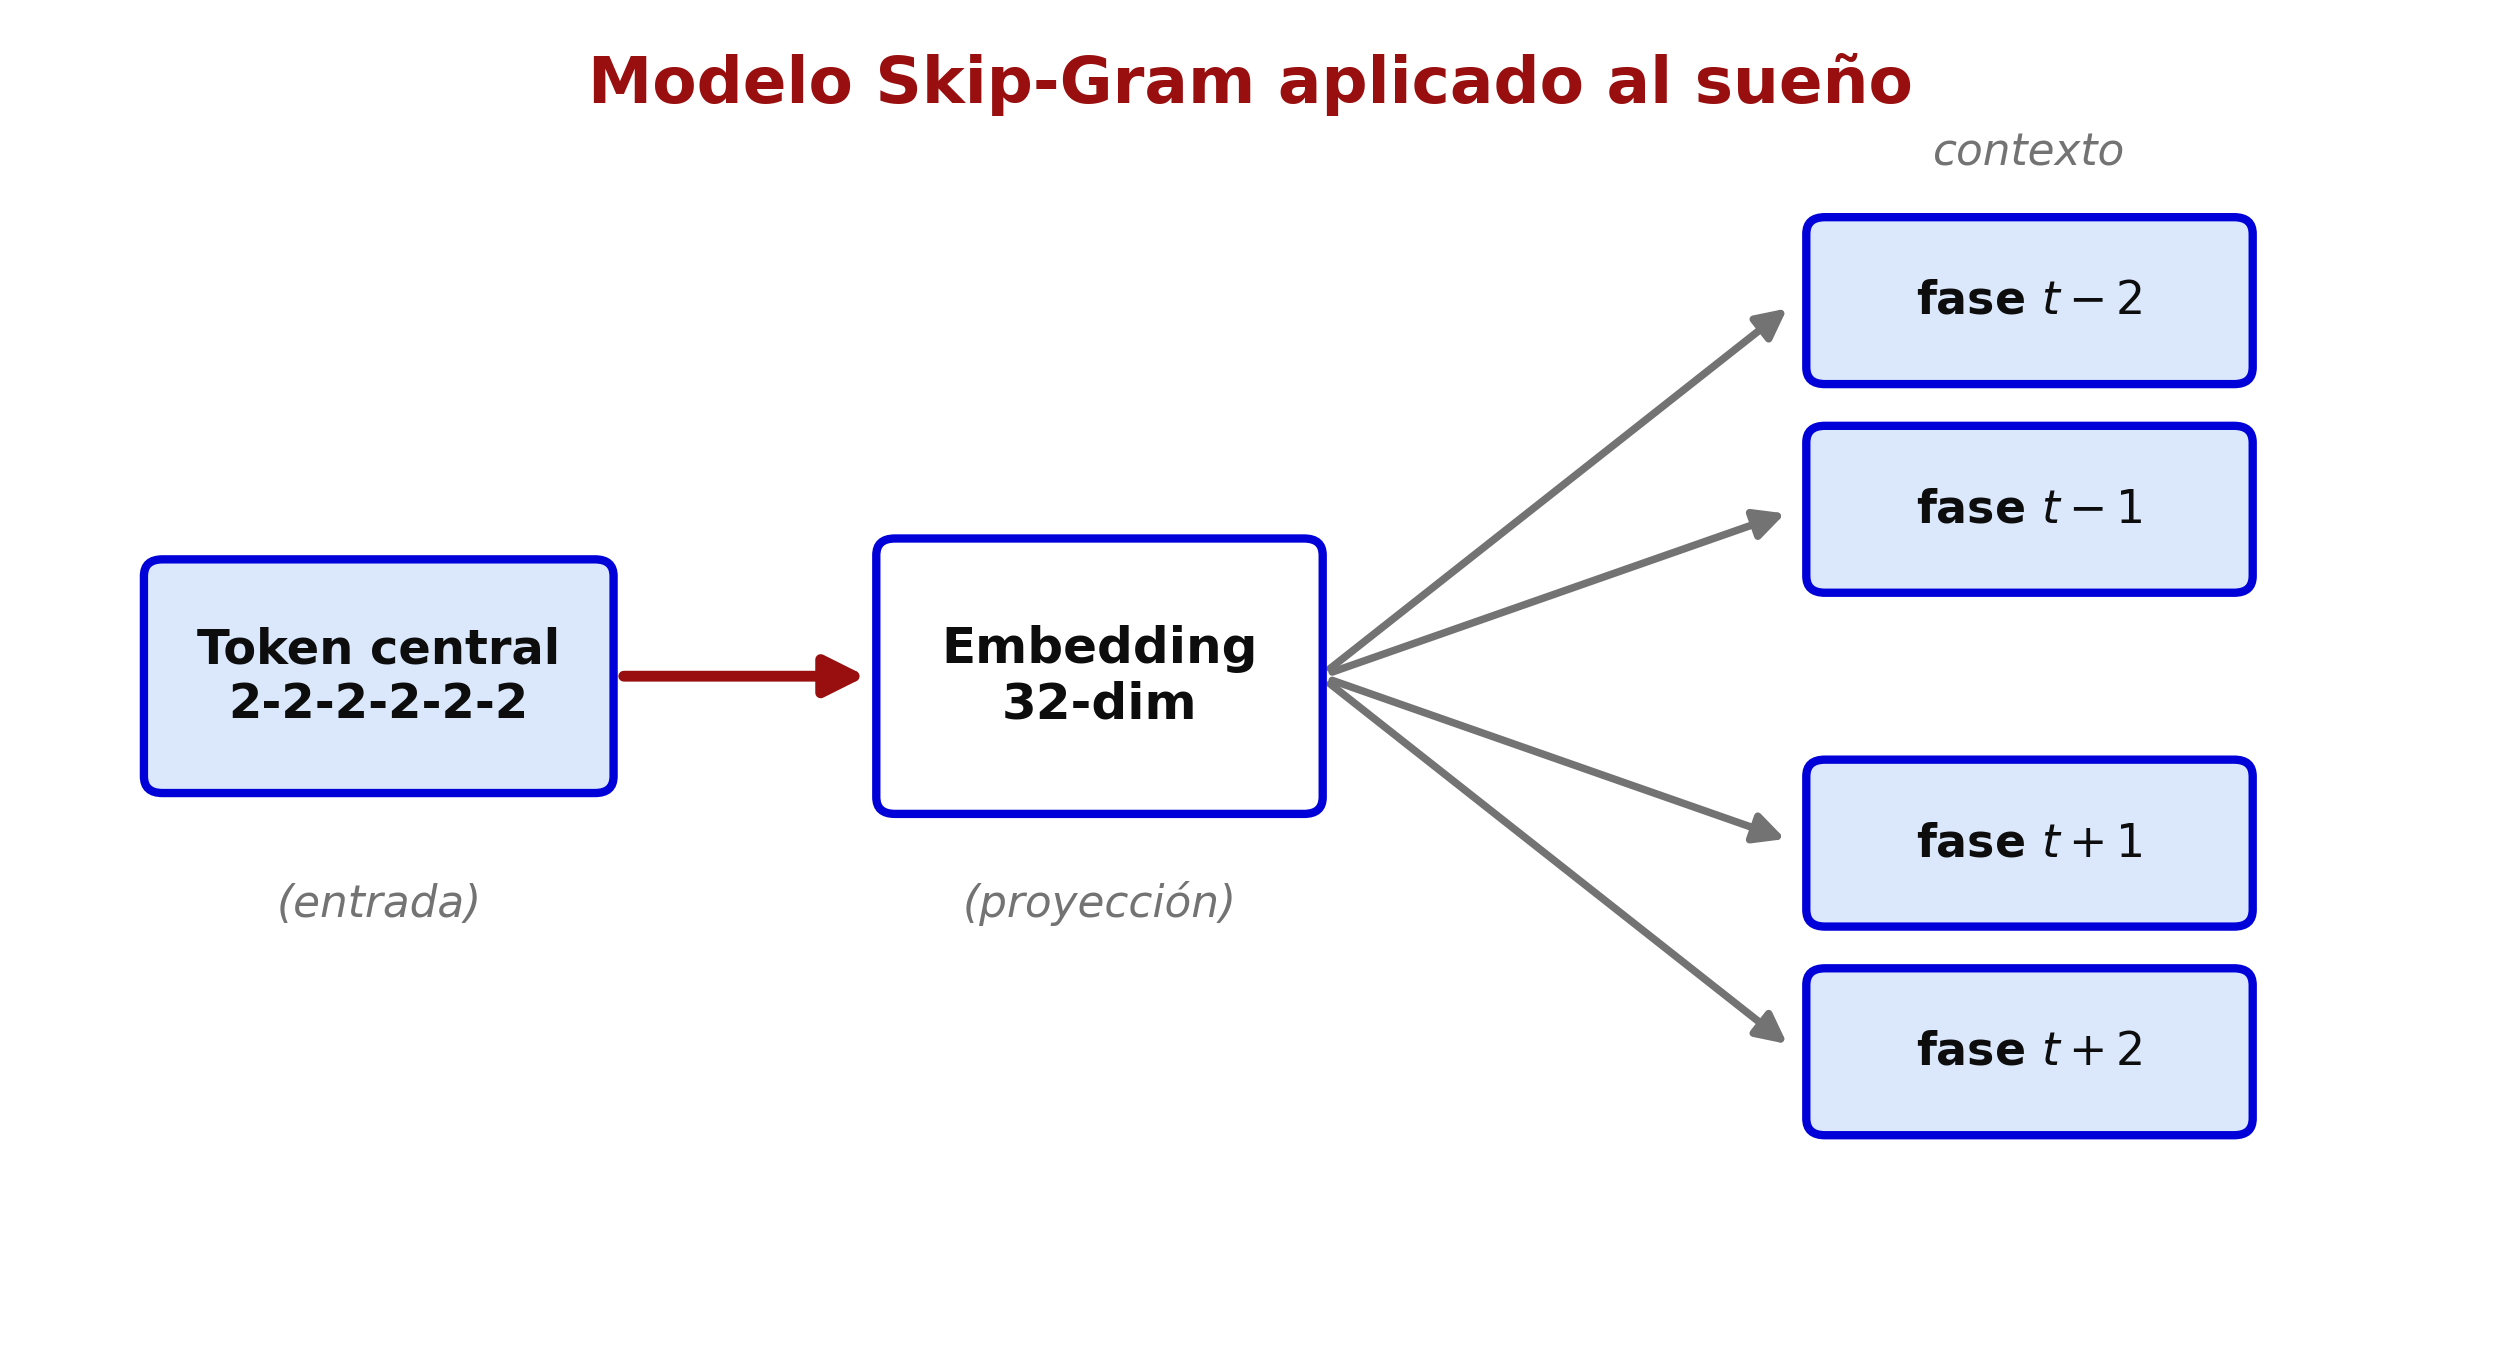
\includegraphics[width=0.95\textwidth]{skipgram_sueno.png}
    \caption{Arquitectura del modelo Skip-Gram aplicada al sueño. El nodo central representa la fase actual (Input) y la red optimiza los pesos para predecir las fases vecinas (Output), capturando así la dinámica de transición.}
    \label{fig:skipgram}
\end{figure}

En nuestro marco, asumimos que una época de S2 que precede al sueño profundo (contexto de profundización) posee una ``carga semántica'' distinta a una época de S2 que precede al REM (contexto de activación), aunque ambas compartan la misma etiqueta en la clasificación macroscópica de R\&K.

\section{Ciclos de Sueño y Dinámica Temporal}

El sueño no ocurre en bloques aislados, sino que se organiza en ciclos ultradianos de aproximadamente 90 a 110 minutos, alternando entre sueño NREM y REM. Como se ilustra en la Figura \ref{fig:hipnograma}, la arquitectura del sueño no es uniforme: el sueño profundo (SWS) se concentra predominantemente en el primer tercio de la noche, mientras que la fase REM se vuelve más frecuente y prolongada en los ciclos tardíos.

\begin{figure}[htbp]
    \centering
    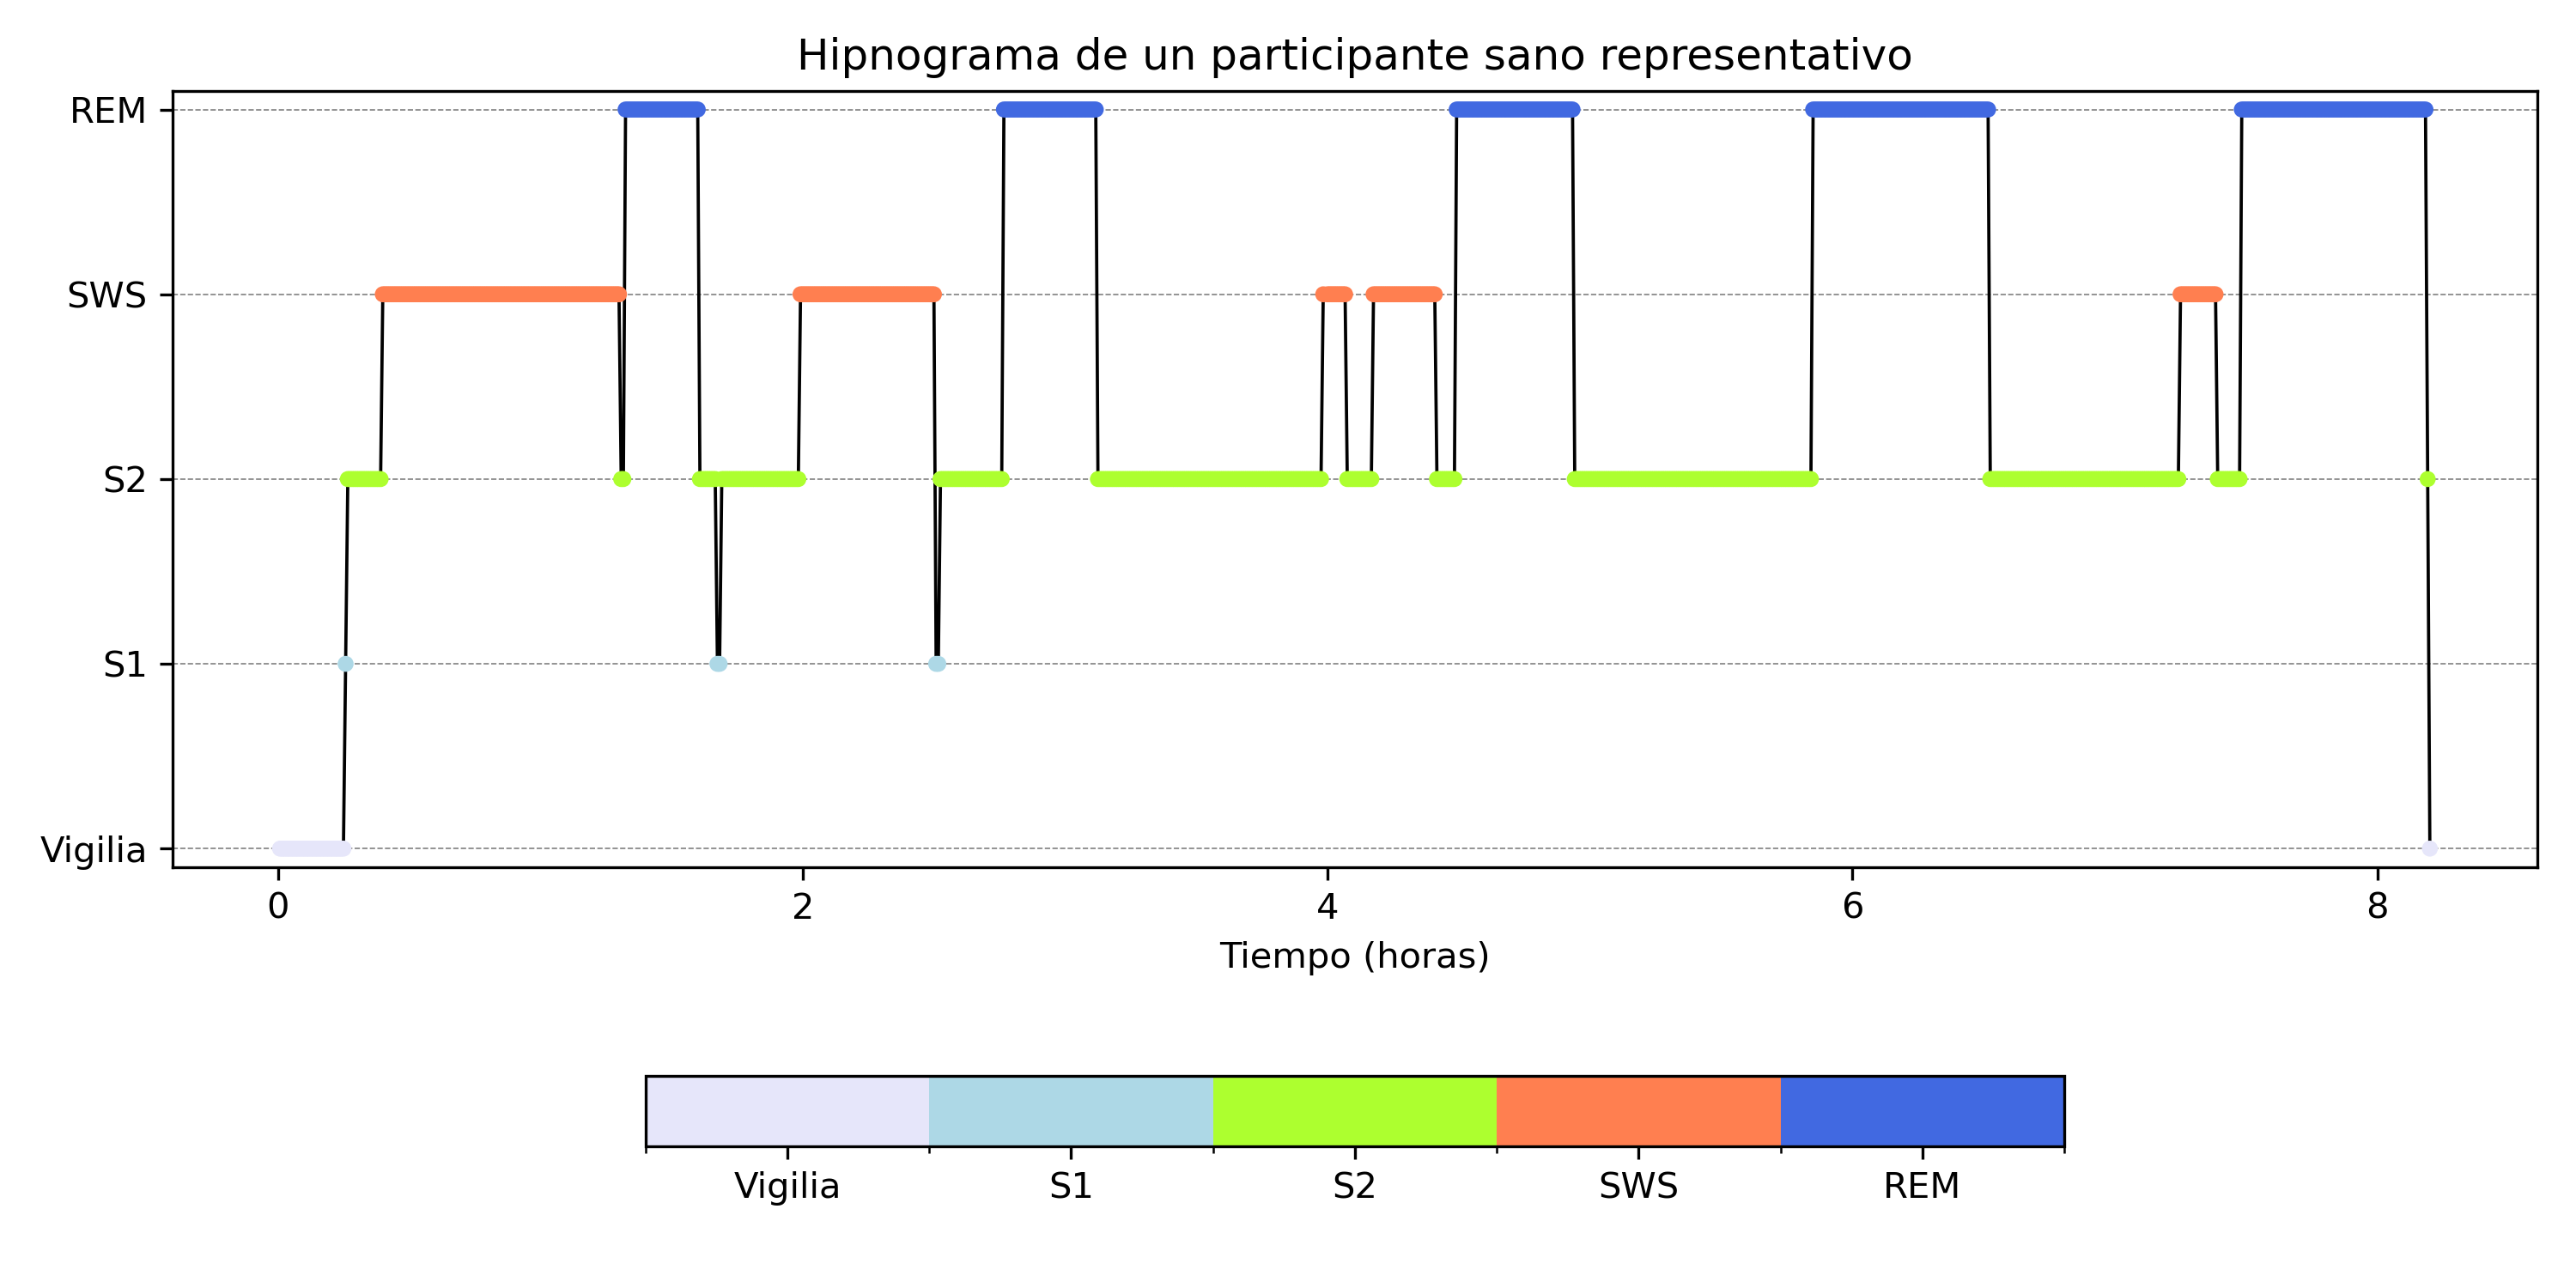
\includegraphics[width=0.95\textwidth]{hipnograma_modelo.png}
    \caption{Hipnograma de un participante sano representativo del conjunto de datos unificado. Nótese la predominancia de Sueño Profundo (SWS) en el primer tercio de la noche y el aumento progresivo del REM en los ciclos subsiguientes, ilustrando la no-estacionariedad del proceso.}
    \label{fig:hipnograma}
\end{figure}

Desde una perspectiva estocástica, la arquitectura del sueño ha sido frecuentemente modelada como una Cadena de Markov. Sin embargo, una asunción crítica de los modelos markovianos simples es la \textbf{estacionariedad} (que las probabilidades de transición son constantes en el tiempo). La evidencia fisiológica (Modelo de Borbély) sugiere que el sueño es intrínsecamente \textbf{no-estacionario}: la probabilidad de pasar de S2 a SWS es alta al inicio de la noche (presión homeostática alta) y casi nula al final (presión disipada). Reconocer esta no-estacionariedad es fundamental para nuestra metodología, justificando el uso de ventanas deslizantes y análisis segmentado por ciclos en lugar de métricas globales que promediarían comportamientos dinámicos opuestos.

\begin{itemize}
    \item \textbf{Primer Ciclo:} Predomina el SWS y el REM es corto o inexistente. Aquí la presión homeostática es máxima, lo que genera estructuras de sueño más estables y consolidadas.
    \item \textbf{Ciclos Tardíos:} A medida que la presión de sueño se disipa, el SWS desaparece y los periodos REM se alargan y fragmentan.
\end{itemize}

\section{Regulación del Sueño y Factores Experimentales}

Para comprender la dinámica temporal descrita anteriormente y justificar la selección de nuestros datos, es necesario recurrir a dos conceptos teóricos fundamentales.

\subsection{El Modelo de los Dos Procesos (Borbély)}

Propuesto por \citet{borbely1982two}, este modelo postula que la regulación del sueño es el resultado de la interacción entre dos procesos:
\begin{itemize}
    \item \textbf{Proceso S (Homeostático):} Representa la ``presión de sueño'' que se acumula durante la vigilia y se disipa exponencialmente durante el sueño, específicamente durante el SWS.
    \item \textbf{Proceso C (Circadiano):} Es un ritmo oscilatorio de aproximadamente 24 horas, independiente del sueño previo, que regula los umbrales de alerta y sueño.
\end{itemize}

La Figura \ref{fig:borbely} visualiza la interacción entre estos dos procesos.

\begin{figure}[htbp]
    \centering
    \includegraphics[width=0.9\textwidth]{Procesos.png}
    \caption{Modelo de los Dos Procesos de Borbély (1982). El Proceso S (Homeostático) muestra su máxima presión al inicio de la noche, lo que justifica teóricamente la mayor estabilidad estructural observada en el primer ciclo.}
    \label{fig:borbely}
\end{figure}

Este modelo proporciona el sustento teórico para nuestra decisión metodológica de analizar el \textbf{Primer Ciclo} por separado. Dado que el Proceso S es máximo al inicio de la noche, el primer ciclo presenta la estructura más robusta y menos fragmentada. Es en este periodo donde la duración de las fases (como S2) refleja su escala temporal ``natural'' antes de verse alterada por la disipación de la presión homeostática en ciclos posteriores.

\subsection{El Efecto de Primera Noche (First Night Effect)}

El ``Efecto de Primera Noche'' es un fenómeno bien documentado en la investigación del sueño, caracterizado por una alteración de la arquitectura del sueño (menor eficiencia, más despertares, latencias REM prolongadas) debido a la falta de adaptación del sujeto al entorno del laboratorio y a los sensores. Por esta razón, en esta investigación se descartaron sistemáticamente los registros de la primera noche, utilizando exclusivamente los datos de la \textbf{Noche 2}. Esto asegura que los patrones de transición y las estructuras vectoriales que analizamos correspondan a un sueño fisiológico basal y no a una respuesta de estrés adaptativo.

\section{Fundamentos Algorítmicos}

Para modelar la dinámica de las transiciones de sueño y extraer patrones ocultos en la secuencialidad de las fases, esta tesis emplea un enfoque híbrido que combina la teoría clásica de procesos estocásticos con técnicas modernas de aprendizaje de representaciones (Embeddings). A continuación, se detallan los fundamentos matemáticos de las Cadenas de Markov, herramienta base para nuestro análisis de estabilidad y transición.

\subsection{Modelado Estocástico: Cadenas de Markov}

Para entender cómo modelamos las transiciones entre fases, utilizamos el concepto de \textbf{Cadena de Markov}. Imaginemos el sueño no como una película continua, sino como una serie de fotografías tomadas cada 30 segundos (épocas). En cada foto, el cerebro está en un estado específico (por ejemplo, S2). La pregunta clave es: \textit{¿Qué probabilidad hay de que en la siguiente foto el cerebro cambie a REM o se quede en S2?}

Una Cadena de Markov es un modelo que asume que \textbf{el futuro inmediato depende solo del presente}. Es decir, para predecir si el paciente entrará en sueño profundo en el siguiente minuto, solo necesitamos saber en qué fase está \textit{ahora}, sin importar todo lo que pasó horas antes. A esta característica se le llama ``propiedad de falta de memoria''.

Matemáticamente, si $X_t$ es la fase del sueño en el tiempo actual $t$, la probabilidad de moverse a una fase futura $j$ dado que estamos en la fase $i$ se escribe como:

\begin{equation}
    P(X_{t+1} = j \mid X_t = i) = p_{ij}
\end{equation}

Todos estos posibles movimientos se organizan en una tabla llamada \textbf{Matriz de Transición} ($\mathbf{P}$). Es como un mapa de probabilidades que nos indica las rutas más frecuentes:

\begin{equation}
    \mathbf{P} = \begin{pmatrix}
    p_{11} & p_{12} & \dots & p_{1k} \\
    p_{21} & p_{22} & \dots & p_{2k} \\
    \vdots & \vdots & \ddots & \vdots \\
    p_{k1} & p_{k2} & \dots & p_{kk}
    \end{pmatrix}
\end{equation}

Cada fila de esta matriz representa el estado actual (``Desde dónde salgo'') y cada columna el estado futuro (``A dónde voy''). La suma de cada fila siempre es 1, porque el sistema obligatoriamente debe transicionar a algún estado en $t+1$.

Esta matriz admite una lectura como grafo dirigido: cada fase es un nodo y cada probabilidad de transición $p_{ij}$ una arista que lo conecta con el estado siguiente. Los valores de la diagonal ($p_{ii}$) corresponden a los bucles que un nodo dirige hacia sí mismo y reflejan la propiedad de inercia o permanencia en el estado.

Además, la estructura de la matriz revela dos propiedades críticas para nuestra investigación:
\begin{itemize}
    \item \textbf{Centralidad de S2:} La Fase 2 actúa como un ``Hub'' o distribuidor central, conectando el inicio del sueño con las fases profundas (SWS) y el REM.
    \item \textbf{Restricción Fisiológica:} La ausencia de una conexión directa SWS $\to$ REM confirma que el modelo respeta la sintaxis biológica del sueño sano.
\end{itemize}

\subsubsection{Estimación y Espacio de Estados}

Para la aplicación en arquitectura del sueño, definimos el espacio de estados $\mathcal{S}$ con las cinco fases fisiológicas del sueño:

\begin{equation}
    \mathcal{S} = \{0: \text{W}, 1: \text{S1}, 2: \text{S2}, 3: \text{SWS}, 4: \text{REM}\}
\end{equation}

Donde \textbf{SWS} (Slow Wave Sleep) unifica las etapas S3 y S4. Las épocas sin clasificar (movimiento o etiquetas ausentes, código 5) se tratan como ruido y se excluyen del cálculo de las matrices de transición.

Los parámetros de la matriz $\mathbf{P}$ se estiman a partir de los hipnogramas utilizando el \textbf{Estimador de Máxima Verosimilitud (MLE)}. Dado un conjunto de observaciones, la probabilidad estimada $\hat{p}_{ij}$ se calcula como la frecuencia relativa de las transiciones observadas:

\begin{equation}
    \hat{p}_{ij} = \frac{n_{ij}}{\sum_{k \in \mathcal{S}} n_{ik}}
\end{equation}

Donde $n_{ij}$ es el número total de veces que se observó una transición directa del estado $i$ al estado $j$.

\subsubsection{Implicaciones Teóricas: Inercia y Distribución de Permanencia}

Un componente crítico para nuestro análisis es la diagonal principal de la matriz ($p_{ii}$), que cuantifica la \textbf{inercia} o estabilidad del estado.

Desde la teoría de procesos estocásticos, la probabilidad de permanecer en un estado $i$ durante exactamente $k$ épocas consecutivas en una cadena de Markov sigue obligatoriamente una \textbf{Distribución Geométrica}:

\begin{equation}
    P(\text{Duración} = k) = (p_{ii})^{k-1} (1 - p_{ii})
\end{equation}

\textbf{Limitación Crítica:} Este modelo asume implícitamente que la probabilidad de abandonar una fase es constante en cada paso temporal (falta de memoria). Sin embargo, la evidencia biológica sugiere que la duración de fases como la N2 sigue distribuciones de cola larga (\textbf{Leyes de Potencia}) y no geométricas. Esta discrepancia teórica justifica la necesidad de incorporar modelos que capturen dependencias de largo plazo, como los embeddings vectoriales (Word2Vec), superando la visión ``sin memoria'' de Markov.

\subsubsection{No-Estacionariedad y Análisis por Ciclos}

Finalmente, es necesario abordar la \textbf{Estacionariedad}. Una cadena de Markov estándar asume que la matriz $\mathbf{P}$ es constante a lo largo del tiempo (homogénea en el tiempo).
No obstante, la regulación homeostática del sueño (Modelo de Borbély) implica que el proceso es \textbf{No-Estacionario}: la probabilidad de transitar a SWS ($p_{\text{S2} \to \text{SWS}}$) es alta al inicio de la noche y disminuye progresivamente.

Para modelar esta dinámica sin violar los supuestos matemáticos, en esta tesis adoptamos un enfoque de \textbf{Cadenas de Markov por Tramos (Piecewise Markov Chains)}, calculando una matriz de transición independiente $\mathbf{P}^{(c)}$ para cada ciclo de sueño $c$. Esto permite cuantificar matemáticamente la degradación de la estabilidad del sueño a medida que avanza la noche.

\subsection{Modelado Vectorial: Aprendizaje de Representaciones (Embeddings)}

Si las Cadenas de Markov nos permiten cuantificar la estabilidad y las transiciones inmediatas, los modelos de aprendizaje de representaciones nos permiten capturar el \textit{contexto} y las dependencias de largo plazo. En esta tesis, adaptamos técnicas de Procesamiento de Lenguaje Natural (NLP), específicamente el algoritmo \textbf{Word2Vec}, para modelar la dinámica secuencial del sueño.

\subsubsection{La Hipótesis Distribucional en el Sueño}

La base teórica de este enfoque es la \textbf{Hipótesis Distribucional} de \cite{harris1954distributional}, popularizada por Firth: \textit{``Conocerás a una palabra por la compañía que frecuenta''}. En lingüística, esto significa que palabras con contextos similares (ej. ``perro'' y ``gato'' aparecen cerca de ``ladrar'' o ``maullar'') tienen significados semánticos similares.

Transponiendo este concepto a la neurofisiología del sueño:
\begin{quote}
    \textit{La función de una fase de sueño no está definida solo por sus características espectrales intrínsecas (lo que ocurre en esos 30 segundos), sino por su posición en la secuencia temporal (de dónde viene y a dónde va).}
\end{quote}

Bajo esta premisa, una época de Fase 2 (S2) que precede al sueño profundo (SWS) es funcionalmente distinta de una época de S2 que precede al sueño REM, aunque para un experto humano se vean idénticas en el EEG. Nuestro objetivo es capturar esta diferencia latente mediante vectores matemáticos.

\subsubsection{Algoritmo Word2Vec (Skip-Gram)}

Utilizamos la arquitectura \textbf{Skip-Gram} de Word2Vec \cite{mikolov2013efficient, mikolov2013distributed}. A diferencia de otros modelos que usan el contexto para adivinar la palabra central (CBOW), Skip-Gram funciona al revés: toma una fase central y trata de predecir qué fases la rodean.

Por ejemplo, imaginemos una secuencia de sueño:
\[ \dots, \text{S1}, \text{S2}, \mathbf{S2}, \text{SWS}, \text{SWS}, \dots \]
Si nuestra ventana de contexto es $c=2$ y la fase central es la segunda \textbf{S2} ($w_t$), el modelo intentará maximizar la probabilidad de predecir sus vecinos: $P(\text{S1} \mid \text{S2})$, $P(\text{S2} \mid \text{S2})$, $P(\text{SWS} \mid \text{S2})$.

\paragraph*{Codificación y Definiciones}
Para que la red neuronal procese estos símbolos, cada fase $w$ se representa inicialmente como un vector \textbf{One-Hot} $x \in \{0,1\}^W$ (un vector lleno de ceros con un único 1 en la posición de la fase activa). Este vector de entrada se proyecta a un espacio latente de menor dimensión.

Formalmente, dado un hipnograma $w_1, w_2, \dots, w_T$, el objetivo es maximizar la probabilidad promedio:

\begin{equation}
    \frac{1}{T} \sum_{t=1}^{T} \sum_{-c \le j \le c, j \ne 0} \log P(w_{t+j} \mid w_t)
\end{equation}

Donde $v_w \in \mathbb{R}^D$ es la representación vectorial (embedding) de la fase, siendo $D$ la dimensión del espacio (un hiperparámetro elegido, ej. $D=32$). La probabilidad se calcula mediante la función Softmax sobre todo el vocabulario de tamaño $W$:

\begin{equation}
    P(w_O \mid w_I) = \frac{\exp({v'_{w_O}}^\top v_{w_I})}{\sum_{w=1}^{W} \exp({v'_w}^\top v_{w_I})}
\end{equation}

El resultado es un espacio vectorial donde la \textit{cercanía geométrica} (similitud coseno) refleja la \textit{similitud funcional}: si dos fases predicen los mismos vecinos, sus vectores serán similares.

\begin{quote}
    \textbf{Nota Técnica (Fases vs. N-gramas):} Aunque este ejemplo utiliza fases individuales como tokens para claridad expositiva, la misma lógica matemática aplica si los tokens son \textbf{N-gramas} (bloques de fases consecutivas). En esta tesis, utilizamos bloques de 6 épocas como tokens para capturar estructuras temporales de mayor escala, tal como se justifica a continuación.
\end{quote}

\subsubsection{Justificación Metodológica: De Leyes de Potencia a Vectores}

La decisión de utilizar embeddings no fue arbitraria, sino que surgió de una limitación fundamental de los métodos estadísticos clásicos observada en nuestros datos:

\begin{enumerate}
    \item \textbf{Invarianza de Escala (Leyes de Potencia):} Al analizar la distribución de duración de la Fase 2, descubrimos que no sigue una distribución normal (Campana de Gauss), sino una \textbf{Ley de Potencia} (Power Law). Esto implica que no existe una ``duración típica'' de la Fase 2; el cerebro genera eventos de S2 que pueden durar desde 30 segundos hasta 20 minutos.
    
    \item \textbf{El Problema de la Ventana Fija:} Debido a esta invarianza de escala, cualquier análisis basado en ventanas de tiempo fijas y arbitrarias (ej. ``analizar bloques de 5 minutos'') es metodológicamente incorrecto, ya que corta procesos fisiológicos de distinta magnitud.
    
    \item \textbf{Solución Vectorial:} Word2Vec resuelve este problema porque no impone una duración rígida. Al aprender de contextos variables, el modelo puede capturar la ``intención'' de la fase (hacia dónde se dirige) independientemente de cuánto tiempo lleve el paciente en ella.
\end{enumerate}

Para fijar la resolución temporal del token (N-grama) no recurrimos a un único criterio, sino a la combinación de tres medidas sobre la cohorte completa: el ajuste a la ley de Zipf, la calidad de ese ajuste y la cobertura de los bloques continuos de Fase 2. El tamaño que mejor concilia los tres es $N=6$ (3 minutos), valor que se adopta como la escala de tokenización. La justificación cuantitativa detallada se presenta en el Capítulo \ref{resultados}.

\subsection{Métrica de Similitud: Similitud Coseno}

Una vez transformadas las fases del sueño en vectores dentro del espacio $\mathbb{R}^D$, surge la necesidad de cuantificar su proximidad funcional. En espacios vectoriales de alta dimensión, la distancia euclidiana tradicional presenta dos limitaciones críticas: la dispersión de los datos (maldición de la dimensionalidad) y el sesgo de frecuencia.

Por ello, adoptamos la \textbf{Similitud Coseno} como métrica estándar. Esta medida evalúa el coseno del ángulo entre dos vectores, normalizando sus magnitudes. Esto es vital en el análisis del sueño, donde la Fase 2 es mucho más frecuente que el REM; la similitud coseno nos permite comparar la \textit{orientación semántica} de ambas fases sin que la diferencia en la cantidad de observaciones (longitud del vector) distorsione la métrica.

\begin{equation}
    \text{sim}(\mathbf{A}, \mathbf{B}) = \cos(\theta) = \frac{\mathbf{A} \cdot \mathbf{B}}{\|\mathbf{A}\| \|\mathbf{B}\|} = \frac{\sum_{i=1}^{D} A_i B_i}{\sqrt{\sum_{i=1}^{D} A_i^2} \sqrt{\sum_{i=1}^{D} B_i^2}}
\end{equation}

Para facilitar la interpretación geométrica, recordemos que el ángulo determina la relación funcional, independientemente del largo de los vectores.

Donde $\mathbf{A}$ y $\mathbf{B}$ son los vectores de dos fases distintas. La interpretación en nuestro contexto es:
\begin{itemize}
    \item \textbf{Valor $\approx 1$ (Ángulo $0^\circ$):} Identidad funcional. Los vectores apuntan en la misma dirección (ej. estabilidad dentro de S2).
    \item \textbf{Valor $\approx 0$ (Ángulo $90^\circ$):} Ortogonalidad. Las fases no tienen relación contextual directa o son independientes.
    \item \textbf{Valor $< 0$ (Ángulo $>90^\circ$):} Oposición semántica. Indica roles funcionales antagónicos.
\end{itemize}

\subsubsection{Aplicación: Análisis de Trayectorias}

Esta métrica constituye el núcleo de nuestra validación metodológica. En el Capítulo de Resultados, utilizamos la Distancia Coseno ($1 - \text{sim}$) para trazar la \textbf{trayectoria dinámica} de la Fase 2.

Nuestra hipótesis de ``preparación'' se sustenta si observamos que el vector de una época de S2 comienza a rotar y acercarse angularmente al vector de destino (REM o SWS) \textit{antes} de que ocurra la transición clínica visible en el hipnograma. Esta rotación anticipada sería un indicio de un cambio de estado latente en la representación, antes que una observación directa sobre el cerebro.

\subsection{Visualización y Reducción de Dimensionalidad: UMAP}

Los embeddings generados por Word2Vec residen en un espacio de alta dimensión (en nuestro caso, $D=32$). Aunque este espacio es matemáticamente rico, es ininteligible para el ojo humano. Para validar cualitativamente si el modelo ha aprendido estructuras coherentes, es necesario proyectar estos vectores a un plano 2D.

Descartamos métodos lineales clásicos como PCA (Análisis de Componentes Principales) porque, al intentar aplanar los datos, destruyen las relaciones no lineales complejas. En su lugar, utilizamos \textbf{UMAP (Uniform Manifold Approximation and Projection)} \cite{mcinnes2018umap}.

\subsubsection{Fundamento Topológico: La Hipótesis del Manifold}

La justificación matemática para usar UMAP radica en la \textbf{Hipótesis del Manifold}. Esta teoría postula que los datos de alta dimensión generados por procesos naturales (como la fisiología del sueño) no ocupan todo el espacio disponible, sino que yacen sobre una estructura topológica de menor dimensión curvada (una variedad o \textit{manifold}) incrustada en ese espacio.

UMAP opera construyendo una representación de grafo difuso (fuzzy simplicial set) que aproxima esta variedad. A diferencia de t-SNE \cite{van2008visualizing}, que prioriza casi exclusivamente las relaciones locales, UMAP logra preservar mejor la \textbf{estructura global} de los datos mediante el ajuste de su hiperparámetro de vecindad (\texttt{n\_neighbors}).

\paragraph*{Coherencia Métrica}
Es importante destacar que, para mantener la consistencia teórica con nuestro modelo vectorial, configuramos UMAP para utilizar la \textbf{distancia coseno} en la construcción del grafo topológico inicial, en lugar de la distancia euclidiana por defecto. Esto asegura que la proyección 2D respete las mismas relaciones angulares que aprendió la red neuronal.

Esta propiedad es crítica para nuestra tesis, ya que buscamos validar dos fenómenos simultáneos:
\begin{enumerate}
    \item \textbf{Agrupamiento Local (Clustering):} Que las épocas de una misma fase (ej. S2 estable) se mantengan compactas.
    \item \textbf{Continuidad Global (Trayectorias):} Que exista un ``camino'' topológico continuo entre S2, SWS y REM.
\end{enumerate}

Si nuestra hipótesis de que \textit{el sueño es un proceso dinámico continuo} es correcta, UMAP debería revelar no nubes de puntos aisladas, sino una estructura conectada (posiblemente en forma de ``Y'' o bifurcación), donde la geometría del grafo refleje la fisiología de la transición.

\paragraph*{Reproductibilidad y Estocasticidad}
Finalmente, es importante notar que UMAP es un algoritmo estocástico (utiliza descensos de gradiente aleatorios). Para garantizar la \textbf{reproductibilidad científica} de nuestros resultados y asegurar que las estructuras topológicas observadas (como la forma de ``Y'') sean consistentes y no artefactos del azar, fijamos una semilla aleatoria (\textit{random seed}) constante en todas las ejecuciones del algoritmo.

\subsection{Modelos de Lenguaje Recurrentes: Redes LSTM}

Los embeddings Word2Vec capturan el significado funcional de un token a partir de su contexto inmediato, pero por sí solos no modelan la \textit{evolución} de la noche: cada token se representa de forma estática. Para evaluar si la secuencia completa contiene información \textbf{predictiva}, recurrimos a un modelo de lenguaje recurrente basado en redes \textbf{LSTM} (Long Short-Term Memory).

\subsubsection{Del Embedding Estático a la Memoria Recurrente}

Una Red Neuronal Recurrente (RNN) procesa una secuencia paso a paso, manteniendo un estado oculto $\mathbf{h}_t$ que resume la historia hasta el instante $t$. Sin embargo, las RNN simples sufren el problema del \textbf{desvanecimiento del gradiente}, que les impide retener dependencias de largo alcance, justamente las que caracterizan a los ciclos de sueño de noventa minutos. La arquitectura LSTM \cite{hochreiter1997long} resuelve esta limitación introduciendo un \textbf{estado de celda} $\mathbf{c}_t$ regulado por tres compuertas que deciden qué información olvidar, almacenar y emitir:

\begin{align}
    \mathbf{f}_t &= \sigma(\mathbf{W}_f [\mathbf{h}_{t-1}, \mathbf{e}_t] + \mathbf{b}_f) \quad \text{(olvido)} \\
    \mathbf{i}_t &= \sigma(\mathbf{W}_i [\mathbf{h}_{t-1}, \mathbf{e}_t] + \mathbf{b}_i) \quad \text{(entrada)} \\
    \tilde{\mathbf{c}}_t &= \tanh(\mathbf{W}_c [\mathbf{h}_{t-1}, \mathbf{e}_t] + \mathbf{b}_c) \\
    \mathbf{c}_t &= \mathbf{f}_t \odot \mathbf{c}_{t-1} + \mathbf{i}_t \odot \tilde{\mathbf{c}}_t \\
    \mathbf{o}_t &= \sigma(\mathbf{W}_o [\mathbf{h}_{t-1}, \mathbf{e}_t] + \mathbf{b}_o) \quad \text{(salida)} \\
    \mathbf{h}_t &= \mathbf{o}_t \odot \tanh(\mathbf{c}_t)
\end{align}

donde $\sigma$ es la sigmoide y $\odot$ el producto elemento a elemento. La compuerta de olvido permite, por ejemplo, descartar que hubo vigilia veinte minutos atrás cuando el sueño ya se estabilizó, mientras la de entrada permite registrar la aparición de un patrón pre-REM. En esta tesis, la entrada $\mathbf{e}_t$ de cada paso es el embedding Word2Vec del 6-grama, que se mantiene \textbf{congelado}: así, lo que la LSTM aporta es exclusivamente la integración temporal, no un reaprendizaje de las representaciones.

\subsubsection{El Sueño como Modelo de Lenguaje}

Entrenar la LSTM para predecir la siguiente fase a partir de la historia equivale a un \textbf{modelo de lenguaje}: estima $P(w_t \mid w_{<t})$. La calidad de un modelo de lenguaje se mide por su \textbf{perplejidad}, esto es, la exponencial de la entropía cruzada (verosimilitud negativa promedio) sobre la secuencia. Una perplejidad baja indica que el modelo ``predice bien'' la dinámica observada.

\subsubsection{El Cerebro Predictivo: la Anticipación}

Este encuadre habilita una lectura \textbf{predictiva} alineada con la idea del cerebro como una máquina que minimiza su sorpresa \cite{friston2010free}: si la dinámica del sueño está estructurada, un modelo de lenguaje que la haya aprendido debería poder \textit{anticipar} sus transiciones ---asignando una probabilidad creciente al estado destino en los instantes previos a un cambio--- y no solo describirlas una vez ocurridas. Es esa capacidad anticipatoria, y no la mera exactitud agregada, la que se pone a prueba sobre datos reales en el capítulo de resultados.

\chapter{Metodología}
\chaptermark{Metodología}
\label{metodologia}

En este capítulo se detalla el diseño experimental utilizado para modelar la dinámica de las transiciones del sueño. La metodología se estructura en cinco fases secuenciales: (1) construcción de un dataset unificado de sujetos sanos, (2) determinación de la escala temporal óptima del token, (3) aprendizaje de representaciones vectoriales mediante Word2Vec, (4) análisis de estabilidad matricial por ciclos, y (5) modelado predictivo recurrente con una red LSTM. La Figura \ref{fig:pipeline} resume este flujo de trabajo de principio a fin.

\begin{figure}[htbp]
    \centering
    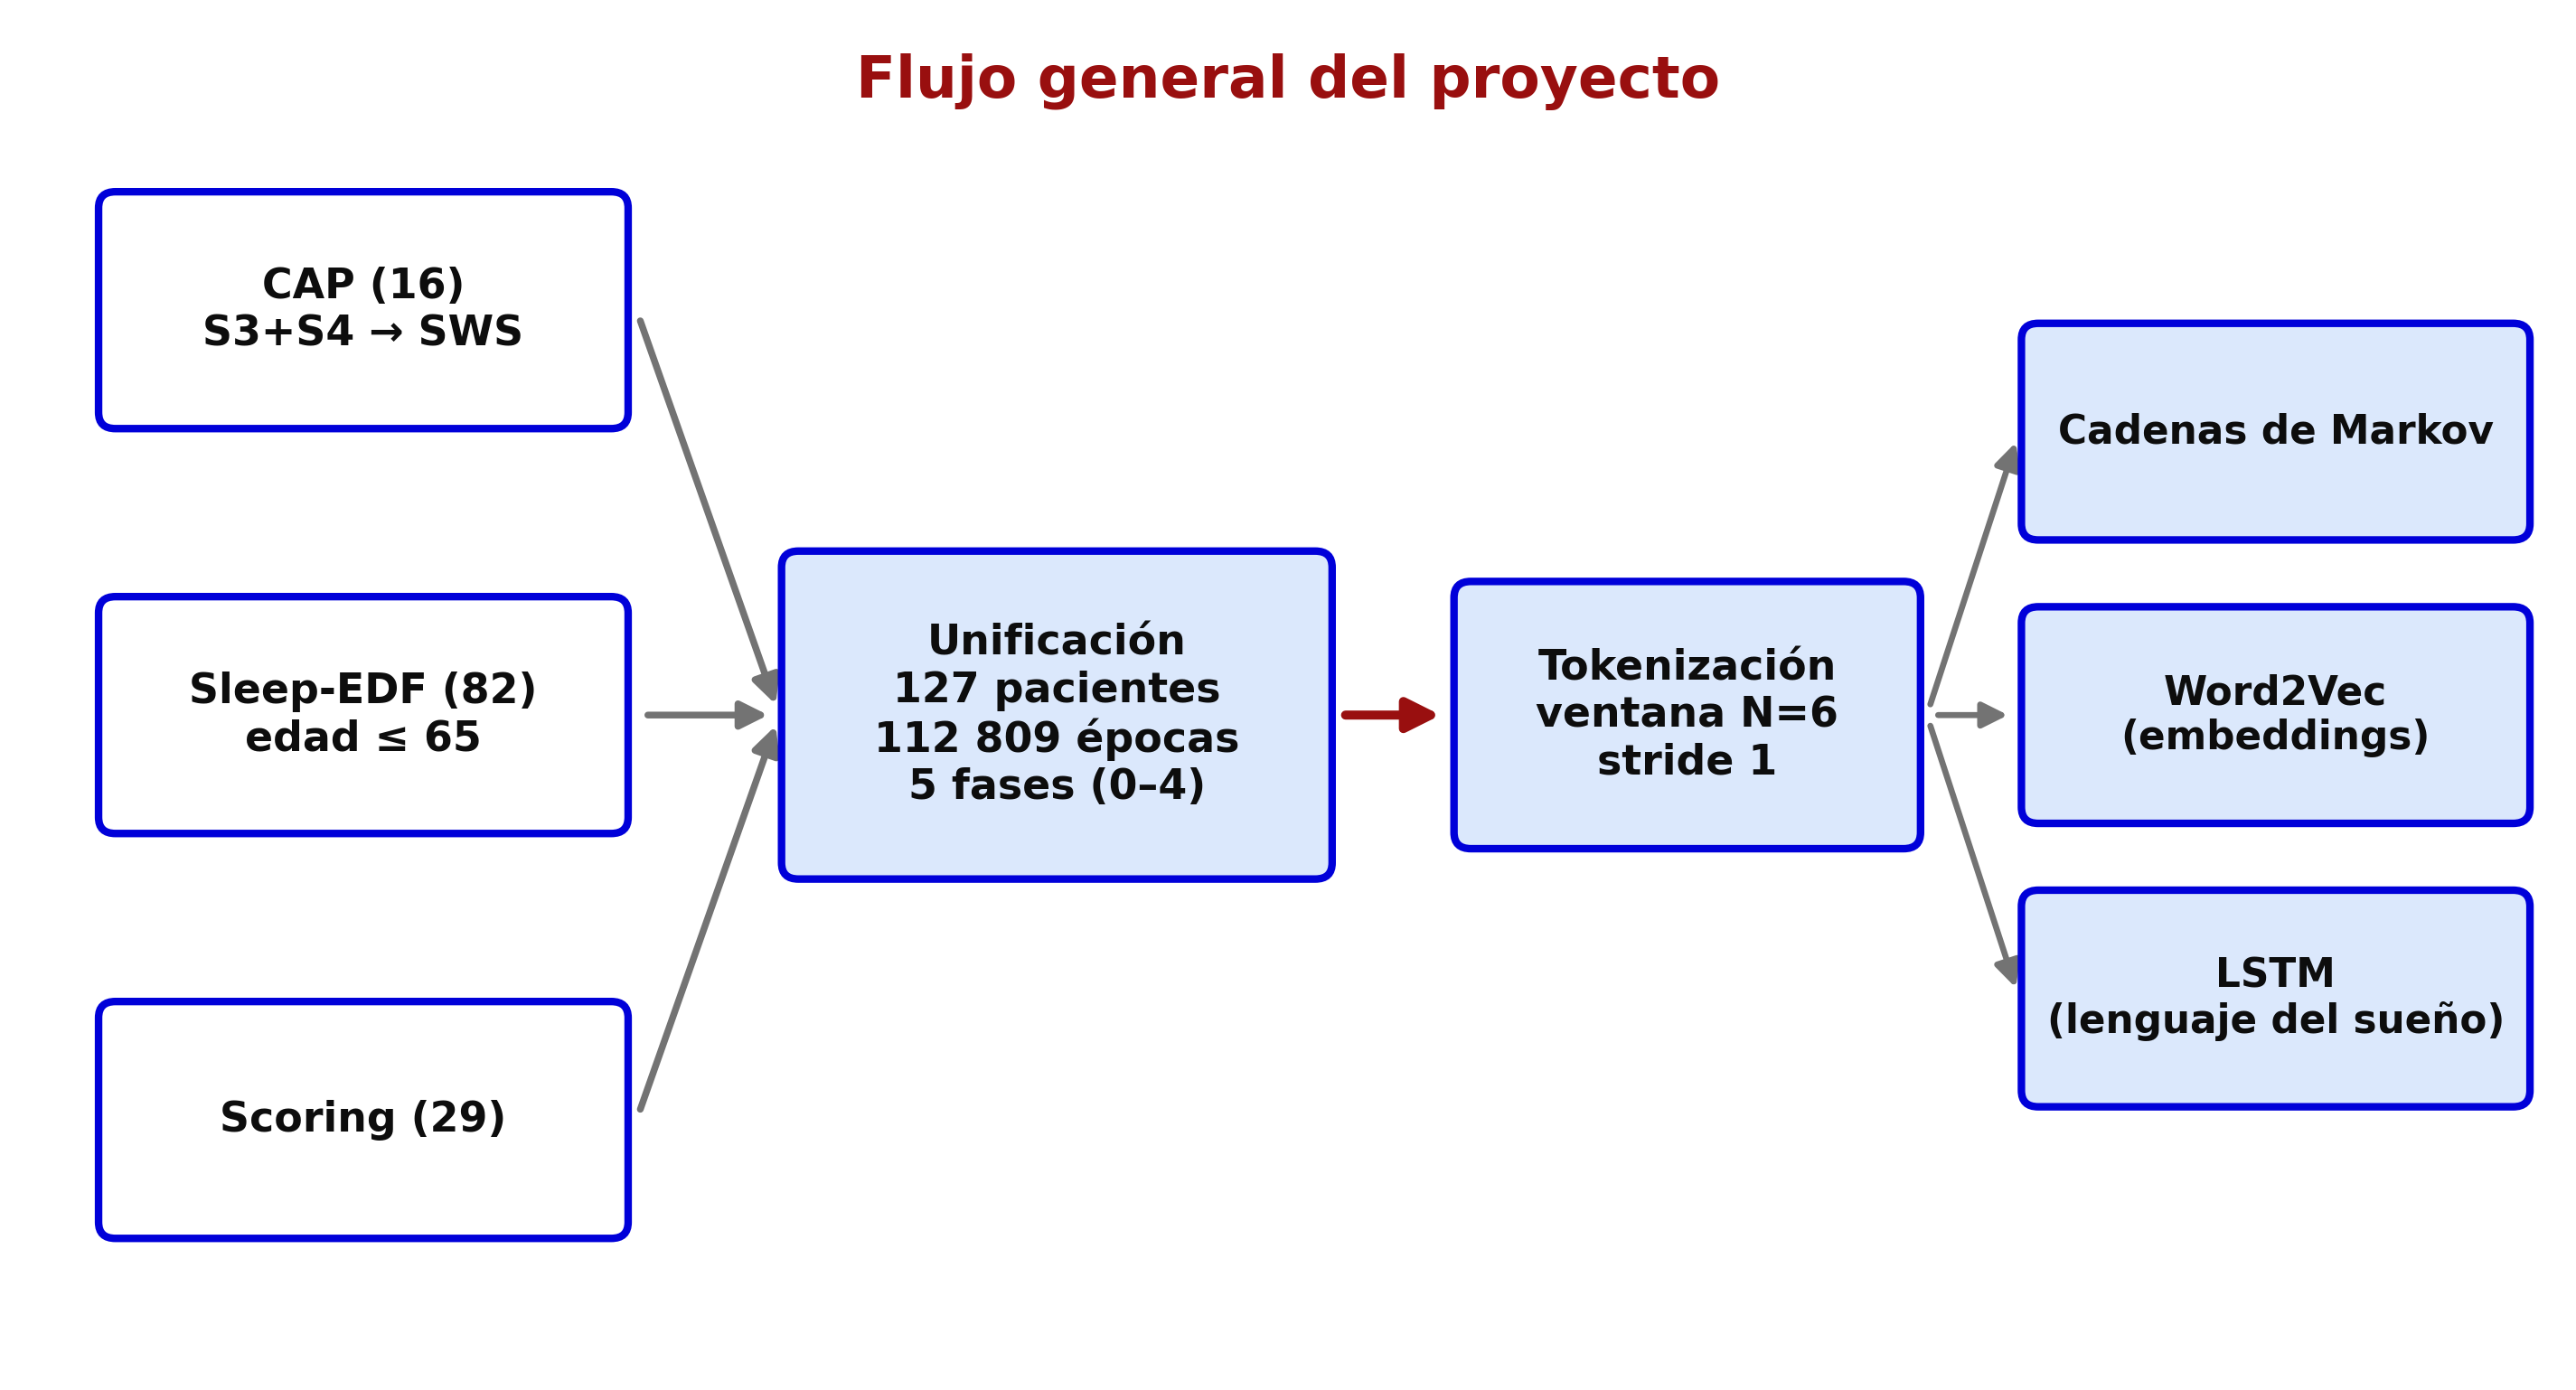
\includegraphics[width=\textwidth]{pipeline_general.png}
    \caption{Flujo general del proyecto: las tres fuentes de registros se unifican en una sola cohorte, se tokenizan mediante ventaneo deslizante y alimentan los modelos de análisis.}
    \label{fig:pipeline}
\end{figure}

\section{Descripción del Dataset}

Para construir un modelo robusto del sueño sano y, a la vez, disponer de potencia estadística suficiente, se unificaron tres fuentes independientes de registros polisomnográficos de personas sanas. La unificación se realiza de forma idempotente en el primer notebook del proyecto, que homogeneiza los identificadores, la codificación de fases y la demografía disponible.

\subsection{Población y Muestra}

La cohorte de sujetos sanos se compone de \textbf{127 pacientes}, provenientes de tres fuentes:

\begin{itemize}
    \item \textbf{CAP} (\textit{CAP Sleep Database}): 16 sujetos sanos.
    \item \textbf{Sleep-EDF} (\textit{Sleep Cassette}): 82 noches, restringidas a participantes de 65 años o menos.
    \item \textbf{SCO} (\textit{Scoring}): 29 registros del laboratorio interno.
\end{itemize}

En conjunto, la cohorte sana reúne \textbf{112\,809 épocas} de 30 segundos, equivalentes a \textbf{940.1 horas} de sueño. La Tabla \ref{tab:dataset_unificado} resume su composición. Los hipnogramas fueron estadificados manualmente por expertos siguiendo reglas estándar \citep{rechtschaffen1968manual}, con ventanas temporales (épocas) de \textbf{30 segundos}.

\begin{table}[htbp]
\centering
\caption{Composición del dataset unificado de sujetos sanos.}
\label{tab:dataset_unificado}
\begin{tabular}{lrrrr}
\hline
\textbf{Fuente} & \textbf{Pacientes} & \textbf{Épocas} & \textbf{Horas} & \textbf{Edad media} \\
\hline
CAP   & 16  & 15\,947  & 132.9 & 32.2 \\
EDF   & 82  & 70\,410  & 586.8 & 41.9 \\
SCO   & 29  & 26\,452  & 220.4 & --   \\
\hline
\textbf{Total} & \textbf{127} & \textbf{112\,809} & \textbf{940.1} & \textbf{40.3} \\
\hline
\end{tabular}
\end{table}

La distribución de fases, edades y duración por fuente se presenta en el Capítulo \ref{resultados}. La fuente SCO no dispone de metadatos demográficos, por lo que sus campos de sexo y edad quedan vacíos.

\subsection{Homogeneización entre Fuentes}

Cada fuente fue preprocesada para garantizar comparabilidad: en CAP se fusionaron las etapas S3 y S4 en sueño de ondas lentas (SWS) según el criterio de Rechtschaffen \& Kales; en Sleep-EDF se truncaron los tramos prolongados de vigilia previa y posterior al sueño y se filtró por edad ($\leq 65$ años); y en SCO se utilizó la estadificación limpia validada por expertos. Tras la unificación, los identificadores quedan prefijados por fuente (\texttt{CAP\_*}, \texttt{EDF\_*}, \texttt{SCO\_*}) y todas las fases comparten una única codificación.

\section{Preprocesamiento y Codificación}

\subsection{Sistema de Clasificación Unificado}

Cada fuente empleaba originalmente su propia codificación de estadios. Durante la unificación, todas las fases se mapearon a una codificación numérica común (0--5) mostrada en la Tabla \ref{tab:codificacion_original}.

\begin{table}[htbp]
\centering
\caption{Codificación unificada de estados de sueño en el dataset.}
\label{tab:codificacion_original}
\begin{tabular}{cl}
\hline
\textbf{Código} & \textbf{Estado} \\
\hline
0 & Vigilia (W) \\
1 & Sueño Ligero Etapa 1 (S1) \\
2 & Sueño Ligero Etapa 2 (S2) \\
3 & Sueño de Ondas Lentas (SWS = S3 + S4) \\
4 & Sueño REM \\
5 & Sin Clasificar (incluye Movimiento) \\
\hline
\end{tabular}
\end{table}

\subsection{Definición del Espacio de Estados}

La fusión de las etapas \textbf{S3 y S4} en una sola categoría de sueño de ondas lentas (SWS) se aplica en origen, dado que ambas representan sueño profundo delta y la distinción entre ellas es difusa en términos de dinámica de transición macroscópica. Las épocas \textbf{Sin Clasificar} (código 5, que agrupa movimiento y etiquetas ausentes) se tratan como ruido y se excluyen del cálculo de matrices de transición.

El ``vocabulario'' de fases del modelo queda constituido por \textbf{5 estados fundamentales}:
\begin{equation}
    \mathcal{S} = \{ \text{W}, \text{S1}, \text{S2}, \text{SWS}, \text{REM} \}
    \label{eq:vocabulario}
\end{equation}

La Tabla \ref{tab:codificacion_simplificada} resume el mapeo aplicado en cada fuente.

\begin{table}[htbp]
\centering
\caption{Mapeo de las etapas originales al espacio de estados unificado.}
\label{tab:codificacion_simplificada}
\small\setlength{\tabcolsep}{5pt}%
\begin{tabular}{cll}
\hline
\textbf{Código} & \textbf{Estado Unificado} & \textbf{Nota} \\
\hline
0 & Vigilia (W) & \\
1 & S1 & \\
2 & S2 & \\
3 & SWS & fusión de S3 y S4 \\
4 & REM & \\
5 & Sin Clasificar & movimiento y etiquetas ausentes (excluido) \\
\hline
\end{tabular}
\end{table}

\section{Determinación de la Escala Temporal}

Un problema central al aplicar modelos de n-gramas a series temporales fisiológicas es la elección del tamaño de ventana $N$. Una selección arbitraria puede cortar procesos biológicos de distinta escala o introducir artefactos estadísticos. En lugar de fijar $N$ a priori, se eligió de forma empírica sobre la cohorte unificada de 127 pacientes combinando tres criterios independientes.

\subsection{Criterios de Selección}

Para cada candidato de $N$ se construyen todos los n-gramas del corpus y se evalúan:

\begin{enumerate}
    \item \textbf{Ley de Zipf ($\beta$):} se ordenan los n-gramas por frecuencia descendente y se ajusta por mínimos cuadrados la recta $\log_{10}(\text{frecuencia}) = a - \beta \log_{10}(\text{rango})$. Una distribución de tipo lenguaje natural tiene $\beta \approx 1$.
    \item \textbf{Calidad del ajuste ($R^2$):} mide cuán limpia es la ley de potencia. Un $R^2$ alto indica una recta log-log bien definida y no ruido.
    \item \textbf{Cobertura de los bloques de S2:} la fase 2 aparece en bloques de épocas consecutivas. Se mide qué fracción de esos bloques tiene longitud mayor o igual a $N$; así, una ventana que cabe dentro del bloque típico captura una unidad fisiológica completa.
\end{enumerate}

\subsection{Barrido y Criterio Combinado}

Se realizó un barrido amplio de $N$ (de 1 hasta 100) para caracterizar el comportamiento global, y un ranking fino sobre los candidatos $N \in \{5,6,7,8,9,10,12,15\}$. El detalle numérico se presenta en el Capítulo \ref{resultados}; aquí se resume la decisión.

El valor de $\beta$ crece hasta $N=2$ y luego decrece monótonamente, cruzando $\beta = 1$ entre $N=8$ y $N=10$. Si se atendiera únicamente a $|\beta - 1|$, el ganador sería $N=10$. Sin embargo, ese criterio aislado ignora la calidad del ajuste y la coherencia fisiológica. Al combinar los tres criterios en un ranking por posición media, el mejor balance lo obtiene:

\begin{equation}
    N = 6 \text{ épocas} \quad (\approx 3 \text{ minutos})
    \label{eq:ventana}
\end{equation}

En $N=6$ el ajuste log-log alcanza su mayor calidad ($R^2 = 0.977$) y la ventana sigue cabiendo dentro de casi la mitad de los bloques de S2 (cobertura del 47.3\%), mientras que $\beta = 1.60$ se mantiene en un rango compatible con estructura de lenguaje. Es decir, $N=6$ no minimiza la distancia a Zipf, pero es el tamaño que mejor concilia los tres criterios simultáneamente. Este valor define el token para el resto del análisis vectorial.

\section{Entrenamiento de Embeddings (Word2Vec)}

\subsection{Tokenización Temporal (N-gramas)}

A diferencia del análisis estadístico tradicional que trata cada época como un punto independiente, este estudio define la unidad mínima de análisis (token) como una \textbf{secuencia temporal de 6 épocas consecutivas}.

Cada token se codifica como una cadena del tipo \texttt{a-b-c-d-e-f}, donde cada letra representa el estado simplificado de una época. Por ejemplo, el token \texttt{2-2-2-2-2-3} representa una ventana donde predomina S2 y la última época corresponde a SWS.

\subsection{Generación del Corpus y Selección del Stride}

El corpus de entrenamiento se generó mediante un \textbf{ventaneo deslizante (sliding window)} con los siguientes parámetros:
\begin{itemize}
    \item \textbf{Tamaño de ventana:} $N = 6$ épocas
    \item \textbf{Paso (stride):} 1 época (máximo solapamiento)
\end{itemize}

\begin{figure}[htbp]
    \centering
    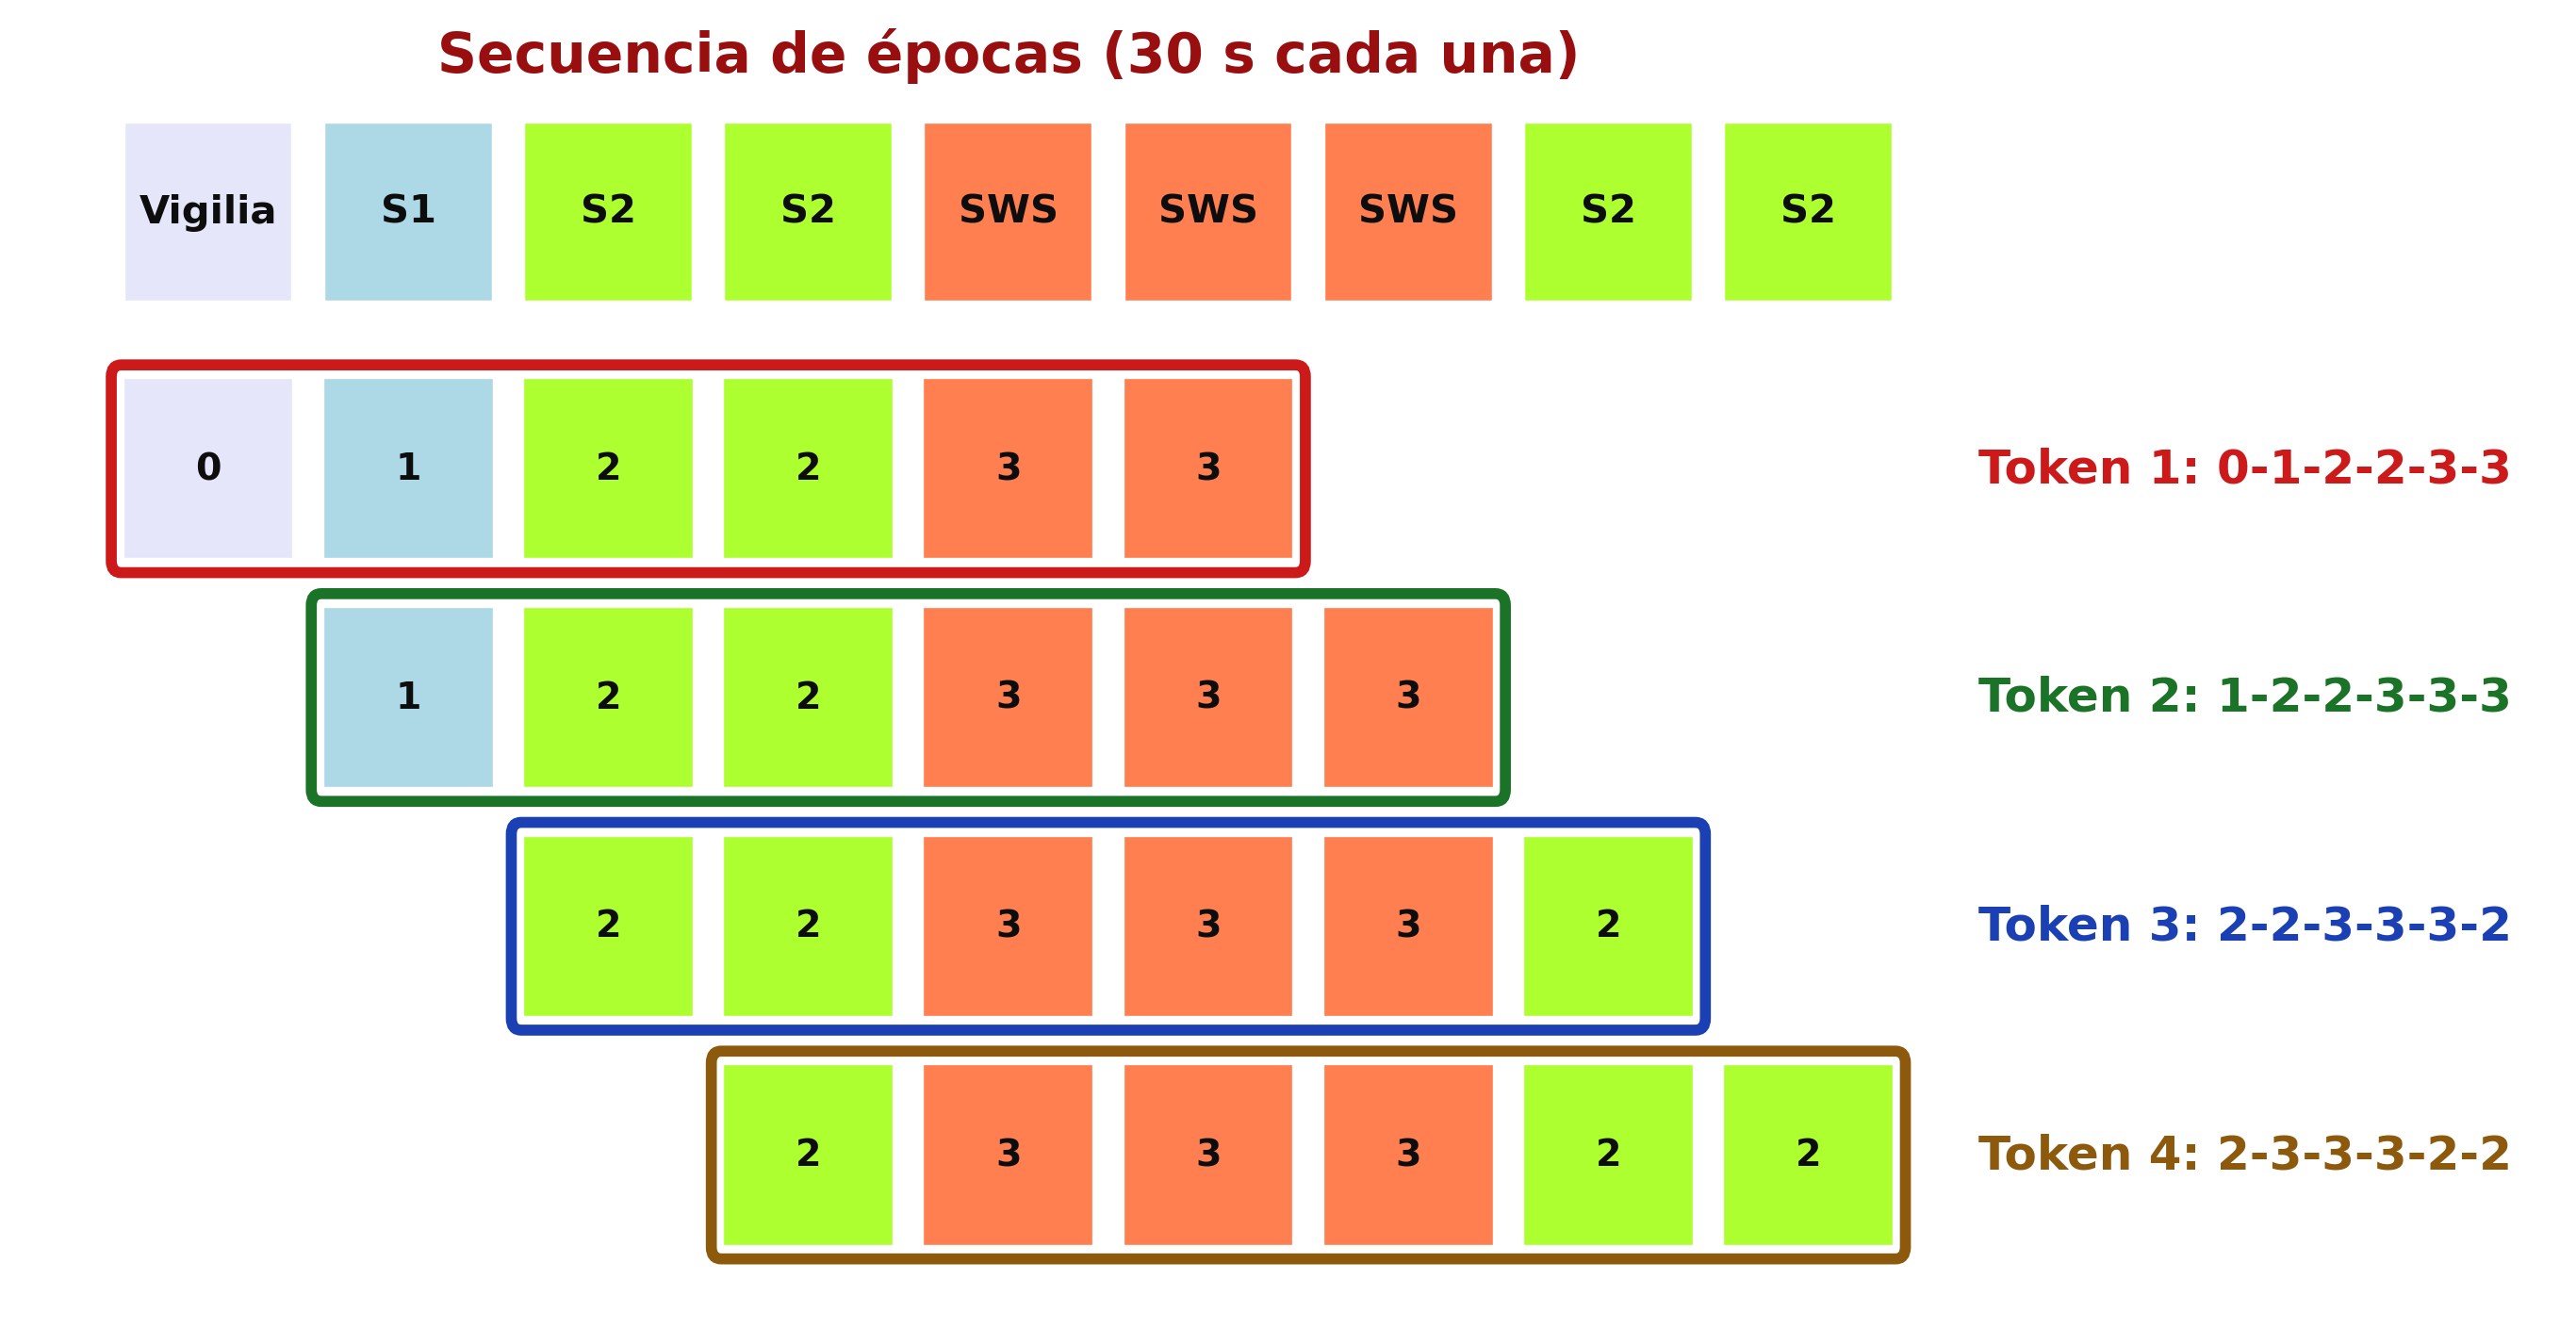
\includegraphics[width=\textwidth]{ventana_deslizante.png}
    \caption{Ventaneo deslizante con $N=6$ y paso de una época. Cada token agrupa seis épocas consecutivas y la ventana avanza de una en una, de modo que tokens contiguos comparten cinco de sus seis épocas.}
    \label{fig:ventana_deslizante}
\end{figure}

\textbf{Justificación del Stride:} Se adoptó un paso de una sola época (solapamiento máximo) en lugar de un ventaneo sin solapamiento. La razón es doble. Primero, la \textbf{robustez estadística}: con paso 1 cada noche aporta tantas ventanas como épocas tiene, lo que multiplica el volumen del corpus y permite estimar representaciones estables incluso para 6-gramas poco frecuentes; un paso igual a $N$ reduciría el corpus en un factor de seis y dejaría sin soporte a buena parte del vocabulario. Segundo, la \textbf{coherencia fisiológica}: el sueño es un proceso progresivo y continuo, de modo que ventanas que comparten cinco de sus seis épocas describen estados vecinos en una trayectoria suave; preservar ese solapamiento mantiene la continuidad de las transiciones, mientras que un ventaneo disjunto fragmentaría la secuencia y borraría los cambios graduales entre fases. El costo conocido de esta decisión es la autocorrelación entre ventanas consecutivas: como tokens contiguos comparten cinco de sus seis épocas, las $\sim$110\,000 ventanas \textbf{no son observaciones independientes}, por lo que el \textit{tamaño efectivo de muestra} es sustancialmente menor que el conteo bruto y los intervalos de confianza ingenuos subestimarían la incertidumbre. Asumimos este sesgo como contrapartida del mayor tamaño y suavidad del corpus; para verificar que las conclusiones no son un artefacto del solapamiento, el análisis clave se repite con un paso disjunto ($\text{stride}=N$) ---que elimina la autocorrelación entre ventanas a costa de un corpus seis veces menor---, cuyo resultado se reporta en la Sección \ref{sec:deslizador_stride}.

El corpus unificado contiene del orden de \textbf{110\,000 ventanas} de 6 épocas. Tras filtrar los hápax (tokens con frecuencia menor a 2), el vocabulario de 6-gramas quedó en \textbf{1\,503 tokens}. El token dominante es \texttt{2-2-2-2-2-2} (S2 sostenido), coherente con que S2 ocupa cerca de la mitad del tiempo nocturno.

\subsection{Arquitectura del Modelo}

Se implementó el modelo \textbf{Word2Vec Skip-Gram} \citep{mikolov2013efficient} en PyTorch (optimizador Adam, $\text{lr}=0.01$, función de pérdida de entropía cruzada). A lo largo del trabajo se entrenaron \textbf{tres variantes} del modelo según el análisis: una sobre \textbf{unigramas} (para la validación topológica de las fases individuales) y dos sobre \textbf{6-gramas} que se diferencian únicamente en el umbral de frecuencia mínima (\texttt{min\_freq}). La Tabla \ref{tab:hiperparametros_w2v} las documenta de forma explícita para garantizar la trazabilidad.

\begin{table}[htbp]
\centering
\caption{Hiperparámetros de las tres variantes de Word2Vec entrenadas. Comparten optimizador (Adam, lr~0.01), tamaño de batch (512) y semilla (42).}
\label{tab:hiperparametros_w2v}
\footnotesize\setlength{\tabcolsep}{4pt}%
\begin{tabular}{lccc}
\hline
\textbf{Parámetro} & \textbf{Unigramas} & \textbf{6-gramas} & \textbf{6-gramas (mf1)} \\
\hline
Dimensión del embedding & 24 & 32 & 32 \\
Ventana contextual & 3 & 1 & 1 \\
Épocas de entrenamiento & 20 & 30 & 30 \\
Frecuencia mínima (\texttt{min\_freq}) & 2 & 2 & 1 \\
Tamaño del vocabulario & 6 & 1\,503 & 2\,817 \\
Uso principal & Topología 1g & Topología 6g & Deslizador y LSTM \\
\hline
\end{tabular}
\end{table}

La ventana contextual de 1 en los modelos de 6-gramas se justifica porque cada token ya encapsula 6 épocas de contexto temporal; contextos más amplios serían redundantes (en unigramas, donde el token es una sola época, se usa ventana 3).

\textbf{Nota sobre la variante \texttt{mf1}.} Los dos experimentos centrales basados en 6-gramas ---el \emph{Deslizador} (Sección \ref{sec:deslizador_metodo}) y el modelo recurrente LSTM--- utilizan una variante entrenada con \texttt{min\_freq}=1 (vocabulario de 2\,817 tokens), en lugar del modelo de topología con \texttt{min\_freq}=2 (1\,503 tokens). La razón es que estos análisis recorren secuencias de transición que incluyen 6-gramas poco frecuentes (cercanos a hápax); descartarlos dejaría sin representación a varias ventanas de la trayectoria. El modelo subrogado correspondiente se entrena con el mismo criterio \texttt{min\_freq}=1 sobre la secuencia permutada.

\section{Análisis de Trayectorias: Interpolación de Estados}
\label{sec:deslizador_metodo}

El experimento del \textbf{Deslizador} consiste en observar cómo evoluciona la representación vectorial de una ventana de S2 conforme se infiltran progresivamente épocas de un estado destino (REM o SWS). Procede sobre secuencias sintéticas e ilustra la organización geométrica del espacio de embeddings; la evidencia de anticipación sobre datos reales se aborda después con el modelo recurrente.

\subsection{Diseño del Experimento}

Se construyeron secuencias sintéticas que representan la transición progresiva desde un estado ``puro'' de S2 hacia los estados destino. La Figura \ref{fig:interpolacion} ilustra este proceso de interpolación gradual.

\begin{figure}[htbp]
    \centering
    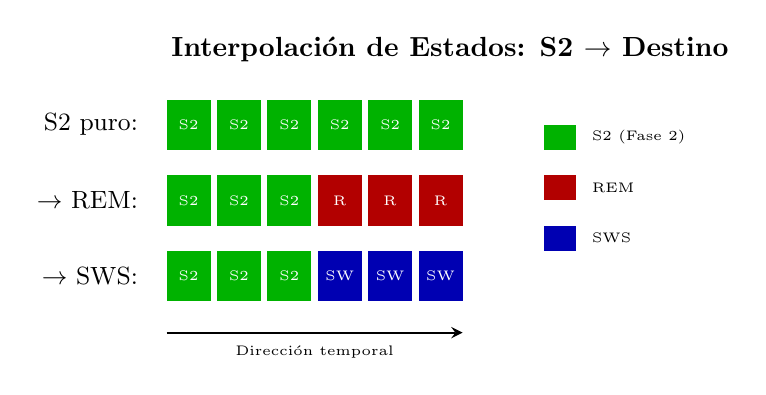
\begin{tikzpicture}[scale=0.8]
        % Título
        \node[font=\bfseries] at (4.5, 3.2) {Interpolación de Estados: S2 $\rightarrow$ Destino};
        
        % Estado inicial S2 puro
        \node[font=\small, anchor=east] at (-0.3, 2) {S2 puro:};
        \foreach \x in {0,...,5} {
            \fill[green!70!black] (\x*0.8, 1.6) rectangle (\x*0.8+0.7, 2.4);
            \node[font=\tiny, white] at (\x*0.8+0.35, 2) {S2};
        }
        
        % Transición hacia REM (rojo)
        \node[font=\small, anchor=east] at (-0.3, 0.8) {$\rightarrow$ REM:};
        \fill[green!70!black] (0, 0.4) rectangle (0.7, 1.2);
        \fill[green!70!black] (0.8, 0.4) rectangle (1.5, 1.2);
        \fill[green!70!black] (1.6, 0.4) rectangle (2.3, 1.2);
        \fill[red!70!black] (2.4, 0.4) rectangle (3.1, 1.2);
        \fill[red!70!black] (3.2, 0.4) rectangle (3.9, 1.2);
        \fill[red!70!black] (4.0, 0.4) rectangle (4.7, 1.2);
        \node[font=\tiny, white] at (0.35, 0.8) {S2};
        \node[font=\tiny, white] at (1.15, 0.8) {S2};
        \node[font=\tiny, white] at (1.95, 0.8) {S2};
        \node[font=\tiny, white] at (2.75, 0.8) {R};
        \node[font=\tiny, white] at (3.55, 0.8) {R};
        \node[font=\tiny, white] at (4.35, 0.8) {R};
        
        % Transición hacia SWS (azul)
        \node[font=\small, anchor=east] at (-0.3, -0.4) {$\rightarrow$ SWS:};
        \fill[green!70!black] (0, -0.8) rectangle (0.7, 0);
        \fill[green!70!black] (0.8, -0.8) rectangle (1.5, 0);
        \fill[green!70!black] (1.6, -0.8) rectangle (2.3, 0);
        \fill[blue!70!black] (2.4, -0.8) rectangle (3.1, 0);
        \fill[blue!70!black] (3.2, -0.8) rectangle (3.9, 0);
        \fill[blue!70!black] (4.0, -0.8) rectangle (4.7, 0);
        \node[font=\tiny, white] at (0.35, -0.4) {S2};
        \node[font=\tiny, white] at (1.15, -0.4) {S2};
        \node[font=\tiny, white] at (1.95, -0.4) {S2};
        \node[font=\tiny, white] at (2.75, -0.4) {SW};
        \node[font=\tiny, white] at (3.55, -0.4) {SW};
        \node[font=\tiny, white] at (4.35, -0.4) {SW};
        
        % Leyenda
        \fill[green!70!black] (6, 1.6) rectangle (6.5, 2);
        \node[font=\tiny, anchor=west] at (6.6, 1.8) {S2 (Fase 2)};
        \fill[red!70!black] (6, 0.8) rectangle (6.5, 1.2);
        \node[font=\tiny, anchor=west] at (6.6, 1) {REM};
        \fill[blue!70!black] (6, 0) rectangle (6.5, 0.4);
        \node[font=\tiny, anchor=west] at (6.6, 0.2) {SWS};
        
        % Flecha de tiempo
        \draw[-stealth, thick] (0, -1.3) -- (4.7, -1.3);
        \node[font=\tiny] at (2.35, -1.6) {Dirección temporal};
    \end{tikzpicture}
    \caption{Diagrama del experimento de Interpolación de Estados. Se construyen secuencias sintéticas que transitan gradualmente desde S2 puro hacia REM (rojo) o SWS (azul), permitiendo medir cómo evoluciona el vector en el espacio latente.}
    \label{fig:interpolacion}
\end{figure}

Formalmente, las secuencias de interpolación se definen como:
\begin{itemize}
    \item \textbf{Estado inicial (S2 puro):} \texttt{2-2-2-2-2-2}
    \item \textbf{Transición hacia REM:} \texttt{2-2-2-2-2-4} $\rightarrow$ \texttt{2-2-2-2-4-4} $\rightarrow$ ... $\rightarrow$ \texttt{4-4-4-4-4-4}
    \item \textbf{Transición hacia SWS:} \texttt{2-2-2-2-2-3} $\rightarrow$ \texttt{2-2-2-2-3-3} $\rightarrow$ ... $\rightarrow$ \texttt{3-3-3-3-3-3}
\end{itemize}

\subsection{Métrica: Distancia Coseno}

Para cada paso de la transición, se calculó la \textbf{Distancia Coseno} entre el vector del estado puro (S2) y el vector de la secuencia en transición:

\begin{equation}
    d_{\cos}(\vec{v}_1, \vec{v}_2) = 1 - \frac{\vec{v}_1 \cdot \vec{v}_2}{\|\vec{v}_1\| \|\vec{v}_2\|}
    \label{eq:distancia_coseno}
\end{equation}

Valores cercanos a 0 indican alta similitud (vectores paralelos); valores cercanos a 2 indican máxima disimilitud (vectores opuestos).

\subsection{Hipótesis de Bifurcación}

Si la Fase 2 posee ``memoria latente'' sobre su destino, las trayectorias hacia REM y SWS deberían \textbf{divergir antes} de que el símbolo destino sea mayoritario en el n-grama. Es decir, el modelo debería detectar la ``intención'' del cerebro antes de que ocurra el cambio clínico visible.

\section{Análisis de Estabilidad: Matrices de Transición de Markov}

Complementando el análisis vectorial, se implementó un enfoque matricial para cuantificar la \textbf{resistencia al cambio} de cada fase.

\subsection{Construcción de Matrices}

Se calcularon \textbf{Matrices de Transición de Markov} de tamaño $5 \times 5$ (una por cada estado del vocabulario simplificado), donde cada elemento $P_{ij}$ representa:

\begin{equation}
    P_{ij} = P(\text{Estado}_{t+1} = j \mid \text{Estado}_t = i)
    \label{eq:prob_transicion}
\end{equation}

\subsection{Análisis Con y Sin Diagonal}

Se generaron dos versiones de las matrices:
\begin{itemize}
    \item \textbf{Con Diagonal:} Incluye la probabilidad de permanencia $P(i|i)$. Revela la \textbf{inercia} o estabilidad de cada fase.
    \item \textbf{Sin Diagonal:} Normaliza las probabilidades excluyendo la auto-transición. Revela \textbf{hacia dónde huye} el cerebro cuando abandona una fase.
\end{itemize}

\subsection{Análisis por Ciclos}

Reconociendo la no-estacionariedad del sueño, las matrices se calcularon de forma independiente para cada \textbf{ciclo ultradiano} (aproximadamente 90 minutos):
\begin{itemize}
    \item Ciclo 1 (0-90 min): Presión homeostática máxima
    \item Ciclo 2 (90-180 min): Transición
    \item Ciclo 3+ (180+ min): Predominancia circadiana
\end{itemize}

Este análisis permite observar cómo evoluciona la \textbf{estabilidad del sueño} a lo largo de la noche.

\section{Validación: Datos Subrogados (Surrogates)}

Para descartar que los patrones observados sean artefactos estadísticos de la frecuencia de los símbolos, se implementó un procedimiento de \textbf{validación con datos subrogados (shuffling temporal)}.

\subsection{Procedimiento}

\begin{enumerate}
    \item Se aleatorizó el orden temporal de las épocas dentro de cada hipnograma, destruyendo la estructura secuencial pero preservando la distribución de frecuencias.
    \item Se repitió el entrenamiento del modelo Word2Vec con los datos revueltos.
    \item Se recalcularon las trayectorias del experimento del ``Deslizador''.
\end{enumerate}

\subsection{Criterio de Éxito}

Si la divergencia entre las trayectorias REM y SWS \textbf{desaparece} en los datos subrogados, entonces la estructura observada en los datos reales es una propiedad \textbf{biológica genuina} y no un artefacto de la distribución estadística.

\section{Modelo de Lenguaje Recurrente (LSTM)}

El experimento del Deslizador examina vectores aislados. Para evaluar si la información secuencial permite \textit{predecir} la dinámica nocturna, se entrenó una red recurrente \textbf{LSTM} como modelo de lenguaje del sueño.

\subsection{Tarea y Arquitectura}

A diferencia de un clasificador que observa un único 6-grama, el LSTM se despliega sobre la \textbf{noche completa}: recibe la secuencia de 6-gramas de toda la noche (cada token codificado con el embedding Word2Vec \textbf{congelado}) y en cada paso predice la \textbf{siguiente época} (W, S1, S2, SWS, REM). Es la tarea de ``predecir la siguiente palabra'' del procesamiento de lenguaje natural, pero con memoria temporal de largo alcance: el estado oculto acumula el historial completo hasta el instante actual. El embedding se mantiene fijo para que la comparación con los modelos basales sea atribuible a la dinámica recurrente y no a un reentrenamiento de las representaciones. La Figura \ref{fig:lstm} ilustra este despliegue paso a paso.

\begin{figure}[htbp]
    \centering
    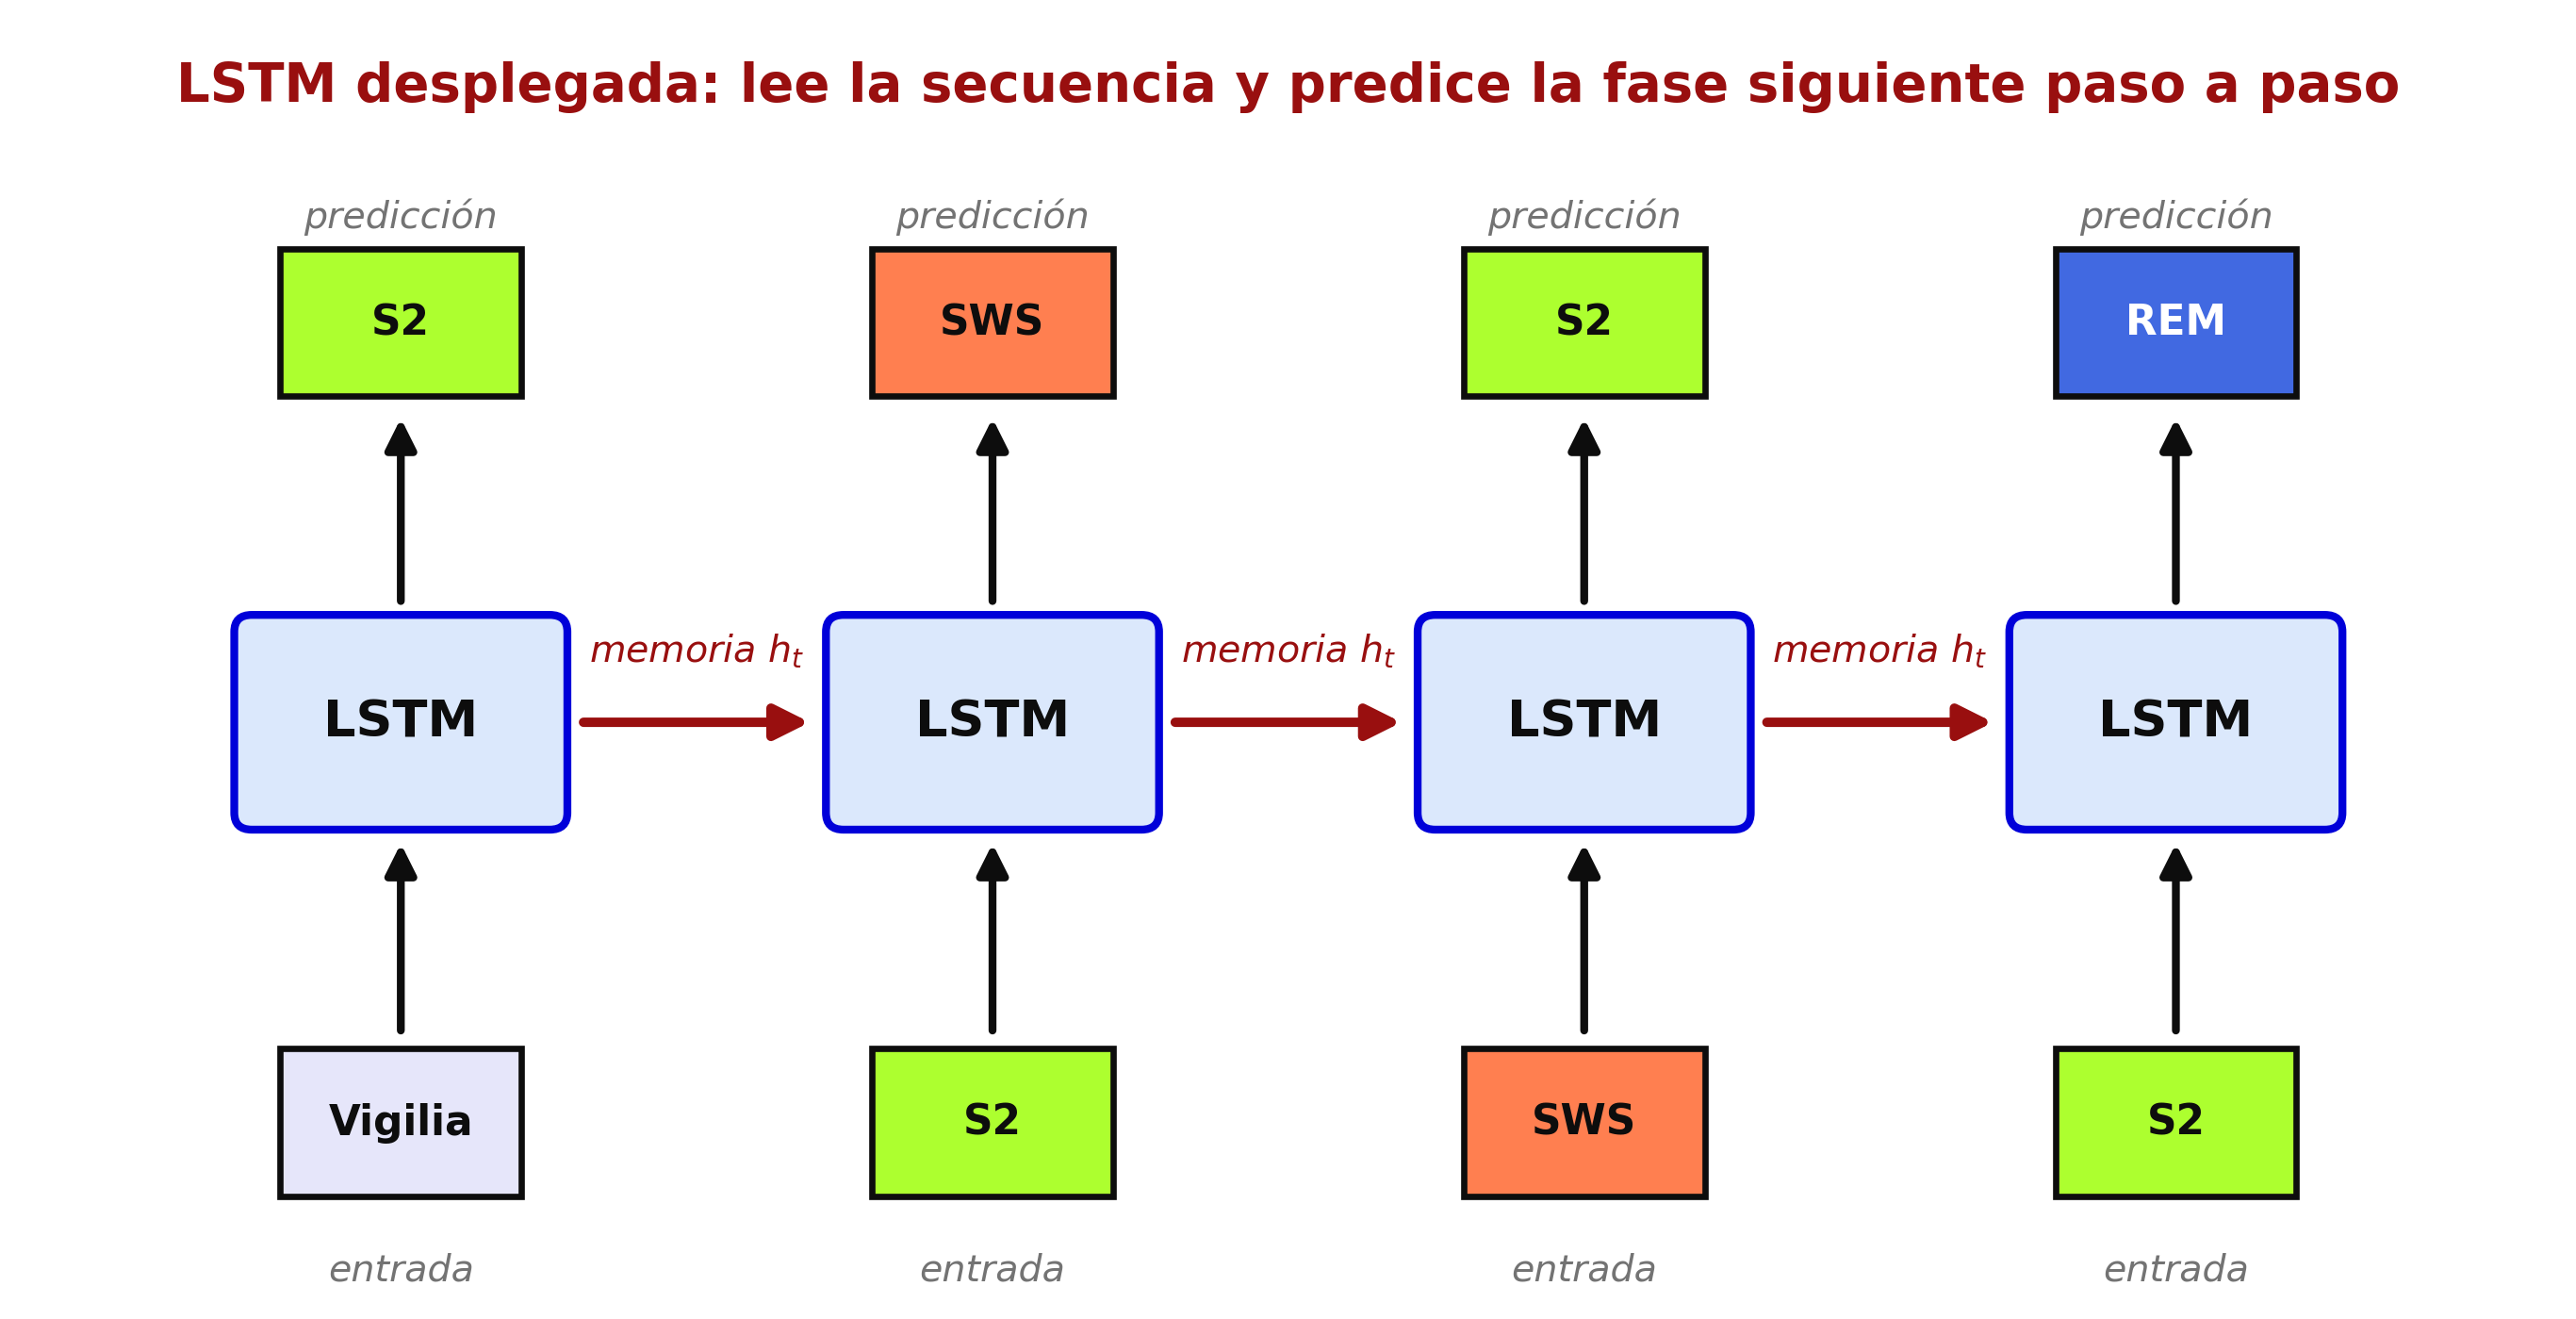
\includegraphics[width=\textwidth]{lstm_desplegada.png}
    \caption{Red LSTM desplegada sobre la secuencia de la noche. En cada paso recibe el embedding del 6-grama actual y predice la fase siguiente, propagando el estado de memoria $h_t$ que acumula el historial temporal.}
    \label{fig:lstm}
\end{figure}

Concretamente, la red consta de tres componentes (Tabla \ref{tab:hiperparametros_lstm}): (i)~una capa de \textit{embedding} que asigna a cada índice de 6-grama su vector Word2Vec de 32 dimensiones y que permanece \textbf{congelada} durante todo el entrenamiento; (ii)~una única capa \textbf{LSTM} de 128 unidades ocultas, desplegada sobre la noche completa, que propaga el estado de memoria $h_t$ acumulando el historial hasta el instante actual; y (iii)~una capa lineal que proyecta el estado oculto de cada paso a las cinco fases del sueño. En total se entrenan unos 83\,600 parámetros. El modelo se optimiza con \textbf{entropía cruzada ponderada por la frecuencia inversa de cada clase} ---para contrarrestar el marcado desbalance del sueño, donde la Fase 2 domina y S1 es escasa--- mediante Adam ($\text{lr}=10^{-3}$) sobre lotes de 16 noches, durante un máximo de 40 épocas con \textbf{parada temprana} (paciencia de 6 épocas sobre la exactitud de validación).

\begin{table}[htbp]
\centering
\caption{Arquitectura e hiperparámetros de entrenamiento de la red LSTM.}
\label{tab:hiperparametros_lstm}
\footnotesize\setlength{\tabcolsep}{4pt}%
\begin{tabular}{ll}
\hline
\textbf{Componente / Hiperparámetro} & \textbf{Valor} \\
\hline
Embedding de entrada & Word2Vec 6-gramas (\texttt{mf1}), 32 dim, \textbf{congelado} \\
Capa recurrente & LSTM, 1 capa, 128 unidades ocultas \\
Capa de salida & Lineal, $128 \rightarrow 5$ (una \textit{logit} por fase) \\
Parámetros entrenables & $\approx$83\,600 \\
Función de pérdida & Entropía cruzada ponderada por clase \\
Optimizador & Adam, $\text{lr}=10^{-3}$ \\
Tamaño de lote & 16 noches \\
Épocas (máx.) / parada temprana & 40 / paciencia 6 \\
Semilla & 42 \\
\hline
\end{tabular}
\end{table}

\subsection{Construcción de Secuencias y Partición Sujeto-Disjunta}

Cada noche se transforma en una secuencia de pasos de predicción: en la posición $t$, la entrada es el 6-grama que abarca las épocas $[t-6,\,t-1]$ ---representado por su índice en el vocabulario Word2Vec--- y el objetivo es la fase observada en la época $t$, es decir, la \textbf{siguiente} época. Las escasas posiciones cuyo 6-grama queda fuera de vocabulario (0.09\,\% del total) se descartan.

La partición en entrenamiento y prueba se realiza \textbf{por sujeto}: los 127 pacientes se reparten de forma \textbf{disjunta} en un 80\,\% para entrenamiento (101 sujetos) y un 20\,\% para prueba (26 sujetos), de modo que todas las noches ---y por tanto todas las ventanas--- de un mismo paciente quedan íntegramente en un único conjunto. Esta decisión es deliberada y crítica: puesto que el corpus se genera con solapamiento máximo, en el que ventanas contiguas comparten cinco de sus seis épocas (Figura \ref{fig:ventana_deslizante}), una partición aleatoria por época o por ventana provocaría \textbf{fuga de datos} ---ventanas casi idénticas del mismo sujeto caerían a la vez en entrenamiento y prueba, inflando las métricas precisamente por la autocorrelación inherente al solapamiento---. Al separar por paciente, esa fuga queda excluida por construcción: el modelo se evalúa exclusivamente sobre sujetos que no observó durante el entrenamiento, por lo que las métricas reportadas ---incluida la matriz de confusión--- reflejan la \textbf{generalización a nuevos individuos} y no la memorización de ventanas solapadas.

\subsection{Modelos Basales y Controles}

El desempeño del LSTM se contrasta con dos basales triviales y un control:

\begin{itemize}
    \item \textbf{Persistencia:} predice que la fase siguiente es igual a la actual.
    \item \textbf{Markov de orden 1:} predice la fase más probable dada únicamente la fase actual.
    \item \textbf{Control \textit{shuffled}:} el mismo LSTM entrenado sobre secuencias permutadas dentro de cada paciente, para comprobar si captura orden temporal o solo frecuencias marginales.
\end{itemize}

\subsection{Evaluación Honesta en Transiciones}

Dado que el sueño es altamente persistente (una fase suele repetirse muchas épocas seguidas), la exactitud global premia a quien simplemente ``no cambia''. Por ello se reporta además una métrica restringida a las \textbf{épocas de transición} (aquellas donde la fase efectivamente cambia), que es donde un modelo aporta valor real. Finalmente se analiza la \textbf{bifurcación de S2}: alineando todas las corridas que parten de S2 en el instante $t=0$ y midiendo la probabilidad asignada a SWS y a REM en los pasos previos, se evalúa si el modelo anticipa el destino antes de la transición.

\section{Herramientas y Reproducibilidad}

El análisis se implementó en Python 3.10 utilizando las siguientes bibliotecas:
\begin{itemize}
    \item \textbf{NumPy} y \textbf{Pandas}: Manipulación y procesamiento de datos
    \item \textbf{PyTorch}: Implementación del modelo Word2Vec (Skip-Gram)
    \item \textbf{SciPy}: Cálculo de distancias (similitud coseno)
    \item \textbf{Plotly}: Visualización interactiva 2D y 3D
    \item \textbf{UMAP} \citep{mcinnes2018umap}: Reducción de dimensionalidad para visualización
\end{itemize}

\subsection{Configuración de UMAP para Visualización}

Dado que UMAP es un algoritmo sensible a sus hiperparámetros, documentamos la configuración exacta utilizada para garantizar la reproducibilidad de las visualizaciones:

\begin{table}[htbp]
\centering
\caption{Hiperparámetros de UMAP para la proyección de embeddings.}
\label{tab:hiperparametros_umap}
\begin{tabular}{ll}
\hline
\textbf{Parámetro} & \textbf{Valor} \\
\hline
\texttt{n\_neighbors} & 15 \\
\texttt{min\_dist} & 0.1 \\
\texttt{metric} & cosine \\
\texttt{n\_components} & 2 (para gráficas 2D) \\
\texttt{random\_state} & 42 \\
\hline
\end{tabular}
\end{table}

\textbf{Nota sobre \texttt{n\_neighbors}:} Este parámetro controla el balance entre estructura local y global. Un valor de 15 preserva vecindades cercanas sin perder la topología global del espacio de embeddings. Valores menores (ej. 5) enfatizarían clústeres más compactos pero podrían fragmentar las trayectorias continuas; valores mayores (ej. 50) suavizarían excesivamente la estructura.

El código fuente y los notebooks de análisis están disponibles en el repositorio del proyecto para garantizar la reproducibilidad de los resultados.

\chapter{Resultados}
\chaptermark{Resultados}
\label{resultados}

En este capítulo se presentan los hallazgos cuantitativos derivados del modelado híbrido de la arquitectura del sueño. Los resultados se organizan siguiendo la lógica de descubrimiento: primero el análisis estocástico basal (validación de la estructura del sueño mediante Cadenas de Markov), luego la búsqueda de la escala temporal óptima (donde convergen la estadística y la fisiología), seguido de la dinámica de transiciones vectoriales y su validación con datos subrogados, y finalmente el modelado predictivo mediante una red recurrente LSTM, que pone a prueba la anticipación de las transiciones sobre datos reales.

\section{Análisis Estocástico Basal: Cadenas de Markov}

Antes de aplicar modelos complejos de representación vectorial, es necesario validar que los datos poseen la estructura markoviana esperada para un sueño fisiológico sano. Este análisis cumple dos objetivos: (1) confirmar la calidad del dataset y (2) establecer una línea base cuantitativa contra la cual medir los aportes de los modelos posteriores.

\subsection{Matriz de Transición Global}

Se calculó la \textbf{Matriz de Transición de Markov} a partir de todos los bigramas (pares de épocas consecutivas) extraídos de los 127 sujetos del dataset unificado (112 809 épocas). El análisis se restringe a las cinco fases fisiológicas (las épocas sin clasificar se excluyen). La Figura \ref{fig:matriz_global} presenta el resultado en sus dos normalizaciones: la global (cada celda es la fracción del total de transiciones) y la de por renglón (cada celda es $P(j|i)$, la probabilidad de ir a la fase $j$ dado que se está en $i$).

\begin{figure}[htbp]
    \centering
    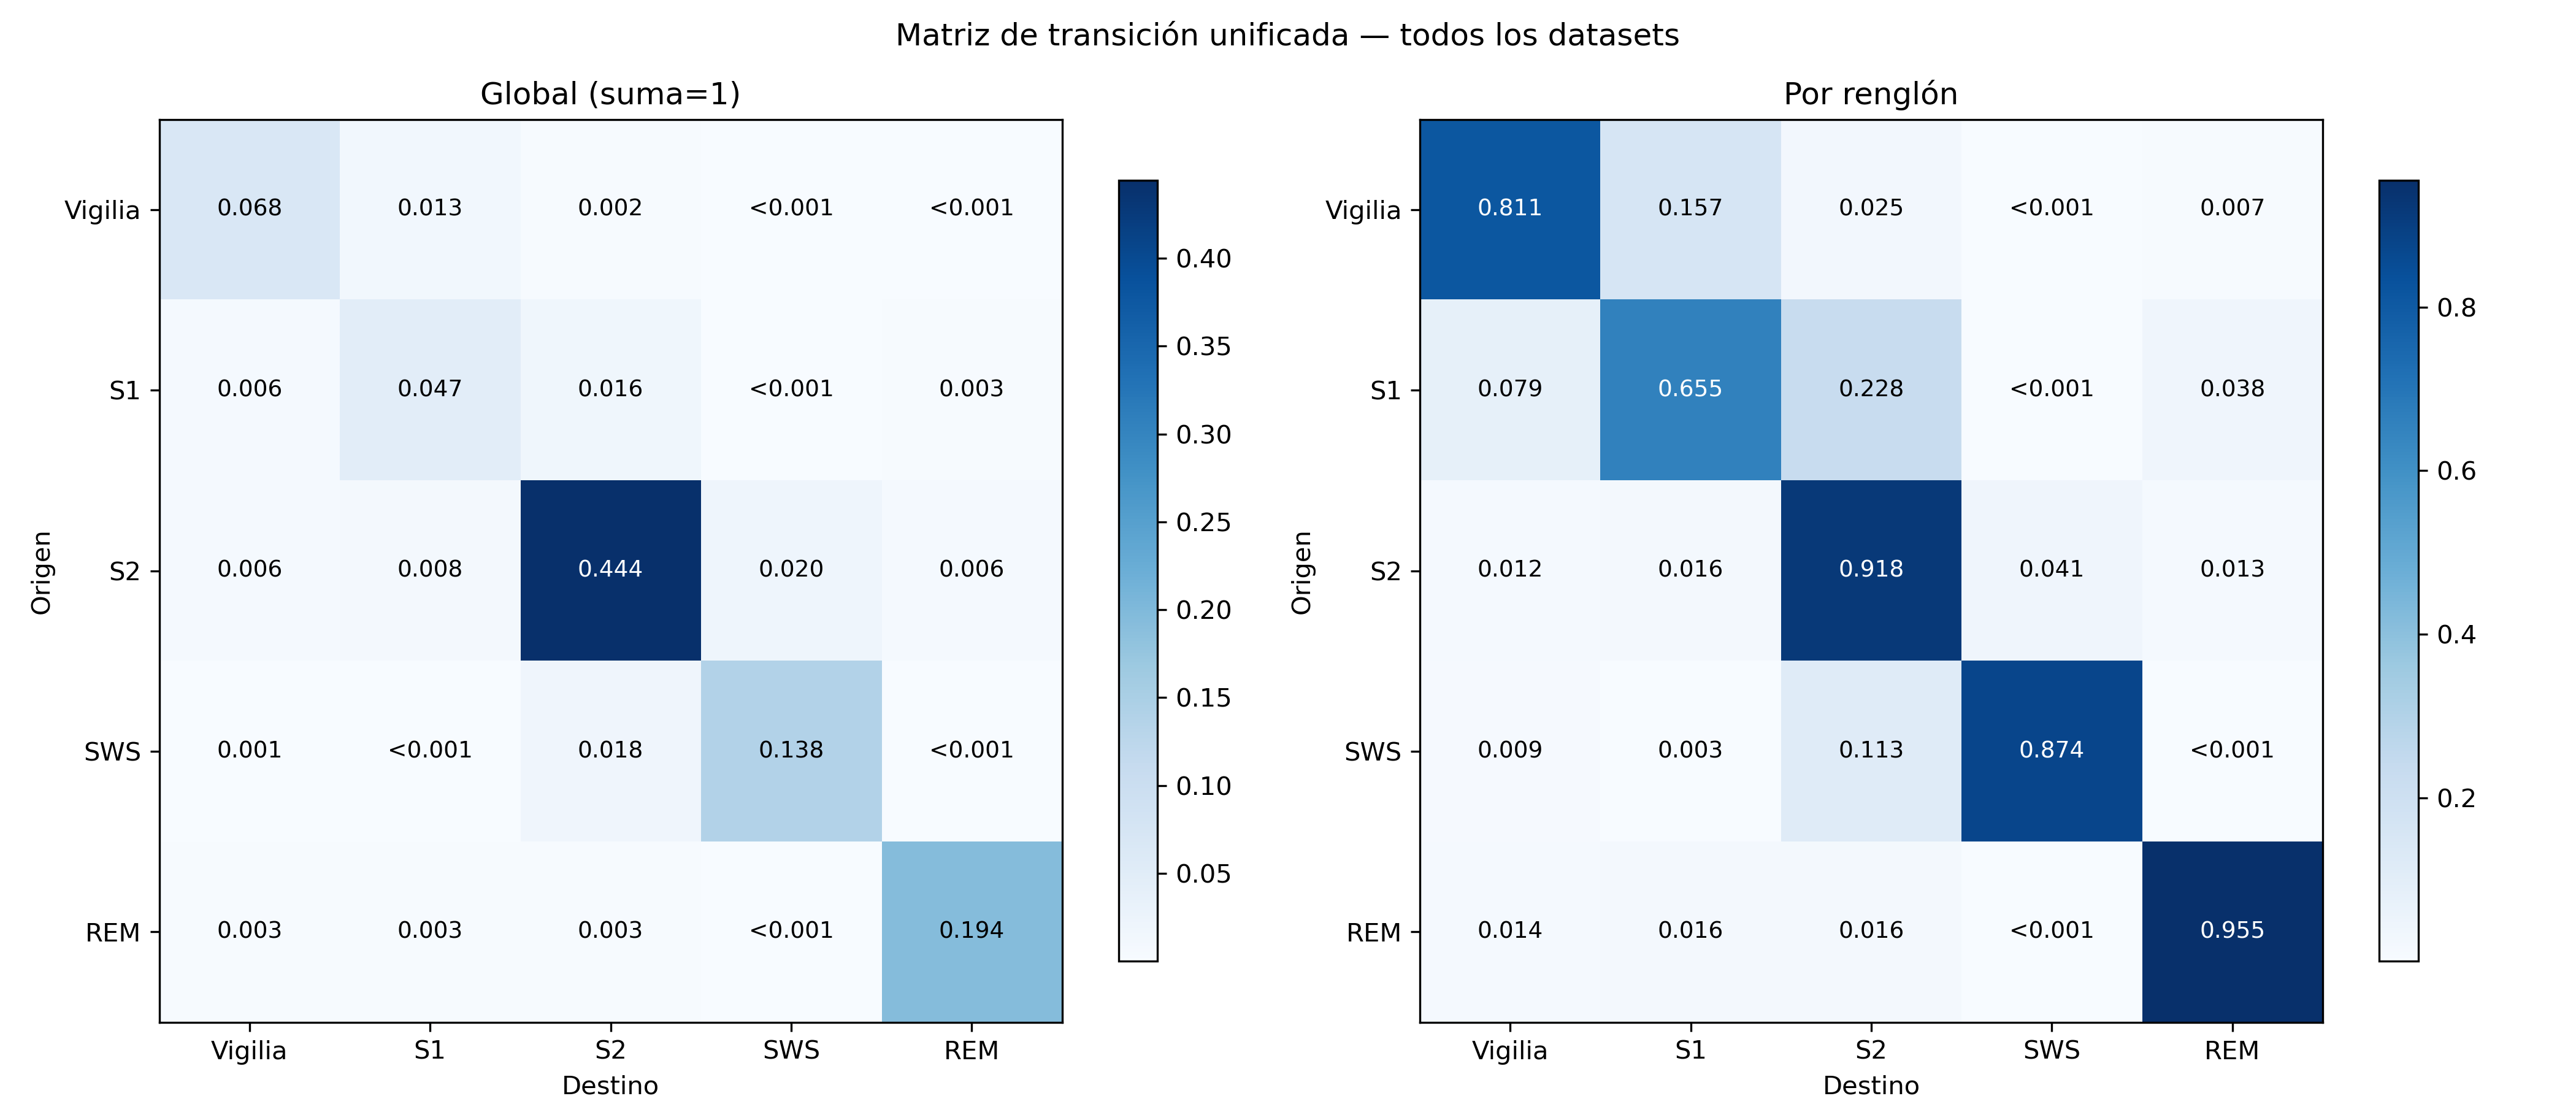
\includegraphics[width=0.95\textwidth]{matriz_transicion_unificada.png}
    \caption{Matriz de Transición Unificada (bigramas, 127 sujetos). Izquierda: normalización global. Derecha: normalización por renglón ($P(j|i)$). La diagonal principal de la matriz por renglón exhibe valores elevados (0.65--0.95), indicando alta estabilidad intra-fase. Las celdas fuera de la diagonal revelan las rutas de transición preferentes.}
    \label{fig:matriz_global}
\end{figure}

\subsubsection{Hallazgo Principal: Alta Inercia de Estado}

El resultado más evidente es la \textbf{dominancia diagonal}: una vez que el cerebro entra en una fase, tiende a permanecer en ella. Los valores de la diagonal principal de la matriz por renglón cuantifican esta \textit{inercia}:

\begin{table}[htbp]
\centering
\caption{Probabilidad de permanencia (diagonal) por fase del sueño.}
\label{tab:diagonal_global}
\begin{tabular}{lcc}
\hline
\textbf{Fase} & \textbf{$P(i|i)$} & \textbf{Interpretación} \\
\hline
Vigilia (W) & 0.811 & Alta, pero menor que sueño \\
S1 & 0.655 & Inestable (fase de transición) \\
S2 & 0.918 & Alta estabilidad \\
SWS & 0.874 & Alta estabilidad \\
REM & 0.955 & Máxima estabilidad \\
\hline
\end{tabular}
\end{table}

\textbf{Interpretación fisiológica:} La fase S1 muestra la menor estabilidad (65.5\%), confirmando su rol como estado transitorio entre la vigilia y el sueño consolidado. En contraste, el REM exhibe la máxima inercia (95.5\%), lo cual es consistente con la necesidad biológica de mantener este estado para completar los procesos de consolidación de memoria.

\subsection{Análisis de Transiciones: La Matriz Sin Diagonal}

Para revelar \textit{hacia dónde se dirige} el cerebro cuando decide abandonar una fase, se construyó una versión renormalizada de la matriz donde la diagonal principal es cero. Esto permite analizar las rutas de escape sin que la alta probabilidad de permanencia ``eclipse'' la información.

\subsubsection{Rutas de Escape desde la Fase 2 (S2)}

Al examinar la fila de S2 en la matriz sin diagonal (renormalizada sobre las salidas):
\begin{itemize}
    \item \textbf{50.1\%} transita hacia SWS (Sueño Profundo).
    \item \textbf{19.7\%} transita hacia S1.
    \item \textbf{15.5\%} transita hacia REM.
    \item \textbf{14.7\%} transita hacia Vigilia.
\end{itemize}

\textbf{Conclusión:} La función primaria de la Fase 2 es servir como \textit{puerta de entrada al sueño profundo}. La transición a REM, aunque menos frecuente, representa la ruta alternativa hacia la activación paradójica.

\subsubsection{El Sueño Profundo como ``Callejón Sin Salida''}

Un hallazgo notable emerge de la fila de SWS:
\begin{itemize}
    \item \textbf{89.6\%} de las salidas regresan a S2.
    \item \textbf{0.5\%} transitan directamente a REM (prácticamente nulo).
\end{itemize}

\textbf{Interpretación:} El sueño profundo (SWS) es un ``callejón fisiológico sin salida''. Para abandonarlo, el cerebro debe primero aligerarse hacia S2, respetando la jerarquía de estados. \textit{No existe un atajo SWS $\rightarrow$ REM}; esta restricción topológica valida que los datos corresponden a sueño fisiológico estructurado.

\subsubsection{Inestabilidad Post-REM}

La fila de REM en la matriz sin diagonal revela:
\begin{itemize}
    \item \textbf{34.7\%} regresa a S1.
    \item \textbf{34.5\%} regresa a S2.
    \item \textbf{30.5\%} transita a Vigilia (despertares breves).
\end{itemize}

\textbf{Interpretación:} Aunque el REM es extremadamente estable mientras dura (95.5\% de permanencia), cuando termina, suele hacerlo de manera abrupta, frecuentemente con un breve despertar o un aligeramiento hacia S1, antes de retomar el ciclo descendiendo hacia S2.

\subsection{Evolución de la Estabilidad por Ciclos}

El sueño no es un proceso estacionario; la presión homeostática modula progresivamente la robustez de las fases a lo largo de la noche. Para cuantificar este fenómeno, se calcularon matrices de transición independientes para cada ciclo ultradiano (aproximadamente 90 minutos) sobre el dataset unificado de 127 pacientes. El análisis se concentra en los ciclos 1 a 4, cuya cobertura es del 100\% (ciclo 1) y se mantiene por encima del 87.4\% (ciclo 4); en ciclos más tardíos la muestra se reduce.

La Figura \ref{fig:estabilidad_ciclos} muestra la evolución de la diagonal principal ($P(i|i)$) a través de los ciclos.

\begin{figure}[htbp]
    \centering
    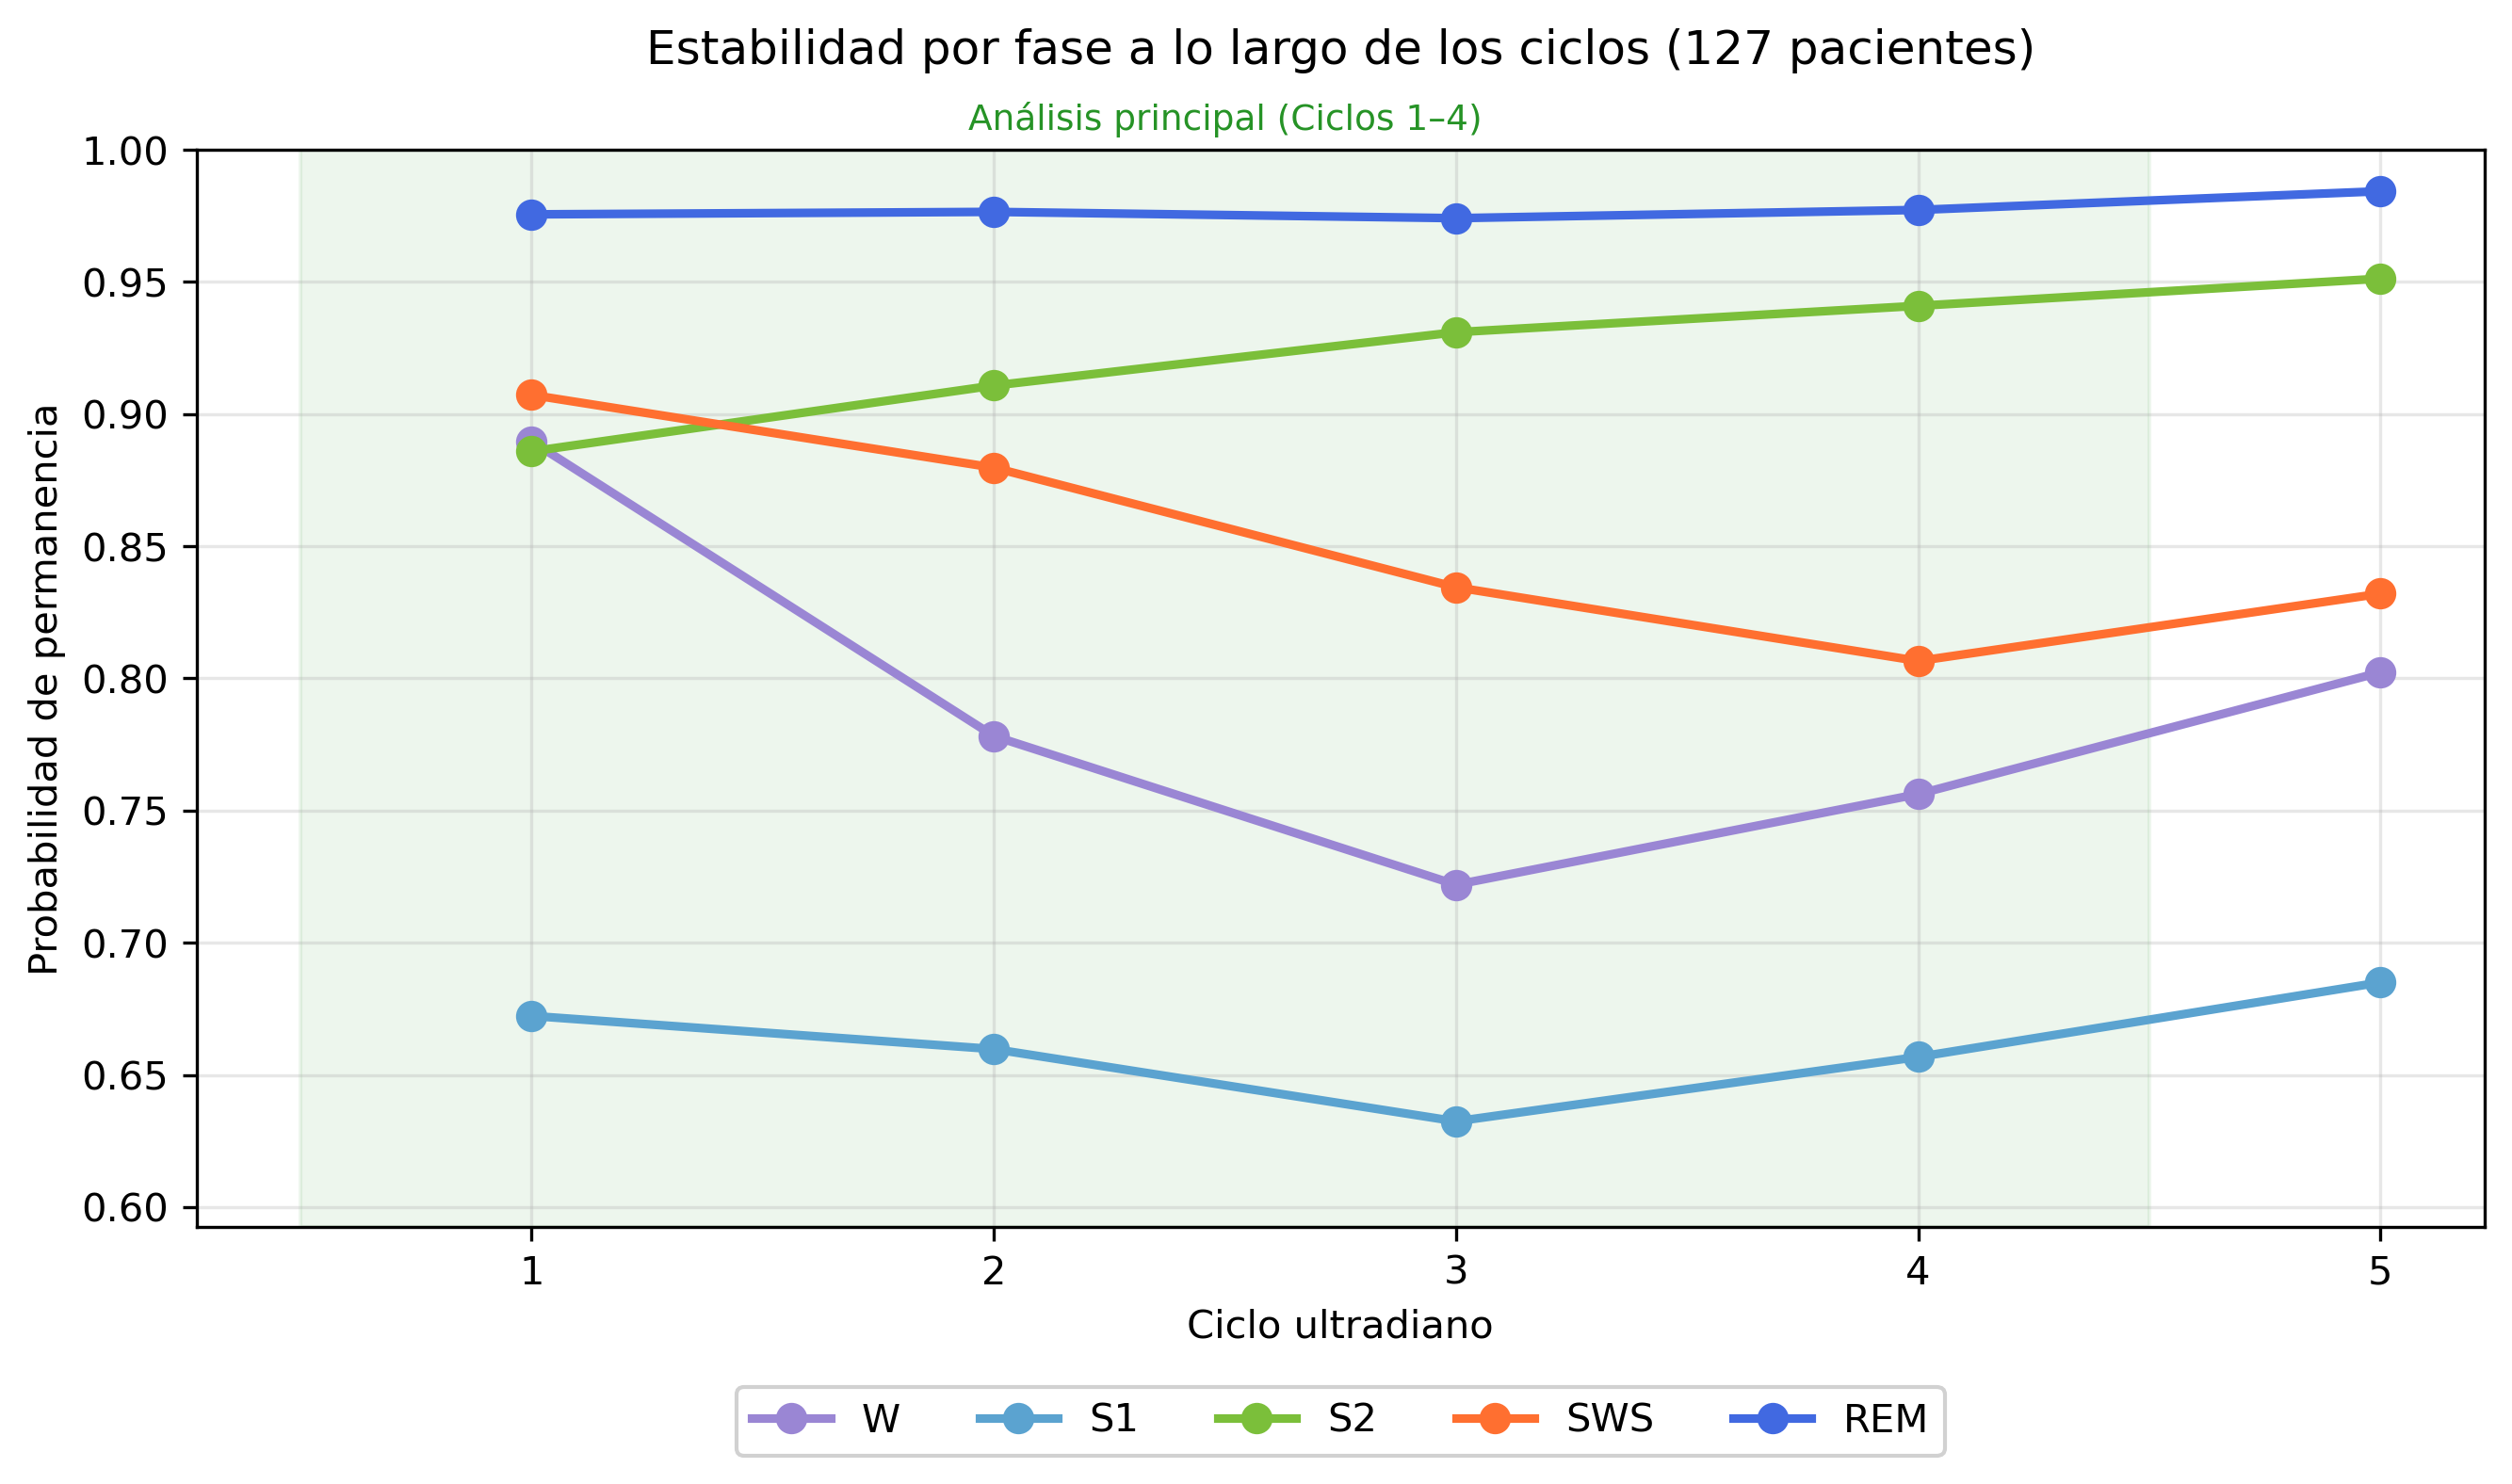
\includegraphics[width=1.0\textwidth]{evolucion_diagonal.png}
    \caption{Evolución de la Estabilidad (Diagonal) por Ciclo, dataset unificado (127 pacientes). El SWS muestra una caída progresiva desde 0.907 (Ciclo 1) hasta 0.807 (Ciclo 4), reflejando la disipación de la presión homeostática, mientras que S2 asciende de forma sostenida.}
    \label{fig:estabilidad_ciclos}
\end{figure}

\subsubsection{Degradación del Sueño Profundo (SWS)}

El hallazgo más notable es la \textbf{caída de estabilidad del SWS}:
\begin{itemize}
    \item Ciclo 1: $P(\text{SWS}|\text{SWS}) = 0.907$ (máxima consolidación).
    \item Ciclo 3: $P(\text{SWS}|\text{SWS}) = 0.834$ (fragmentación emergente).
    \item Ciclo 4: $P(\text{SWS}|\text{SWS}) = 0.807$ (degradación).
\end{itemize}

Esta curva descendente es una manifestación directa del \textbf{Modelo de Borbély} \cite{borbely1982two}: la presión de sueño (Proceso S) se disipa con cada ciclo de sueño profundo, resultando en episodios de SWS cada vez más breves y frágiles.

\subsubsection{Estabilización de S2}

En contraste con el SWS, la Fase 2 muestra una \textbf{tendencia ascendente}:
\begin{itemize}
    \item Ciclo 1: $P(\text{S2}|\text{S2}) = 0.886$.
    \item Ciclo 4: $P(\text{S2}|\text{S2}) = 0.941$.
    \item Ciclo 5: $P(\text{S2}|\text{S2}) = 0.951$.
\end{itemize}

\textbf{Interpretación:} Conforme el SWS pierde presencia en los ciclos tardíos, S2 se convierte en el ``estado por defecto'' del sueño NREM, ocupando mayor porcentaje del tiempo y mostrando mayor resistencia al cambio.

\subsection{Evolución de las Transiciones desde S2}

Para complementar el análisis de estabilidad, se examinó cómo cambian las \textit{rutas de escape} desde S2 a lo largo de la noche. La Figura \ref{fig:trans_s2_condiag} muestra esta evolución y la Figura \ref{fig:trans_s2_sindiag} la contrasta por dataset.

\begin{figure}[htbp]
    \centering
    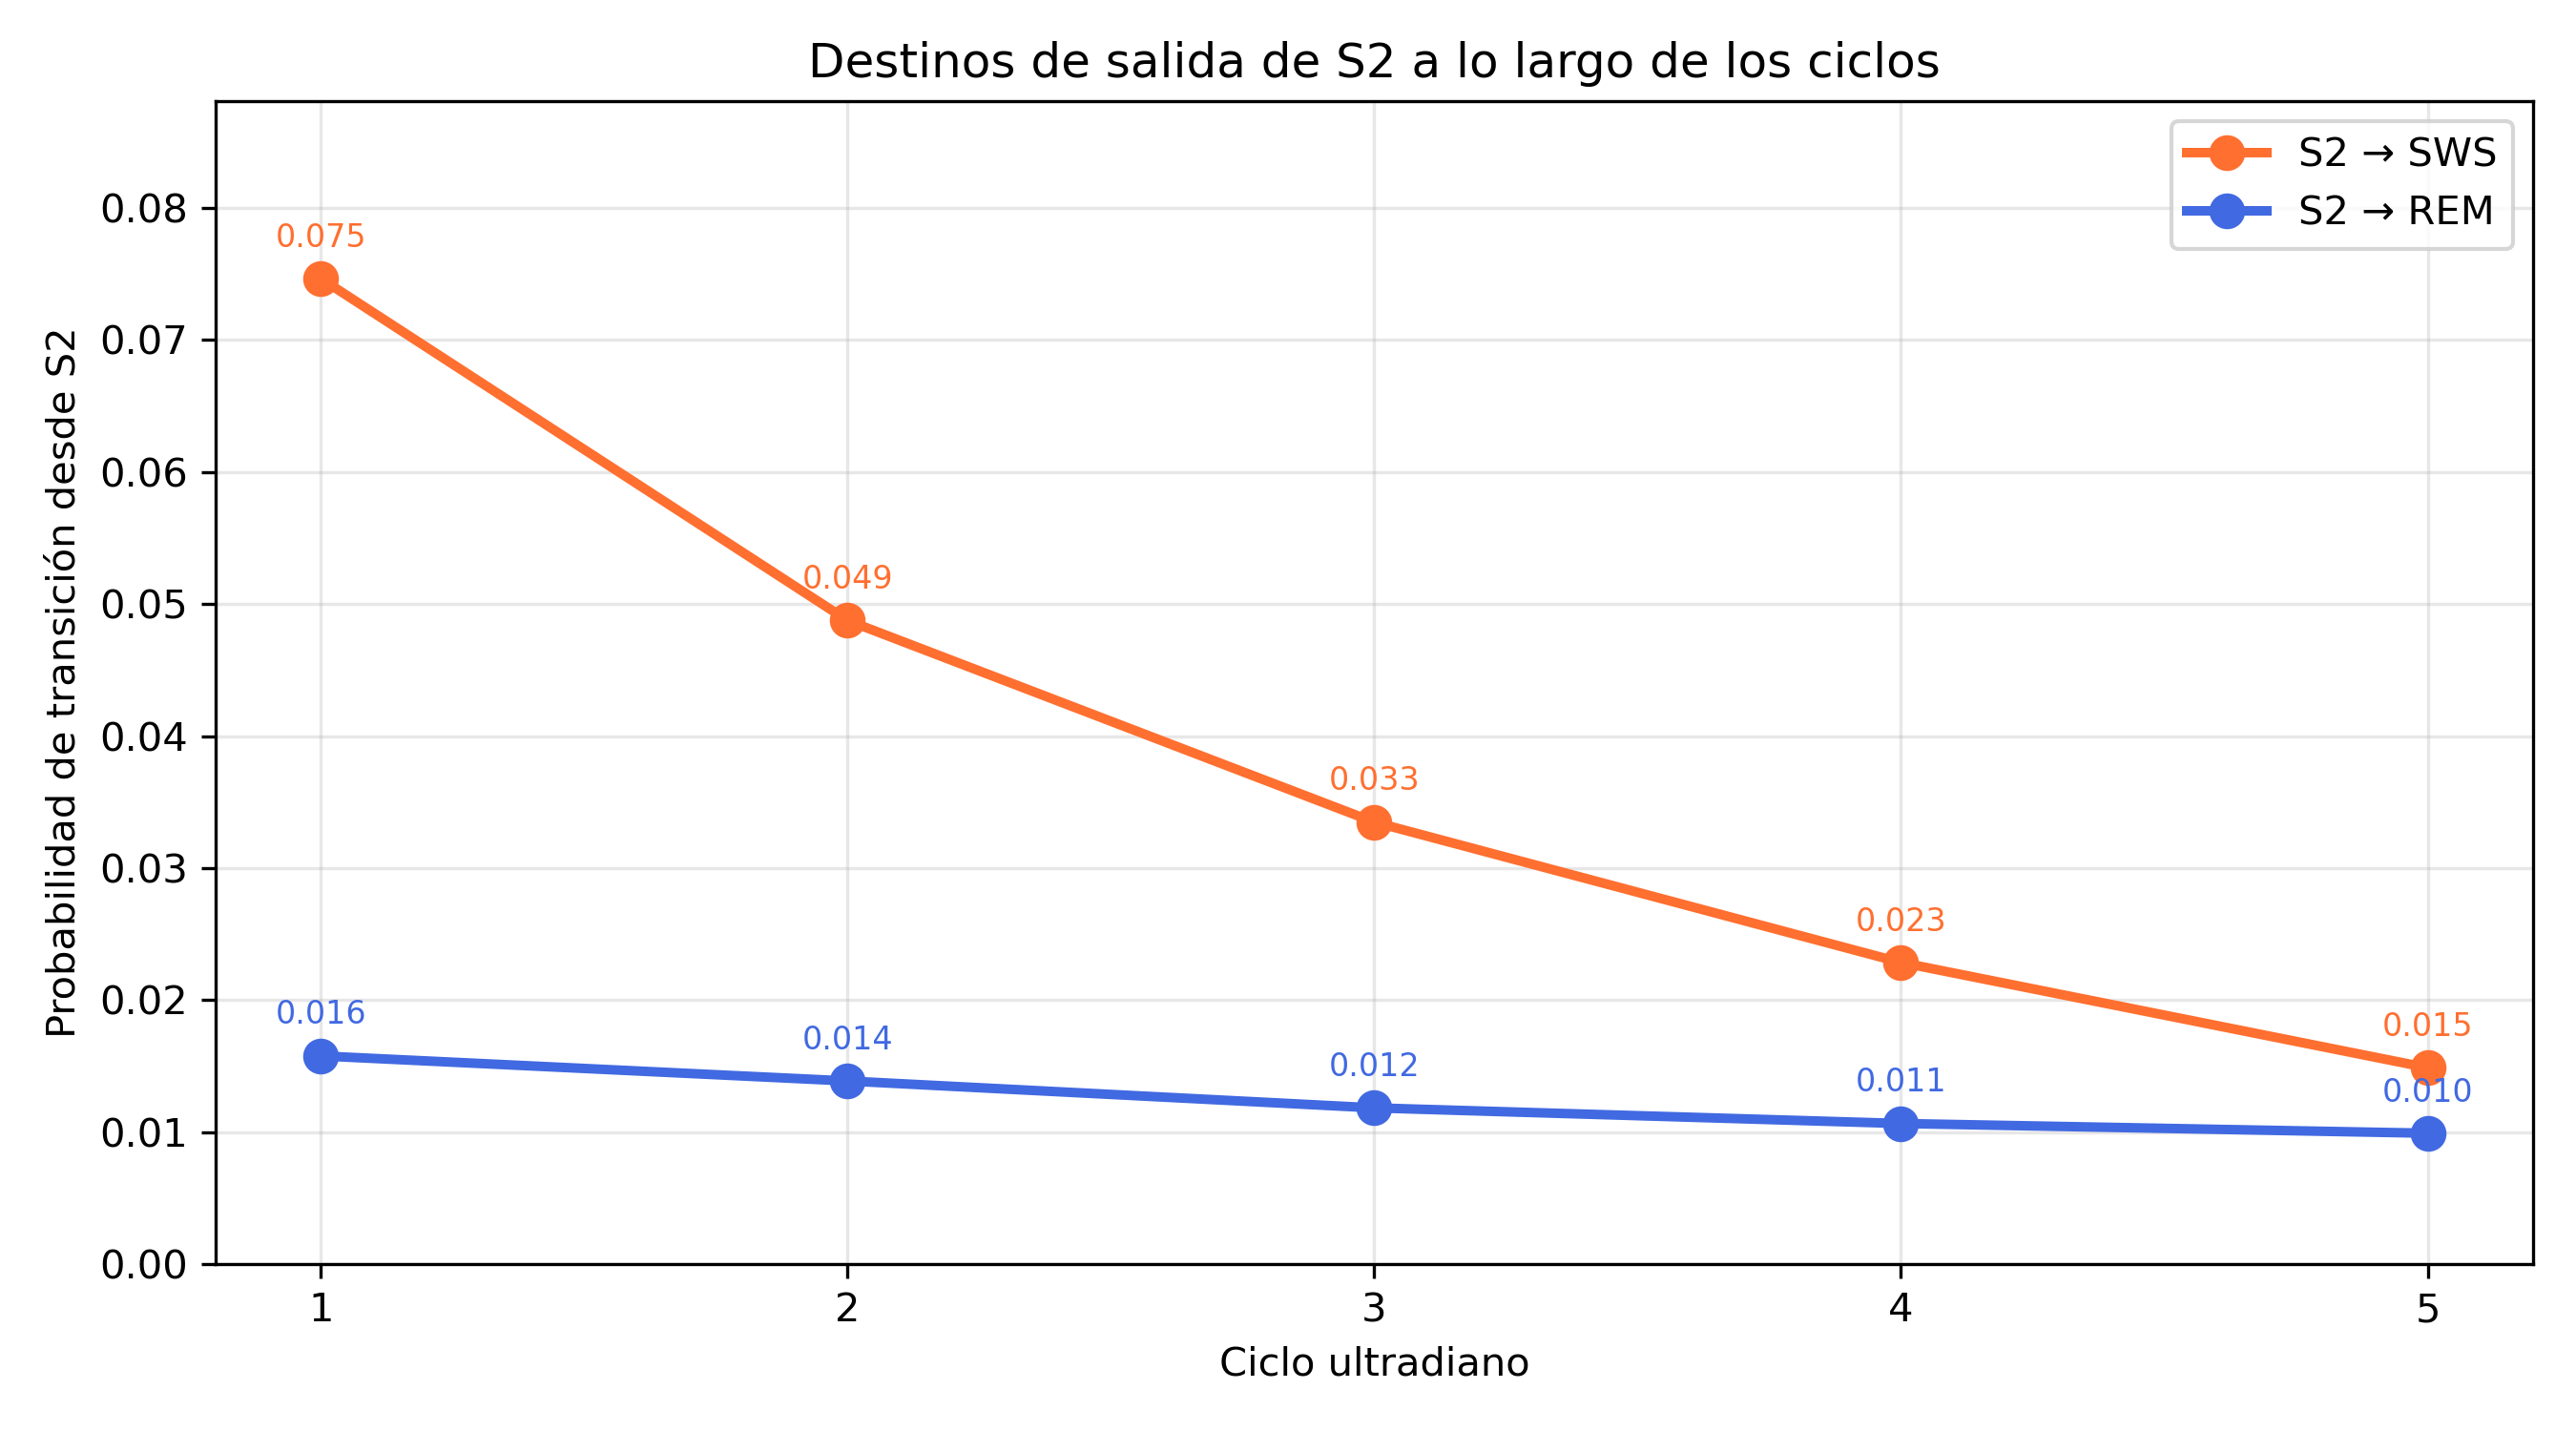
\includegraphics[width=1.0\textwidth]{evolucion_s2_destinos.png}
    \caption{Evolución de los destinos de S2 a lo largo de los ciclos (dataset unificado, ciclos 1--5). La probabilidad $P(\text{S2} \rightarrow \text{SWS})$ cae drásticamente del Ciclo 1 al 5, mientras que $P(\text{S2} \rightarrow \text{REM})$ permanece relativamente constante.}
    \label{fig:trans_s2_condiag}
\end{figure}

\begin{figure}[htbp]
    \centering
    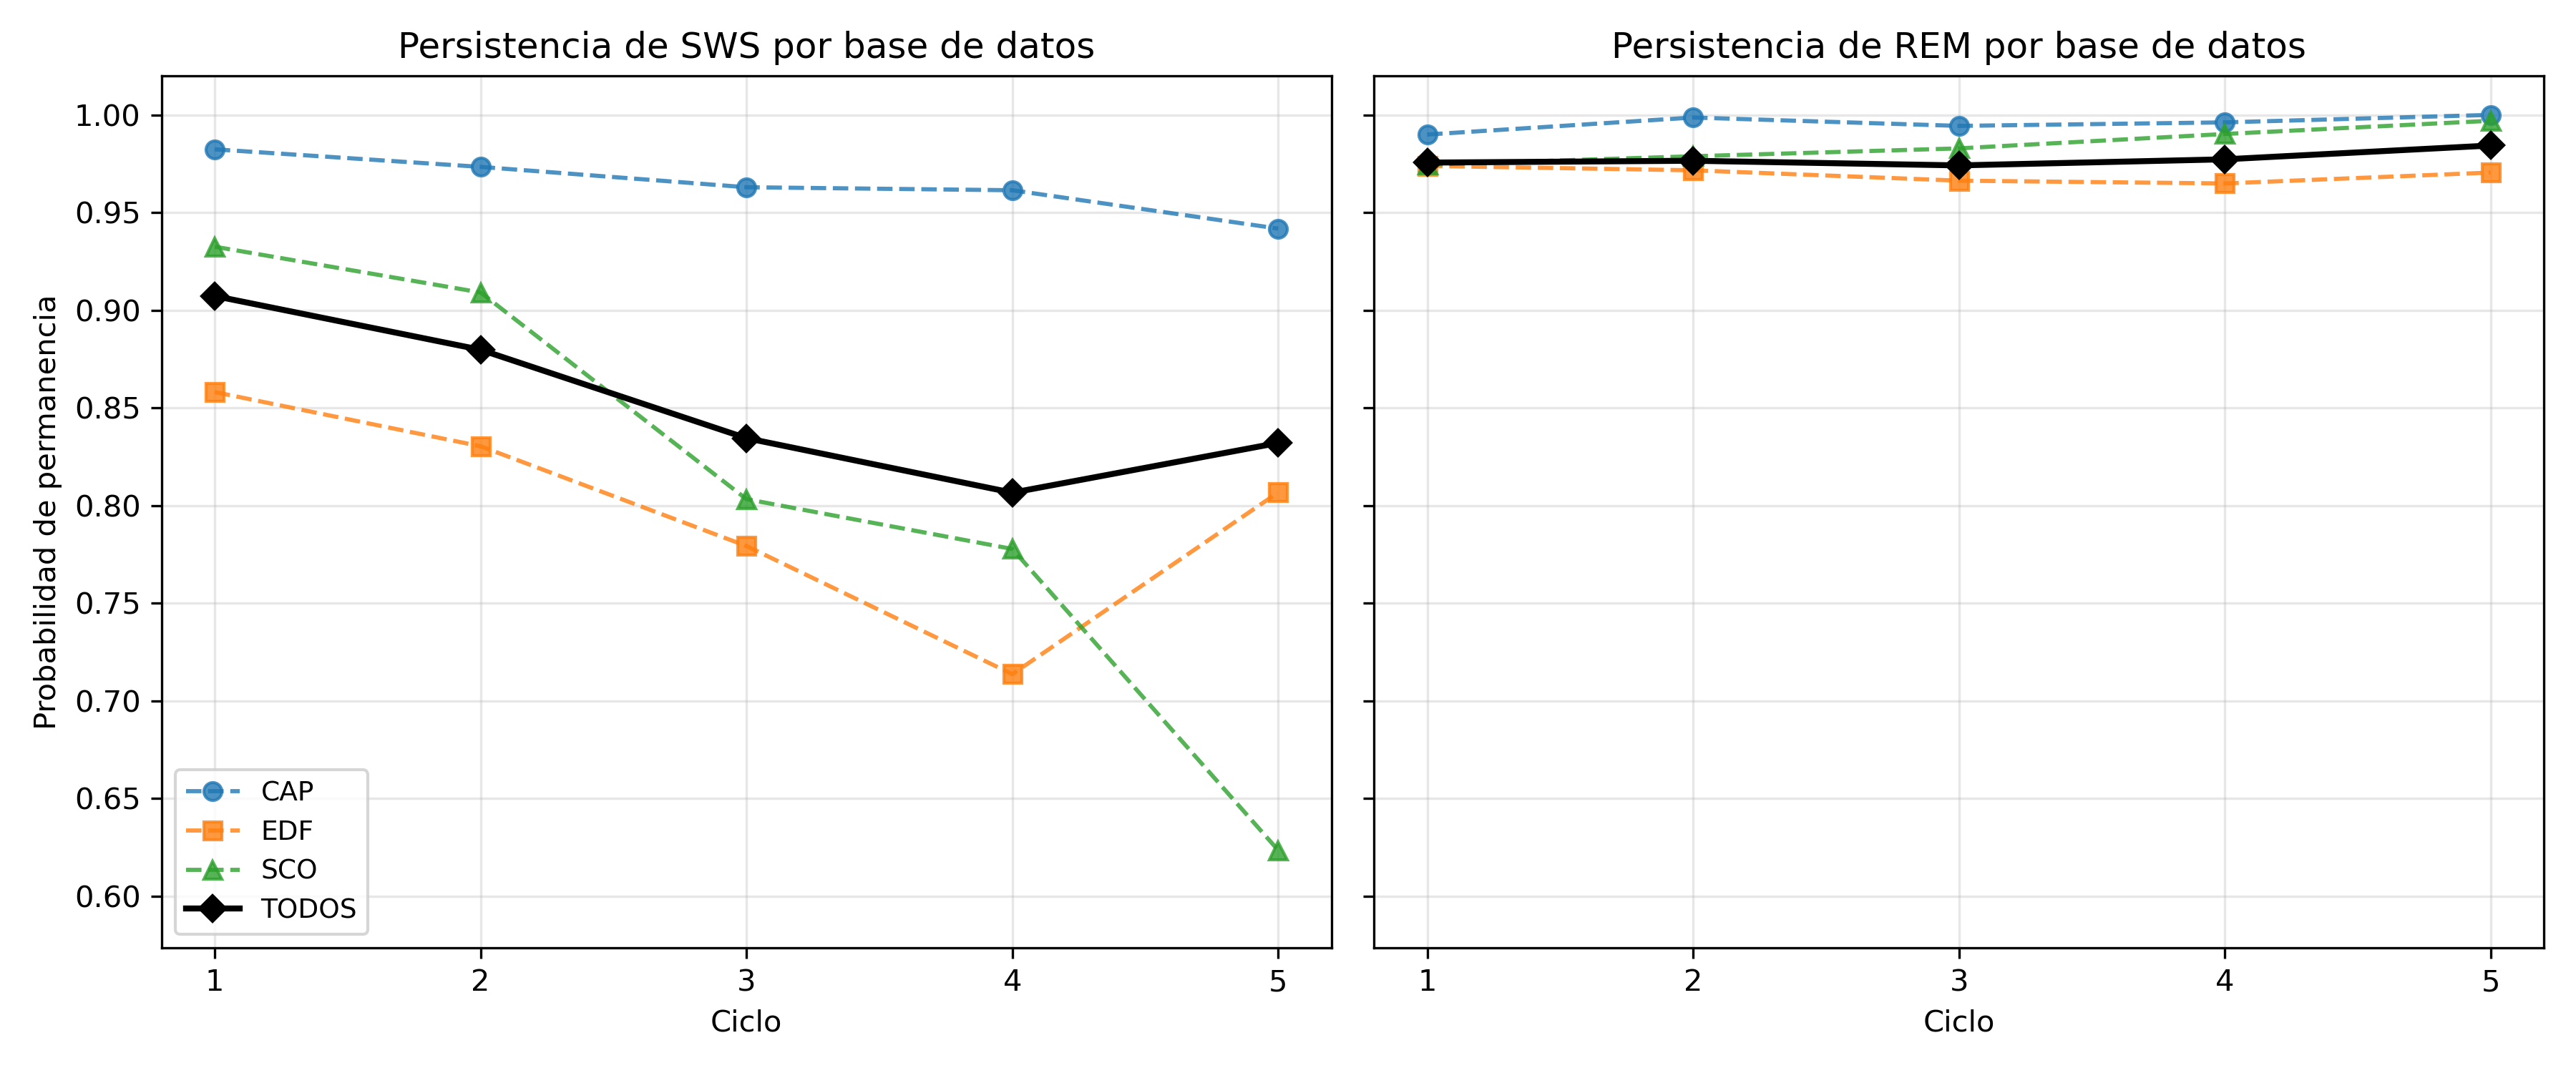
\includegraphics[width=1.0\textwidth]{comparativo_sws_rem_por_dataset.png}
    \caption{Persistencia de SWS y REM por ciclo, desagregada por dataset (CAP, EDF, SCO). La tendencia descendente del SWS y la mayor estabilidad del REM son consistentes entre las tres fuentes, validando que el patrón no depende de un dataset particular.}
    \label{fig:trans_s2_sindiag}
\end{figure}

\textbf{Hallazgo clave:} La probabilidad de transitar de S2 a SWS cae de 0.0746 (Ciclo 1) a 0.0149 (Ciclo 5), una reducción del 80\%. En el mismo intervalo, la transición $\text{S2} \rightarrow \text{REM}$ se mantiene prácticamente constante (de 0.0158 a 0.0099). Este resultado cuantifica matemáticamente la ``escasez de sueño profundo'' en las últimas horas de la noche.

\subsection{Conclusión del Análisis Markoviano}

El análisis de Cadenas de Markov respalda la \textbf{Hipótesis H1 (Estructural)}: el sueño sano no es un proceso aleatorio, sino que posee una estructura no fragmentada. En concreto:
\begin{enumerate}
    \item \textbf{El sueño es estable y estructurado:} Las fases exhiben alta inercia y las transiciones respetan la topología fisiológica (no hay atajos SWS $\rightarrow$ REM).
    \item \textbf{El sueño se degrada con la noche:} La estabilidad del SWS decae exponencialmente, mientras que S2 se consolida como estado dominante.
    \item \textbf{S2 es un distribuidor central:} Actúa como nodo de paso obligado entre el sueño ligero, el sueño profundo y el REM.
\end{enumerate}

Sin embargo, este análisis markoviano tiene una \textbf{limitación fundamental}: asume que las probabilidades de transición son constantes dentro de cada fase. La pregunta que motiva la siguiente sección es: ¿Existe una escala temporal óptima para analizar las transiciones que capture la micro-dinámica oculta dentro de cada época?

\section{Determinación de la Escala Temporal: Criterio Multi-Objetivo}

El análisis markoviano anterior demostró que el sueño es un proceso estable con transiciones estructuradas. Sin embargo, Markov asume tiempos de permanencia fijos (distribución geométrica). Para abordar la \textbf{Hipótesis H2 (Lingüística)} ---que los hipnogramas pueden tratarse como secuencias simbólicas con propiedades análogas a las de un lenguaje natural---, buscamos la escala de tokenización $N$ que produzca el mejor compromiso entre estructura tipo lenguaje, calidad del ajuste y cobertura de los bloques de Fase 2.

\subsection{Análisis Global: Cola Pesada en la Duración de S2}

Al analizar la distribución de duración de los bloques continuos de S2 sobre la noche completa, los datos exhiben una \textbf{distribución de cola pesada}. Sobre los 4 437 bloques de S2 del dataset unificado, la duración media es de 12.10 épocas pero la mediana es de apenas 5 épocas, con un percentil 90 de 34 épocas: existen segmentos de S2 que duran desde 30 segundos hasta más de 15 minutos, sin una escala característica única.

Este comportamiento confirma que, a nivel global, el sueño carece de una duración ``típica'' para la Fase 2, y que la media está fuertemente sesgada por los bloques largos. Esto invalida metodológicamente el uso de una ventana basada en el promedio global: necesitamos un criterio de selección más robusto.

\subsection{Exploración Matemática: El Barrido de N-gramas}

Para buscar estructura, realizamos un barrido sistemático de n-gramas sobre un amplio rango de escalas ($N$ desde 1 hasta 100 épocas). En cada escala calculamos la distribución rango-frecuencia y su ajuste a una Ley de Zipf \cite{zipf1949human}, cuya pendiente característica $\beta \approx 1$ (en valor absoluto del exponente en escala log-log) señala la eficiencia informativa propia de los lenguajes naturales.

\textbf{¿Por qué la ley de Zipf?} En cualquier idioma humano, si ordenamos las palabras de la más usada a la menos usada, la frecuencia de cada una cae siguiendo una regla muy precisa: la segunda palabra más común aparece la mitad de veces que la primera, la tercera un tercio, y así sucesivamente. Esa regularidad ---la ley de Zipf, con exponente cercano a 1--- no es un capricho estadístico: es la huella de un sistema que reparte la información de forma eficiente, combinando unos pocos elementos muy frecuentes con muchos elementos raros pero específicos. La pregunta que nos hacemos es directa: si troceamos el hipnograma en ``palabras'' de $N$ épocas, ¿esas palabras se distribuyen como las de un idioma? Si la respuesta es sí, entonces el sueño no es una sucesión aleatoria de etapas, sino una secuencia con gramática. El barrido busca, por tanto, la longitud de ``palabra'' $N$ a la que el sueño se parece más a un lenguaje.

La Tabla \ref{tab:barrido_ngramas} resume los hallazgos cuantitativos sobre la cohorte de 127 pacientes sanos:

\begin{table}[htbp]
\centering
\caption{Resultados del barrido de n-gramas: exponente de Zipf y calidad del ajuste.}
\label{tab:barrido_ngramas}
\begin{tabular*}{\textwidth}{@{\extracolsep{\fill}}rrrrl}
\hline
$N$ & Tiempo & $\beta$ & $R^2$ & Interpretación \\
\hline
1 & 30s & 1.195 & 0.980 & Fragmentación alta \\
2 & 1 min & 2.836 & 0.802 & Ley de potencia abrupta \\
5 & 2.5 min & 1.853 & 0.966 & Perfil supra-Zipfiano \\
\textbf{6} & \textbf{3 min} & \textbf{1.597} & \textbf{0.977} & \textbf{Mejor compromiso global} \\
8 & 4 min & 1.250 & 0.972 & Cercano a Zipf \\
10 & 5 min & 1.009 & 0.952 & $\beta$ más próximo a 1 \\
15 & 7.5 min & 0.669 & 0.843 & Degradación estadística \\
50 & 25 min & 0.200 & 0.430 & Colapso del ajuste \\
100 & 50 min & 0.059 & 0.172 & Secuencias casi únicas \\
\hline
\end{tabular*}
\end{table}

La Figura \ref{fig:leypotencia_6} muestra la rejilla de distribuciones frecuencia--rango en escala log-log para distintos valores de $N$, y la Figura \ref{fig:beta_vs_n} traza la evolución del exponente $\beta$ en función de $N$.

\begin{figure}[htbp]
    \centering
    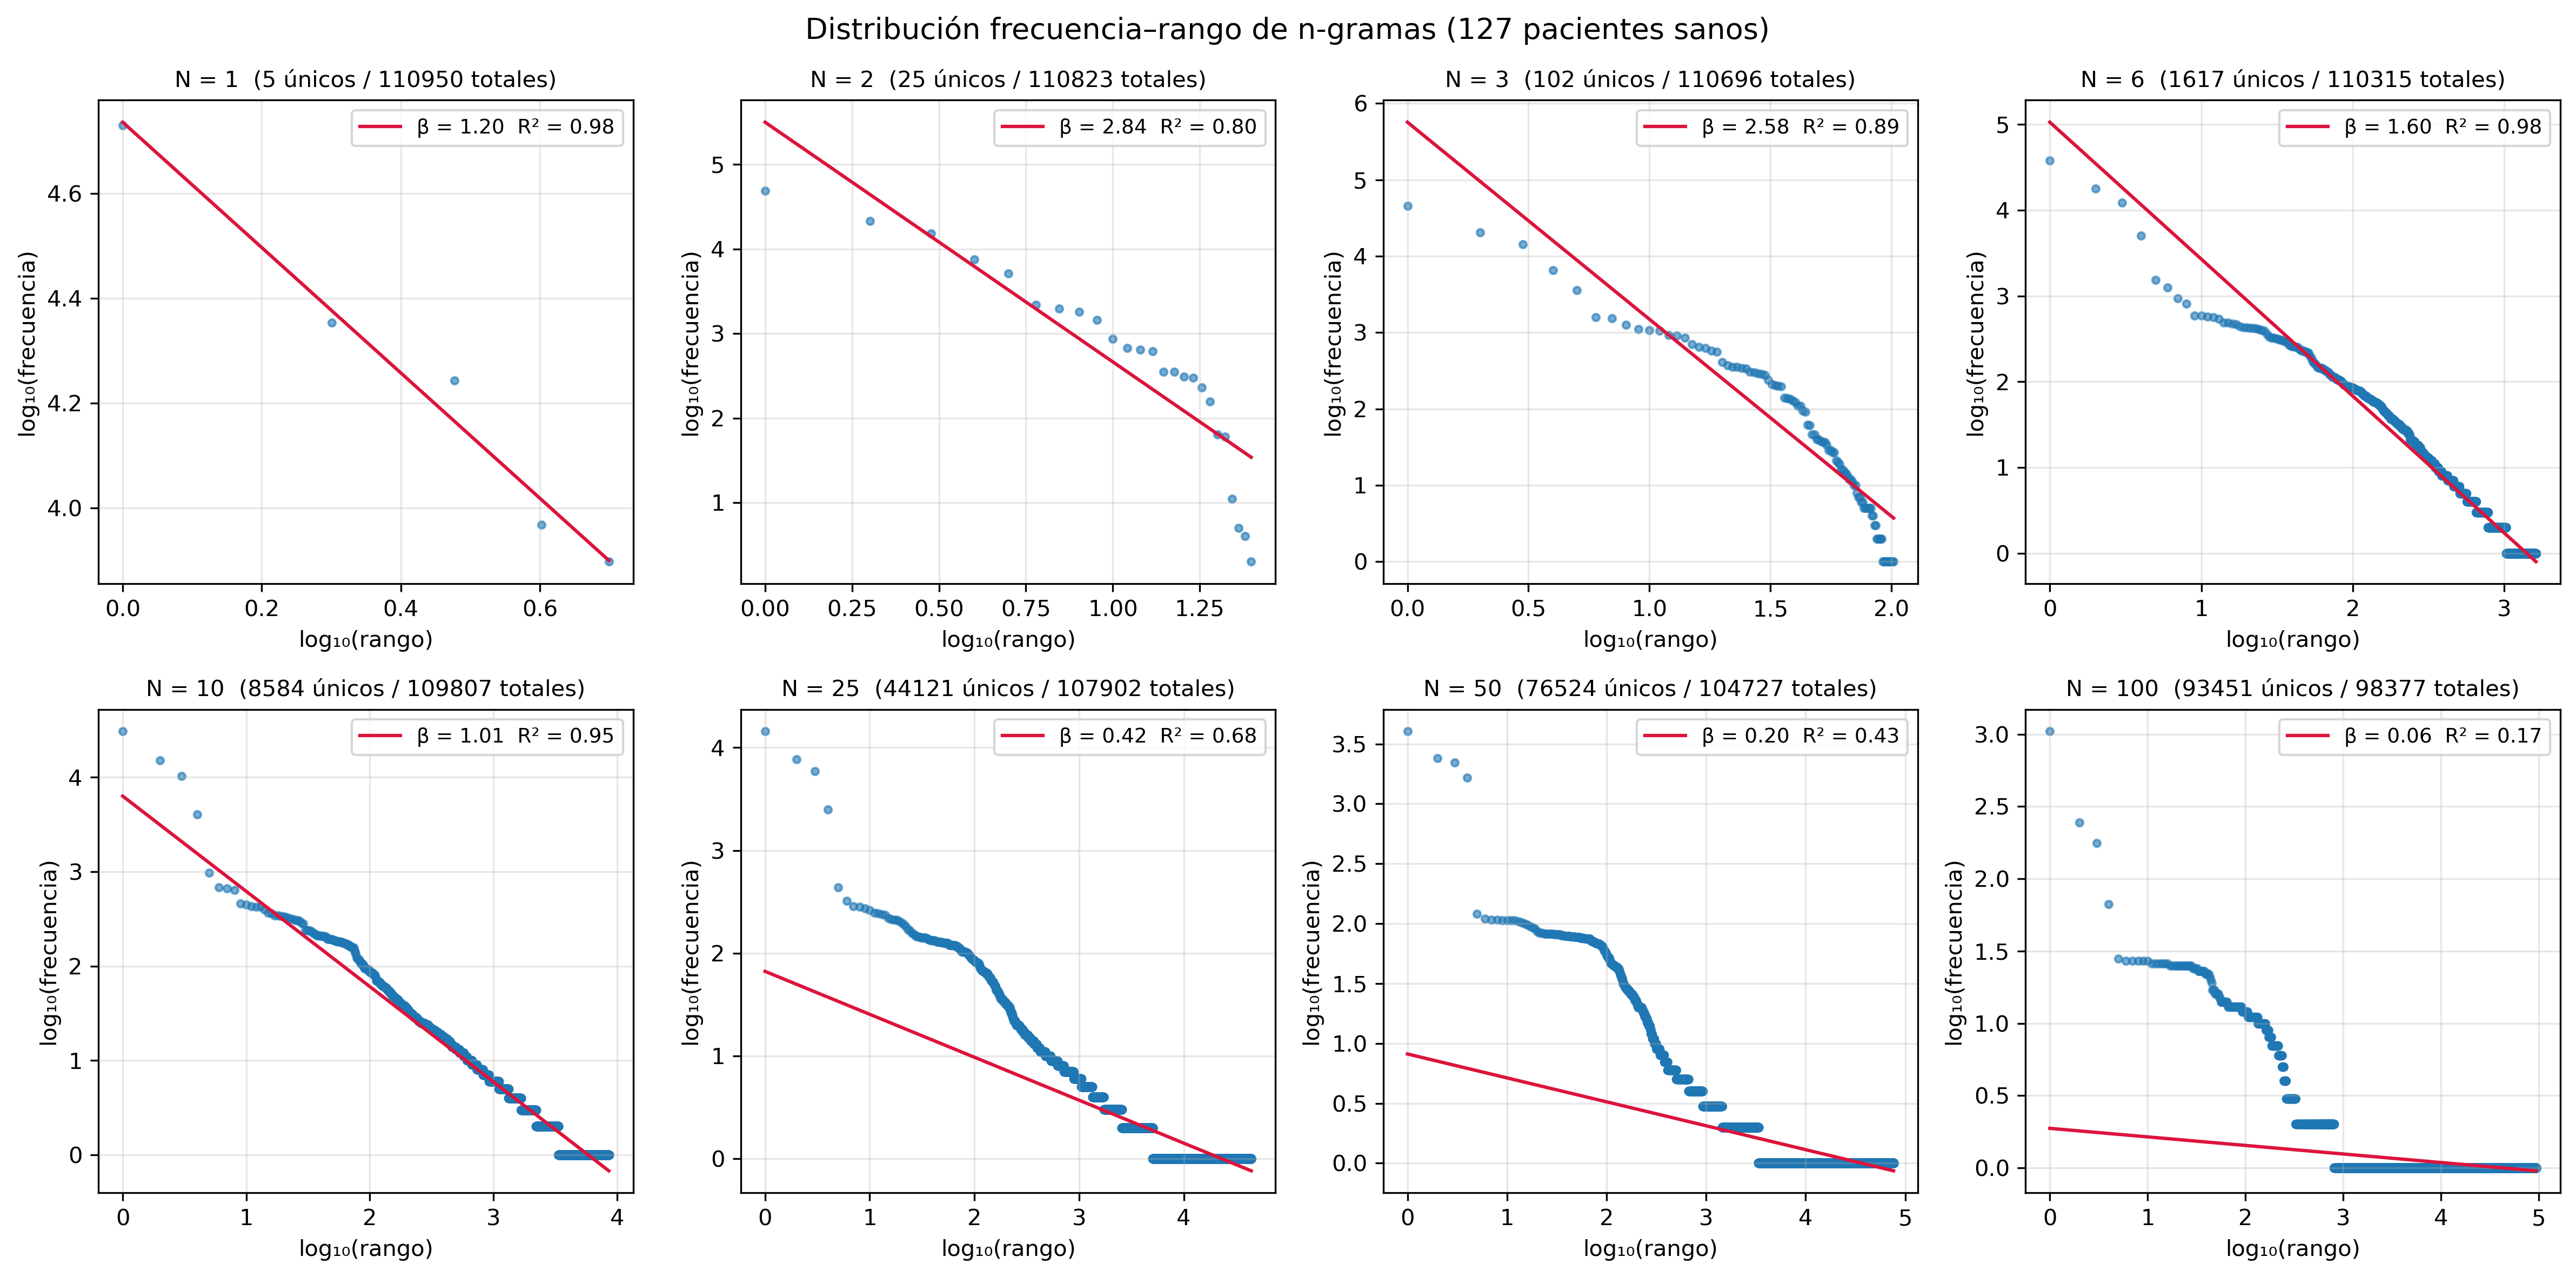
\includegraphics[width=1.0\textwidth]{zipf_loglog_grid.png}
    \caption{Distribución frecuencia--rango de n-gramas en escala log-log (127 pacientes sanos) para varios valores de $N$. La linealidad es máxima en las escalas intermedias, donde la distribución se aproxima a una Ley de Zipf.}
    \label{fig:leypotencia_6}
\end{figure}

\begin{figure}[htbp]
    \centering
    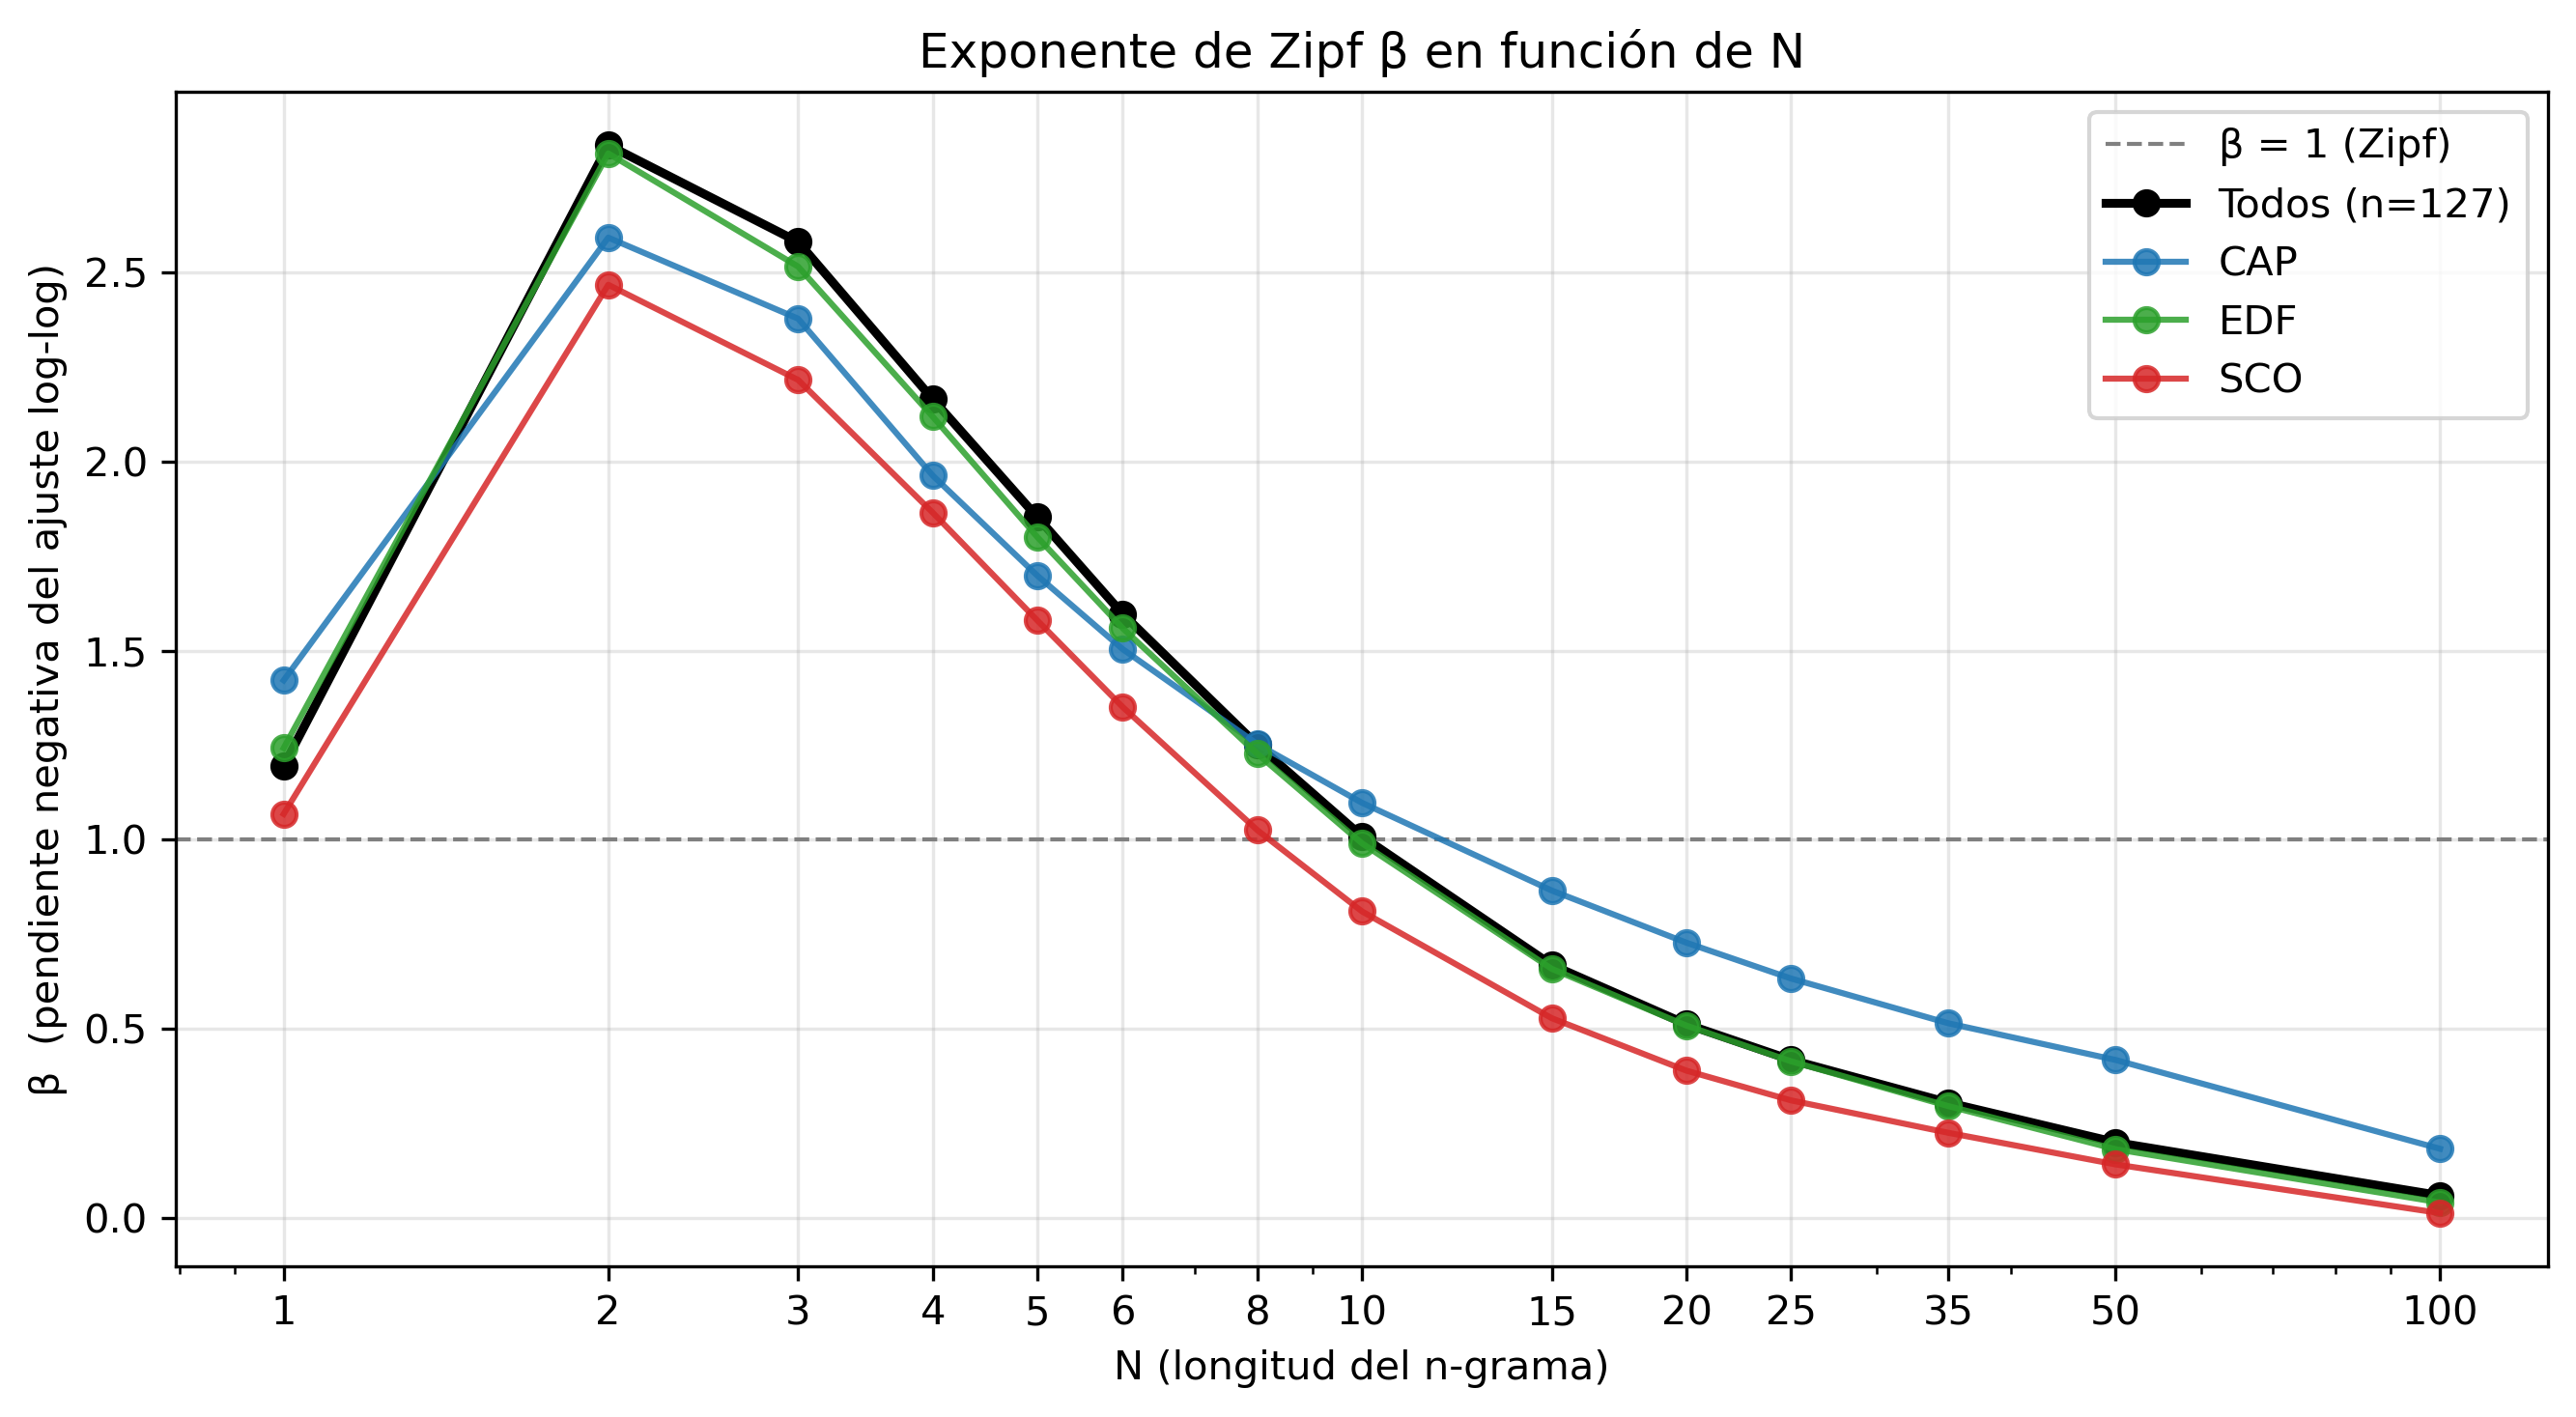
\includegraphics[width=0.9\textwidth]{zipf_beta_vs_n.png}
    \caption{Exponente de Zipf $\beta$ en función de $N$. El exponente decrece monótonamente con la longitud del n-grama y cruza el valor de referencia $\beta=1$ entre $N=8$ ($\beta=1.250$) y $N=10$ ($\beta=1.009$).}
    \label{fig:beta_vs_n}
\end{figure}

\textbf{Matiz honesto:} El exponente $\beta$ decrece de forma continua con $N$, de modo que el valor más cercano a la referencia $\beta=1$ se alcanza en $N=10$ ($\beta=1.009$), no en $N=6$. Sin embargo, $\beta$ por sí solo no basta como criterio: a medida que crece $N$, la calidad del ajuste ($R^2$) y la cobertura de los bloques de S2 se deterioran. Por ello, la elección de $N$ no puede reducirse a minimizar $|\beta-1|$. Conviene además ser cauto con la interpretación: un buen ajuste lineal en escala log-log es \textit{compatible} con una ley de potencia, pero no constituye una prueba formal de ella (otras distribuciones de cola pesada producen rectas similares en rangos acotados). Por eso, a lo largo del texto hablamos de distribución \textit{compatible} con la ley de Zipf y no de una ley de potencia demostrada.

\subsection{Selección Multi-Criterio de N}

Un solo número puede engañar. Si nos guiáramos únicamente por el exponente $\beta$, elegiríamos la escala donde el sueño ``parece'' más un idioma; pero ese parecido podría ser una ilusión si los datos en realidad no se alinean bien, o si la escala es tan grande que cada ``palabra'' aparece una única vez en toda la noche y, por tanto, no describe nada reutilizable. Por eso evaluamos cada candidato $N$ con \textbf{tres preguntas complementarias}, cada una de las cuales vigila un punto ciego de las otras dos:

\begin{enumerate}
    \item \textbf{¿Se parece a un lenguaje?} ---Proximidad a Zipf, medida como $|\beta - 1|$. Cuanto más cerca está el exponente de 1, más se ajusta la distribución de n-gramas al reparto eficiente de información típico de un idioma.
    \item \textbf{¿Es confiable ese parecido?} ---Calidad del ajuste, el coeficiente $R^2$ de la regresión log-log. Un $\beta$ ideal no significa nada si la nube de puntos no cae realmente sobre una recta; $R^2$ mide cuán sólida es la ley y descarta coincidencias espurias.
    \item \textbf{¿Describe el sueño real?} ---Cobertura, el porcentaje de épocas de S2 que quedan contenidas en bloques de longitud $\geq N$. A medida que $N$ crece, las ``palabras'' se vuelven tan específicas que casi no se repiten (se convierten en \textit{hápax}) y dejan de representar el sueño efectivo; la cobertura penaliza esa fragmentación.
\end{enumerate}

La clave es que estos tres criterios están \textbf{en tensión}: al alargar la ventana $N$, el exponente $\beta$ mejora y se acerca a 1 (el sueño ``suena'' más a idioma), pero simultáneamente se degradan el ajuste $R^2$ y la cobertura, porque las secuencias largas se vuelven únicas. Al acortarla ocurre lo contrario: cobertura altísima, pero un $\beta$ demasiado pronunciado. No existe un $N$ que gane en los tres a la vez, así que la decisión honesta no es maximizar una métrica, sino \textbf{buscar el mejor equilibrio}. Para ello traducimos cada criterio a una posición en un \textit{ranking} sobre los candidatos y promediamos las tres posiciones (menor es mejor).

\begin{table}[htbp]
\centering
\caption{Selección multi-criterio de $N$. El \textit{score} medio promedia los tres rankings; menor es mejor.}
\label{tab:seleccion_N}
\begin{tabular*}{\textwidth}{@{\extracolsep{\fill}}rrrrrr}
\hline
$N$ & $\beta$ & $R^2$ & Cobertura S2 (\%) & \textit{Score} medio & Posición \\
\hline
\textbf{6} & \textbf{1.597} & \textbf{0.977} & \textbf{47.33} & \textbf{3.33} & \textbf{1.\textsuperscript{o}} \\
7 & 1.405 & 0.977 & 44.24 & 3.67 & 2.\textsuperscript{o} \\
8 & 1.250 & 0.972 & 41.00 & 3.67 & 2.\textsuperscript{o} \\
9 & 1.121 & 0.964 & 38.07 & 4.00 & 4.\textsuperscript{o} \\
5 & 1.853 & 0.966 & 51.77 & 4.33 & 5.\textsuperscript{o} \\
10 & 1.009 & 0.952 & 35.99 & 4.33 & 5.\textsuperscript{o} \\
12 & 0.835 & 0.913 & 31.49 & 5.67 & 7.\textsuperscript{o} \\
15 & 0.669 & 0.843 & 25.96 & 7.00 & 8.\textsuperscript{o} \\
\hline
\end{tabular*}
\end{table}

El ganador es \textbf{$N=6$} (\textit{score} medio 3.33): aunque su $\beta$ no es el más cercano a 1, presenta el mejor $R^2$ del barrido (0.977) y conserva una cobertura del 47.33\% de las épocas de S2, logrando el equilibrio más favorable entre los tres objetivos. La Figura \ref{fig:justif_N} integra visualmente estos criterios.

\begin{figure}[htbp]
    \centering
    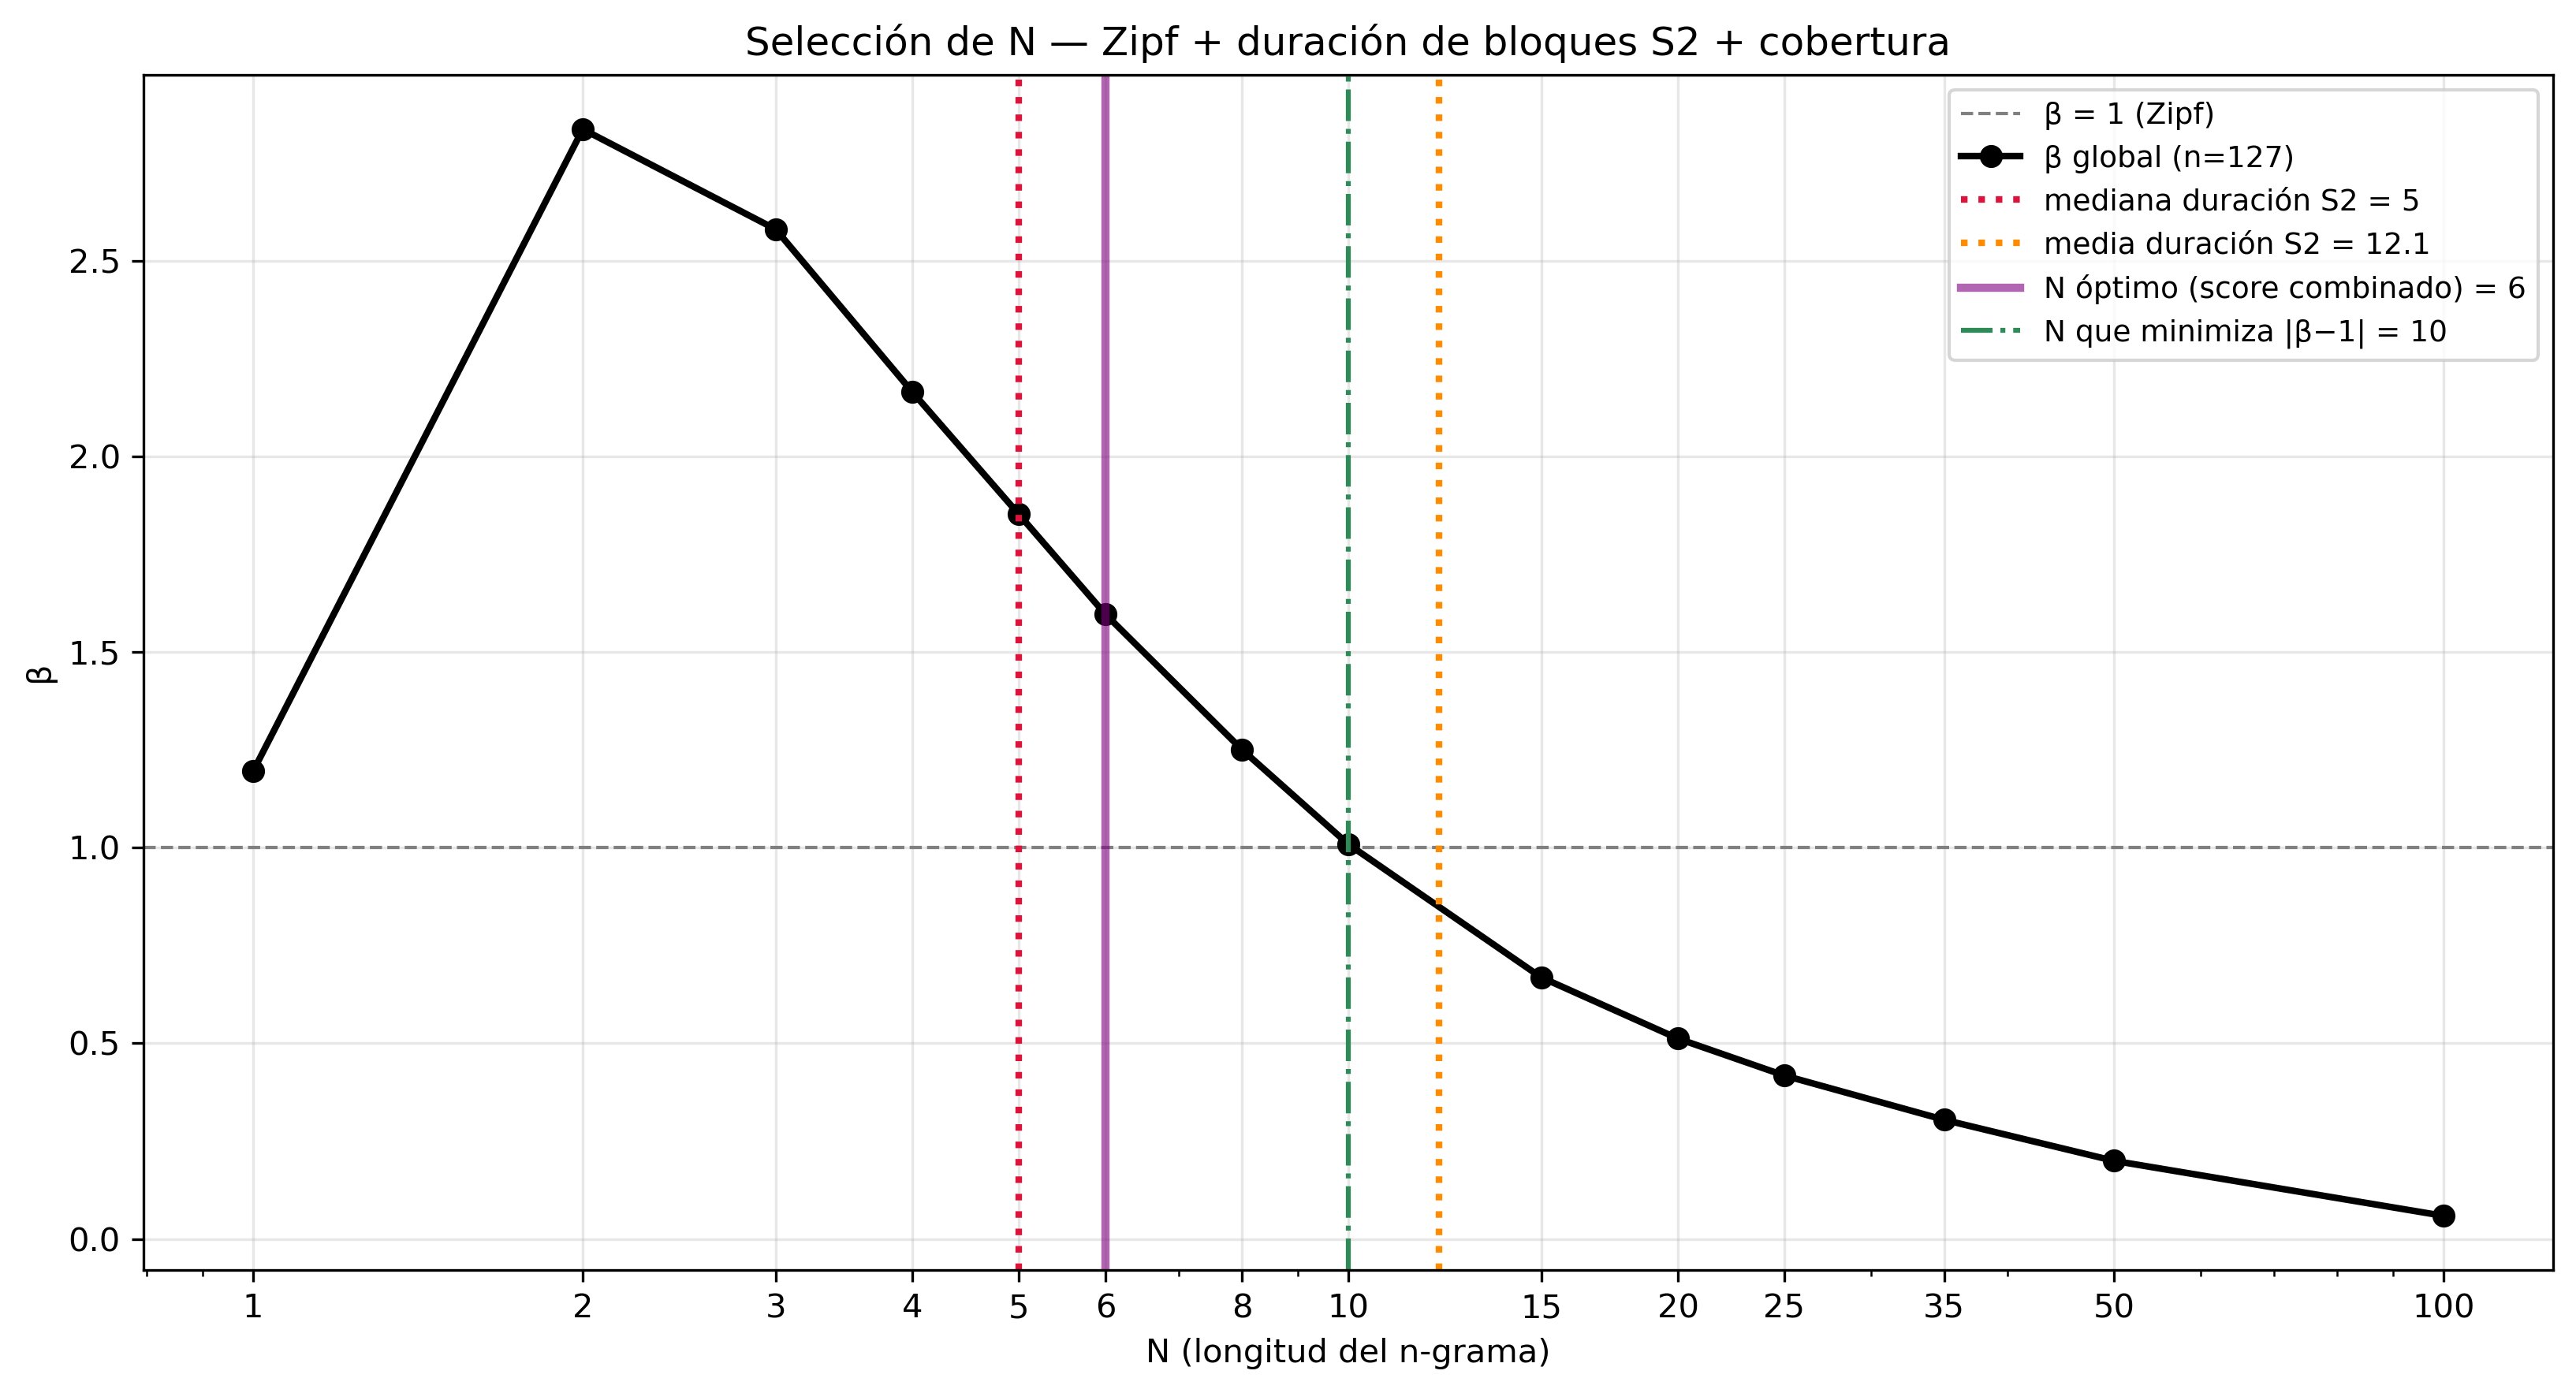
\includegraphics[width=1.0\textwidth]{justificacion_N_combinada.png}
    \caption{Selección de $N$ combinando el exponente de Zipf, la mediana y media de la duración de bloques S2, y la cobertura. La franja señalada corresponde a la región donde convergen los criterios, con $N=6$ como mejor compromiso.}
    \label{fig:justif_N}
\end{figure}

La Figura \ref{fig:ciclo1} presenta el histograma de duración de los bloques de S2 que respalda el criterio de cobertura.

\begin{figure}[htbp]
    \centering
    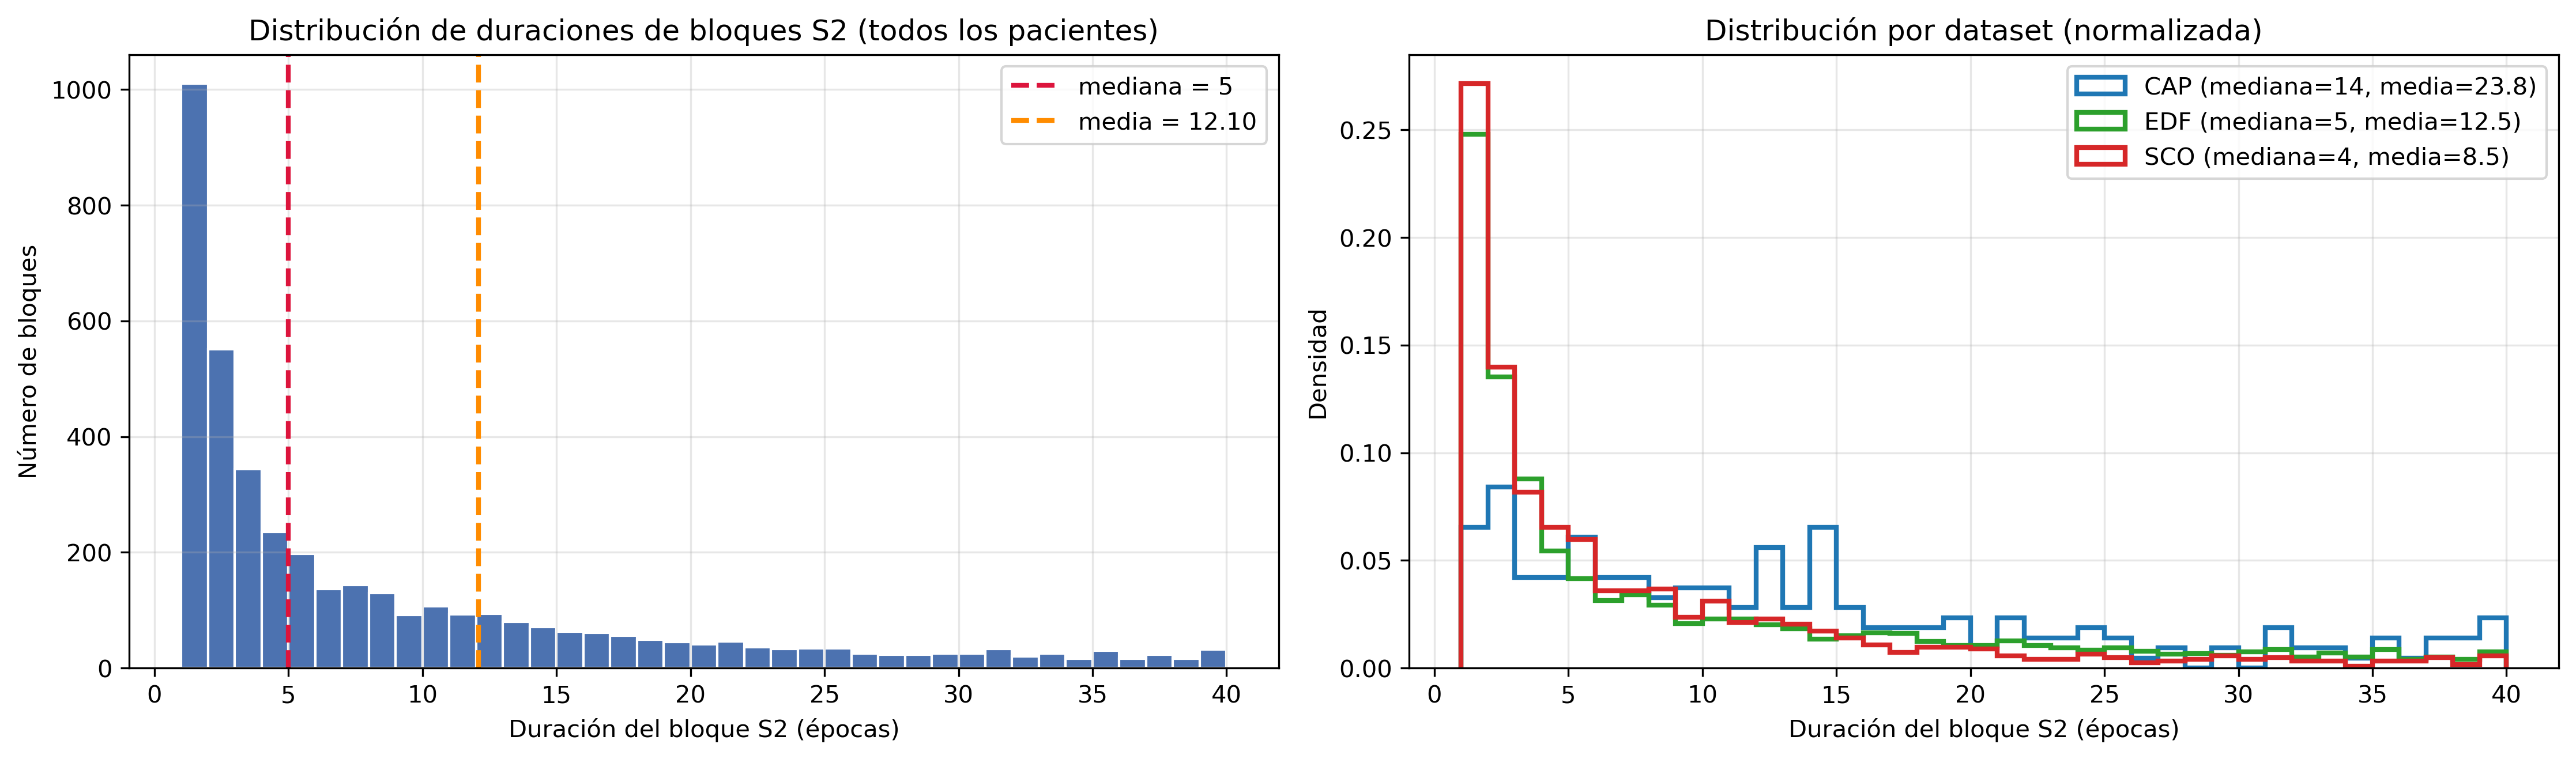
\includegraphics[width=1.0\textwidth]{duracion_s2_histograma.png}
    \caption{Distribución de la duración de los bloques continuos de S2 (todos los pacientes). La mediana (5 épocas) y la media (12.10 épocas) divergen por la cola pesada de la distribución; una ventana de $N=6$ épocas cubre el 47.33\% del tiempo total en S2.}
    \label{fig:ciclo1}
\end{figure}

\subsection{Conclusión: una Escala Justificada, no Arbitraria}

La elección de $N=6$ (3 minutos) no descansa en un único número ni en una coincidencia: emerge del mejor compromiso entre tres criterios cuantitativos independientes evaluados sobre toda la cohorte. Esta escala es la unidad fundamental para el análisis de trayectorias vectoriales de la siguiente sección, y \textbf{apoya la Hipótesis H2 (Lingüística)}: existe una resolución temporal en la que la distribución de n-gramas de sueño es compatible con la organización estadística de un lenguaje natural.

\subsection{Integración con el Análisis Markoviano}

La cola pesada en la duración de S2 explica por qué el análisis markoviano clásico, aunque correcto en sus conclusiones sobre estabilidad y rutas de transición, no puede capturar la dinámica interna de las fases. La distribución geométrica implícita en Markov predice tiempos de permanencia exponencialmente decrecientes, pero los datos reales muestran una cola pesada con eventos de larga duración que ocurren con probabilidad no despreciable. Esta discrepancia justifica incorporar modelos que capturen dependencias de largo plazo mediante representación vectorial (Word2Vec). La ventana $N=6$ será la unidad fundamental para el análisis de trayectorias.

\section{Topología Basal del Espacio Latente: Validación con Unigramas}

Aunque el modelo dinámico opera sobre secuencias complejas de 6 épocas ($N=6$), es fundamental validar primero si el algoritmo ha aprendido correctamente las relaciones entre los \textbf{estados fundamentales} del sueño. Si los ``ladrillos'' básicos (las fases individuales) no están bien posicionados geométricamente en el espacio vectorial, cualquier análisis de secuencias complejas carecería de validez.

Para esta validación topológica, extrajimos los embeddings correspondientes a los \textbf{unigramas} (los tokens unitarios: W, S1, S2, SWS, REM y Sin clasificar) y proyectamos su estructura utilizando UMAP. Esto nos permite visualizar el ``esqueleto'' o la estructura canónica del espacio latente sin el ruido visual que introducirían los 1 503 6-gramas del vocabulario.

\subsection{Proyección UMAP: El Mapa de los Estados Canónicos}

La Figura \ref{fig:umap_unigramas_2d} muestra la disposición espacial de las fases (unigramas) en el espacio vectorial aprendido. A modo de anticipo, la Figura \ref{fig:umap_6g_3d} proyecta además el espacio de 6-gramas en 3D, cuya estructura de trayectorias se analiza en detalle en las secciones siguientes.

\begin{figure}[htbp]
    \centering
    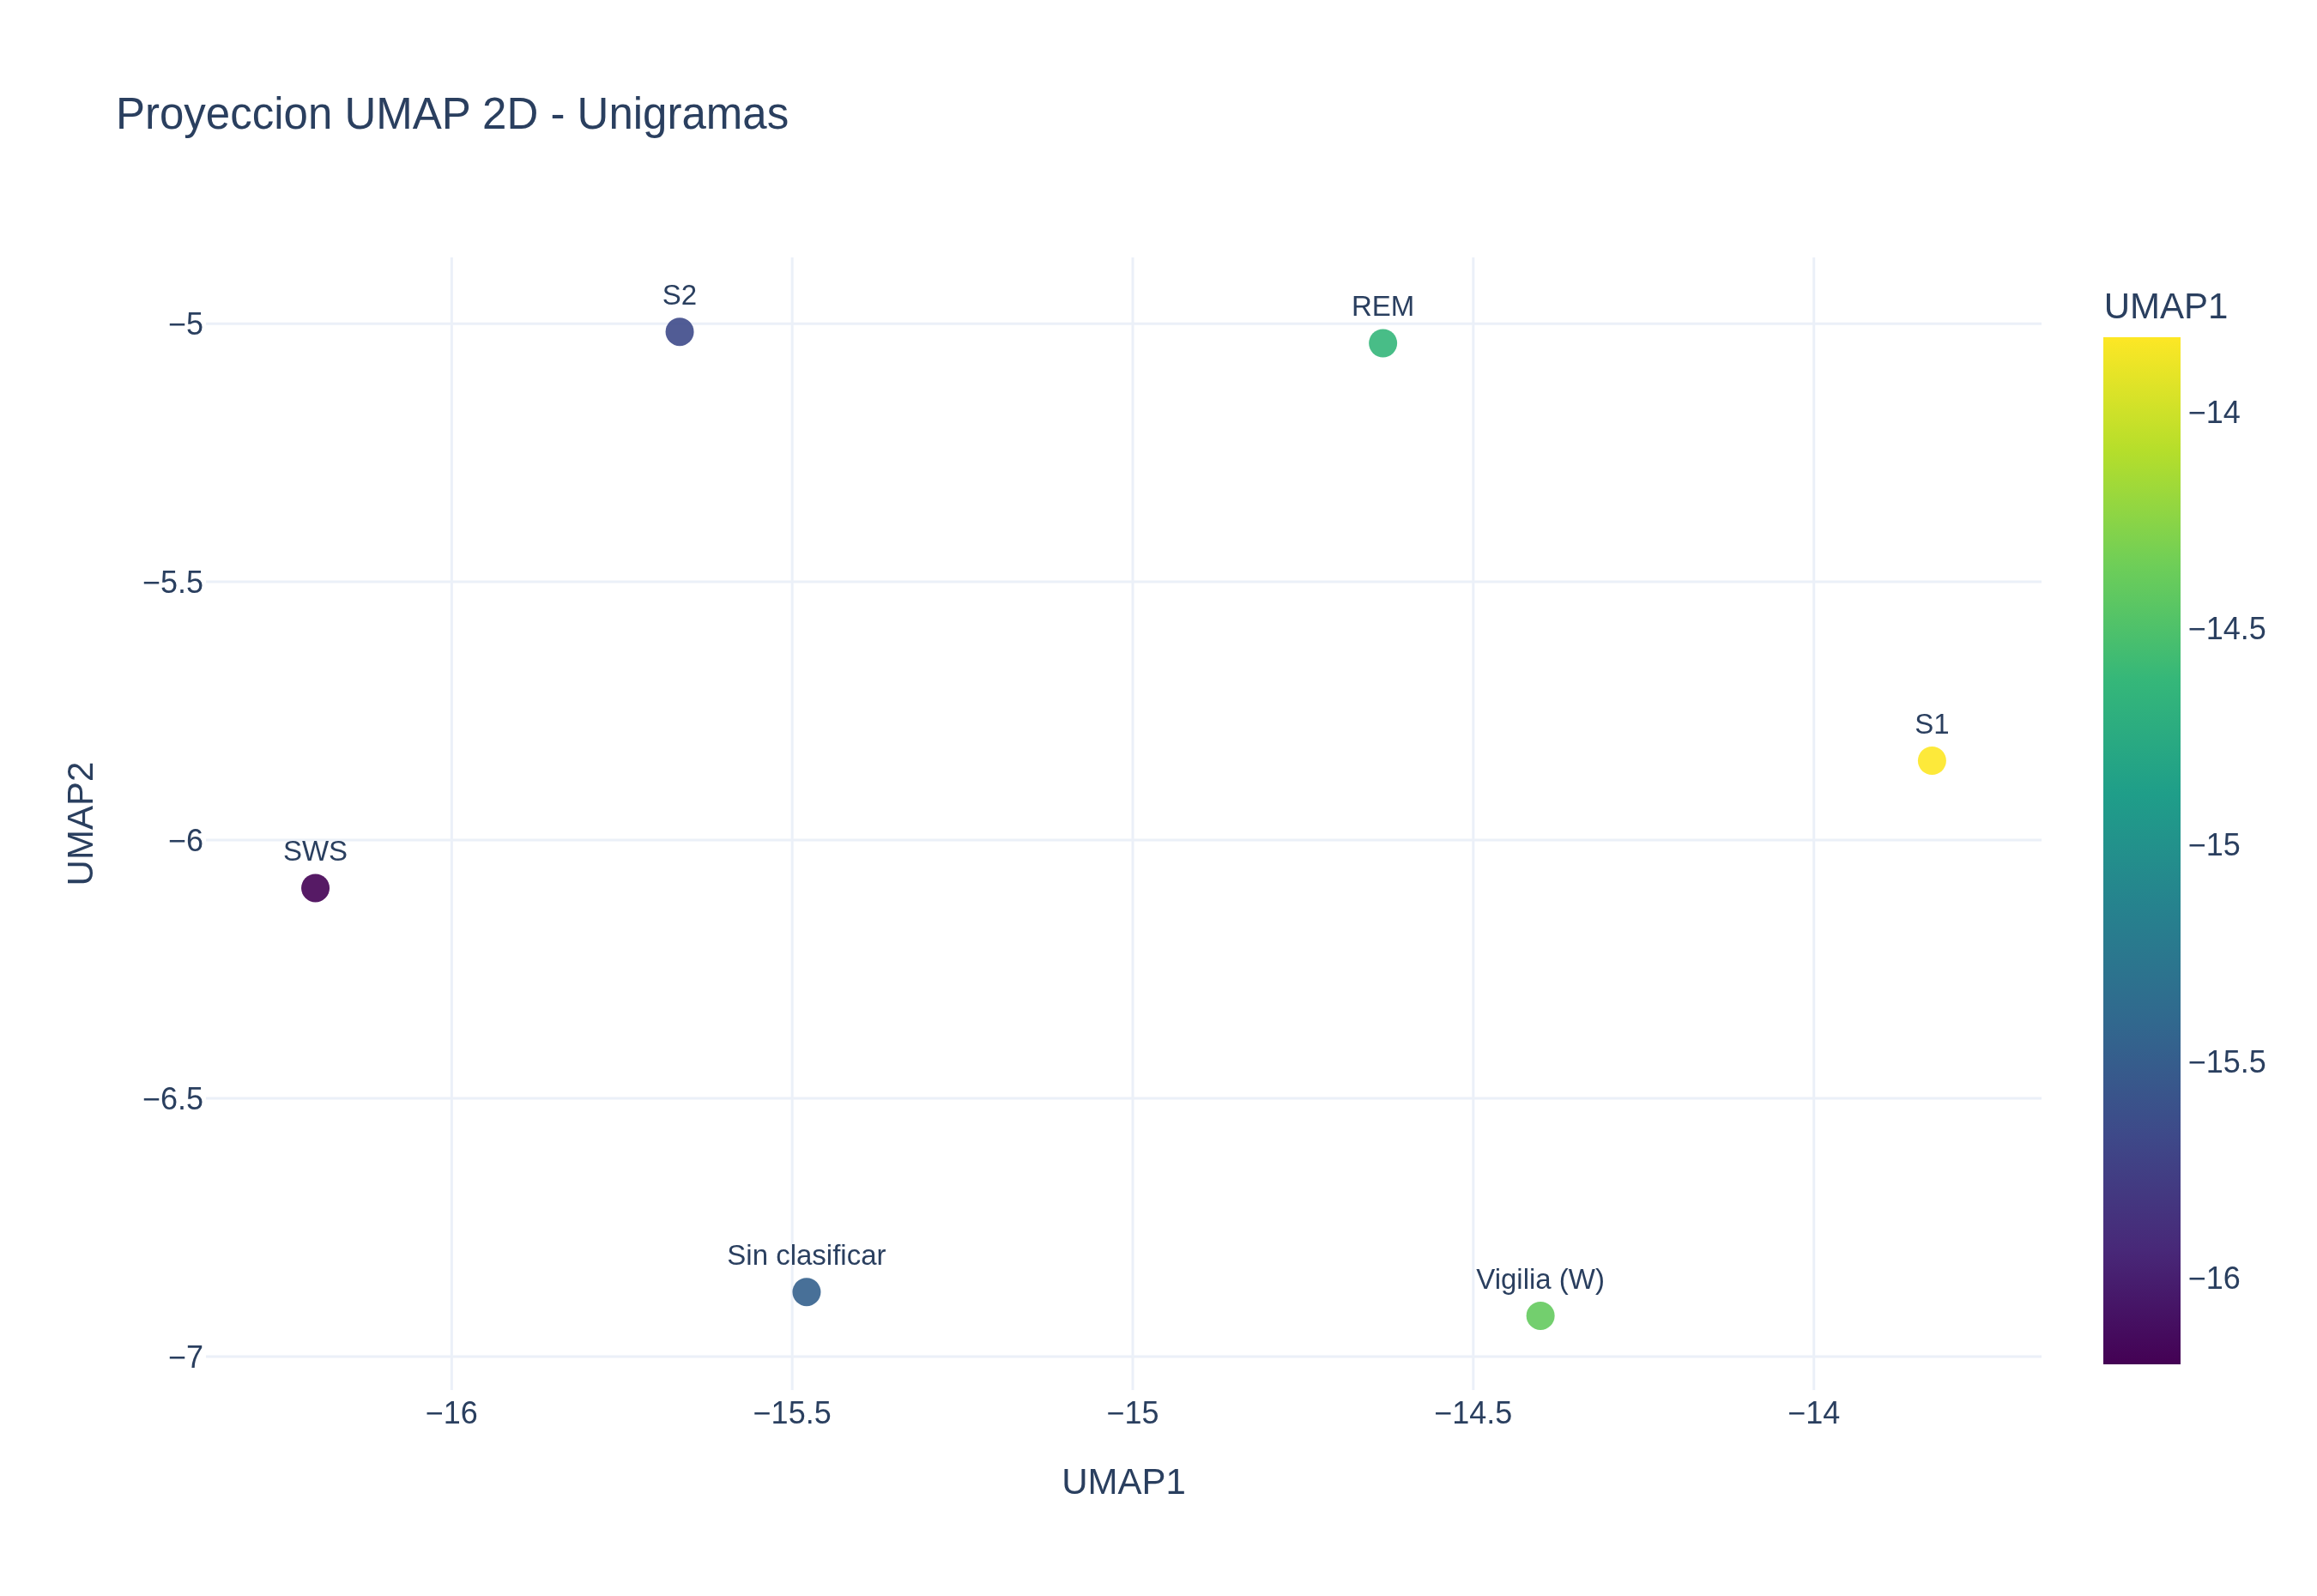
\includegraphics[width=0.95\textwidth]{umap2d_1g.png}
    \caption{Topología basal del espacio latente (Proyección UMAP 2D de Unigramas). Los estados puros revelan la arquitectura fundamental del espacio de fases, con la Fase 2 actuando como nodo central entre el sueño profundo (SWS) y el REM.}
    \label{fig:umap_unigramas_2d}
\end{figure}

\begin{figure}[htbp]
    \centering
    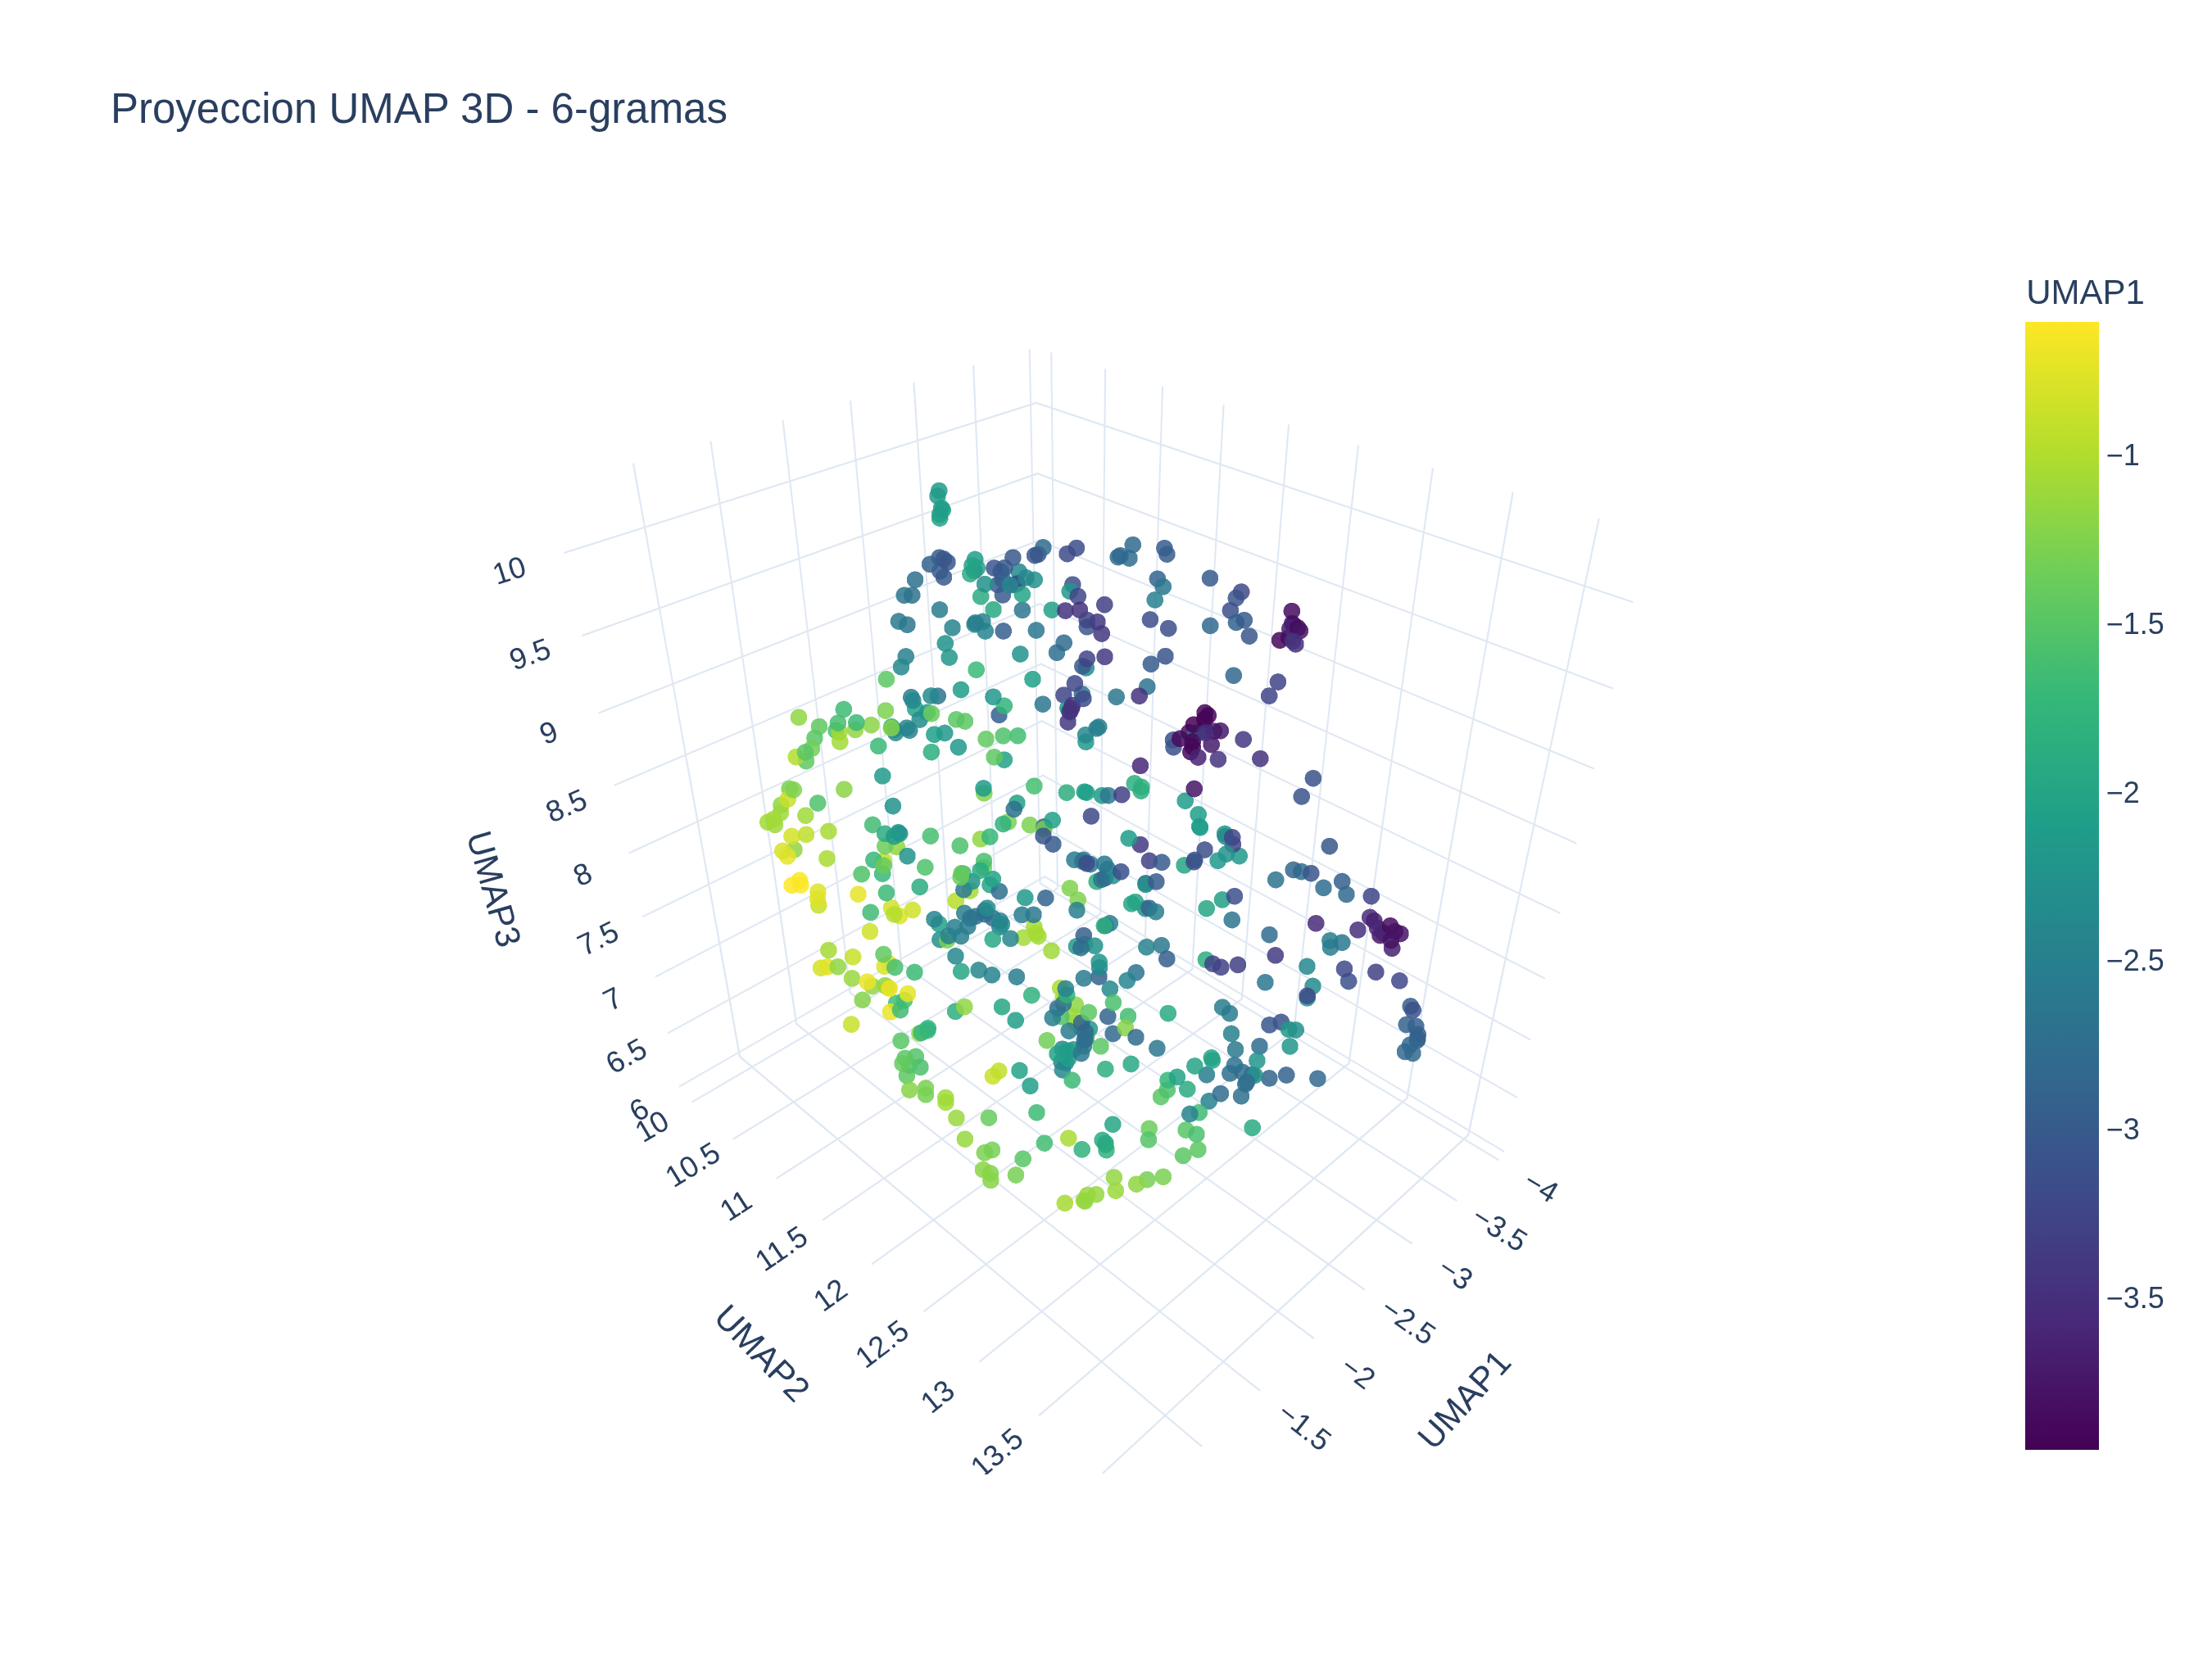
\includegraphics[width=0.95\textwidth]{umap3d_6g.png}
    \caption{Proyección UMAP 3D del espacio de 6-gramas (anticipo). La estructura tridimensional ilustra cómo las secuencias se organizan a lo largo de múltiples ejes de variación fisiológica, formando trayectorias continuas entre los polos de consolidación y activación.}
    \label{fig:umap_6g_3d}
\end{figure}

\subsection{Validación Cuantitativa: Matriz de Similitud Coseno}

Para complementar la visualización topológica con evidencia numérica, calculamos la similitud coseno entre todos los pares de unigramas directamente en el espacio de embeddings de 24 dimensiones del modelo de unigramas (Tabla \ref{tab:similitud_unigramas}). Estos valores son independientes de la proyección UMAP y reflejan las relaciones aprendidas por el modelo.

\begin{table}[htbp]
    \centering
    \caption{Matriz de Similitud Coseno entre Unigramas. Valores positivos indican vectores orientados en direcciones similares; valores negativos indican orientaciones opuestas.}
    \label{tab:similitud_unigramas}
    \begin{tabular}{lrrrrrr}
        \toprule
        & \textbf{W} & \textbf{S1} & \textbf{S2} & \textbf{SWS} & \textbf{REM} & \textbf{S.C.} \\
        \midrule
        \textbf{W} & 1.000 & 0.178 & $-$0.719 & $-$0.221 & $-$0.221 & 0.135 \\
        \textbf{S1} & 0.178 & 1.000 & $-$0.286 & $-$0.593 & 0.040 & $-$0.283 \\
        \textbf{S2} & $-$0.719 & $-$0.286 & 1.000 & 0.302 & $-$0.248 & $-$0.363 \\
        \textbf{SWS} & $-$0.221 & $-$0.593 & 0.302 & 1.000 & $-$0.437 & 0.091 \\
        \textbf{REM} & $-$0.221 & 0.040 & $-$0.248 & $-$0.437 & 1.000 & $-$0.073 \\
        \textbf{S.C.} & 0.135 & $-$0.283 & $-$0.363 & 0.091 & $-$0.073 & 1.000 \\
        \bottomrule
    \end{tabular}
\end{table}

Los valores confirman cuantitativamente las observaciones topológicas:
\begin{itemize}
    \item \textbf{Continuidad NREM:} S2 y SWS son los únicos estados de sueño consolidado con similitud claramente positiva ($+$0.302), confirmando su continuidad funcional dentro del NREM.
    \item \textbf{Oposición Vigilia--S2:} La similitud fuertemente negativa entre W y S2 ($-$0.719) refleja que vigilia y sueño consolidado ocupan direcciones opuestas en el espacio vectorial.
    \item \textbf{Aislamiento del REM:} El REM mantiene similitudes negativas con S2 ($-$0.248) y SWS ($-$0.437), confirmando que ocupa una dirección distintiva, coherente con su naturaleza paradójica.
    \item \textbf{Inestabilidad de S1:} S1 se relaciona positivamente con la vigilia ($+$0.178) y negativamente con el sueño profundo ($-$0.593), consistente con su rol de estado de transición superficial.
\end{itemize}

\subsection{Interpretación Fisiológica de la Geometría}

El mapa revela una organización coherente con la fisiología del sueño, validando que el entrenamiento con n-gramas logró capturar, como efecto emergente, la semántica de los estados individuales:

\begin{enumerate}
    \item \textbf{Polaridad de Profundidad:} La dimensión primaria de variación separa los estados de sueño consolidado (S2, SWS) de la vigilia, que aparecen en oposición directa ($-$0.719). El modelo aprendió el concepto de ``profundidad de sueño'' como factor dominante de organización.

    \item \textbf{Ortogonalidad del REM:} El estado REM se agrupa en una región topológicamente distinta, con similitudes negativas frente al NREM. Esto refleja su naturaleza paradójica: espectralmente activo pero conductualmente profundo.

    \item \textbf{Proximidad S2--SWS:} La Fase 2 y el Sueño Profundo aparecen cercanos ($+$0.302), reflejando su continuidad funcional dentro del sueño NREM y confirmando que S2 es la ``puerta de entrada'' al sueño profundo.
\end{enumerate}

\subsection{S2 como Hub Geométrico}

Un hallazgo particularmente relevante es la posición de la \textbf{Fase 2}. Su ubicación le permite actuar como un \textit{nodo de transición}: es el único estado con vínculo positivo hacia el SWS, mientras mantiene direcciones diferenciadas respecto al REM. Esta geometría es coherente con el rol de S2 como ``Hub Dinámico'' identificado en el análisis markoviano: es el estado desde el cual el sistema puede bifurcarse hacia profundización (SWS) o activación paradójica (REM).

\subsection{Conclusión de la Validación Topológica}

La proyección de unigramas confirma que el modelo Word2Vec ha construido un \textbf{sistema de coordenadas biológicamente válido}. Los ``átomos'' del sueño están correctamente posicionados:
\begin{itemize}
    \item Vigilia: polo opuesto al sueño consolidado.
    \item S2 y SWS: polo de consolidación NREM.
    \item REM: dirección distintiva de activación paradójica.
\end{itemize}

Con esta confianza en la arquitectura basal del espacio latente, podemos proceder en la siguiente sección a analizar cómo las secuencias complejas ($N=6$) ``navegan'' a través de este mapa en tiempo real, revelando la dinámica anticipatoria de las transiciones.

\section{Dinámica de Transiciones: Trayectorias Anticipatorias}

Habiendo validado la topología estática, abordamos la \textbf{Hipótesis H3 (Dinámica)}: la representación vectorial de la salida de S2 codifica información sobre su destino (REM frente a SWS) y permite anticipar la transición antes de que sea clínicamente visible. Esta sección aporta la primera pieza de evidencia ---la \textit{geometría} del espacio de embeddings---, que más adelante se complementa con la prueba predictiva directa del modelo recurrente (Sección \ref{sec:lstm}).

Para ello ejecutamos el experimento de \textbf{Ventanas Deslizantes} (interpolación sintética), midiendo cómo evoluciona la \textbf{Similitud Coseno} de un vector de S2 puro conforme se infiltran progresivamente épocas del estado destino.

\subsection{El Experimento del Deslizador}

Se generaron secuencias sintéticas partiendo de un bloque basal ($t_0$) de 6 épocas de Fase 2. En cada paso temporal $t$, se sustituyó una época de S2 por una del estado destino (REM o SWS), simulando una transición gradual:

\begin{itemize}
    \item \textbf{Origen ($t_0$):} Vector de \texttt{[S2, S2, S2, S2, S2, S2]} $\rightarrow$ Similitud = 1.0
    \item \textbf{Hacia SWS:} Transición progresiva hacia \texttt{[SWS, SWS, SWS, SWS, SWS, SWS]}
    \item \textbf{Hacia REM:} Transición progresiva hacia \texttt{[REM, REM, REM, REM, REM, REM]}
\end{itemize}

Este diseño experimental aísla el efecto puro de cada transición, eliminando la variabilidad de los datos reales.

\subsection{Bifurcación de Trayectorias}

La Figura \ref{fig:trayectorias_bifurcacion} ilustra la evolución de la Similitud Coseno respecto al vector origen ($t_0$), para las dos rutas de destino. La Tabla \ref{tab:deslizador} reporta los valores exactos.

\begin{figure}[htbp]
    \centering
    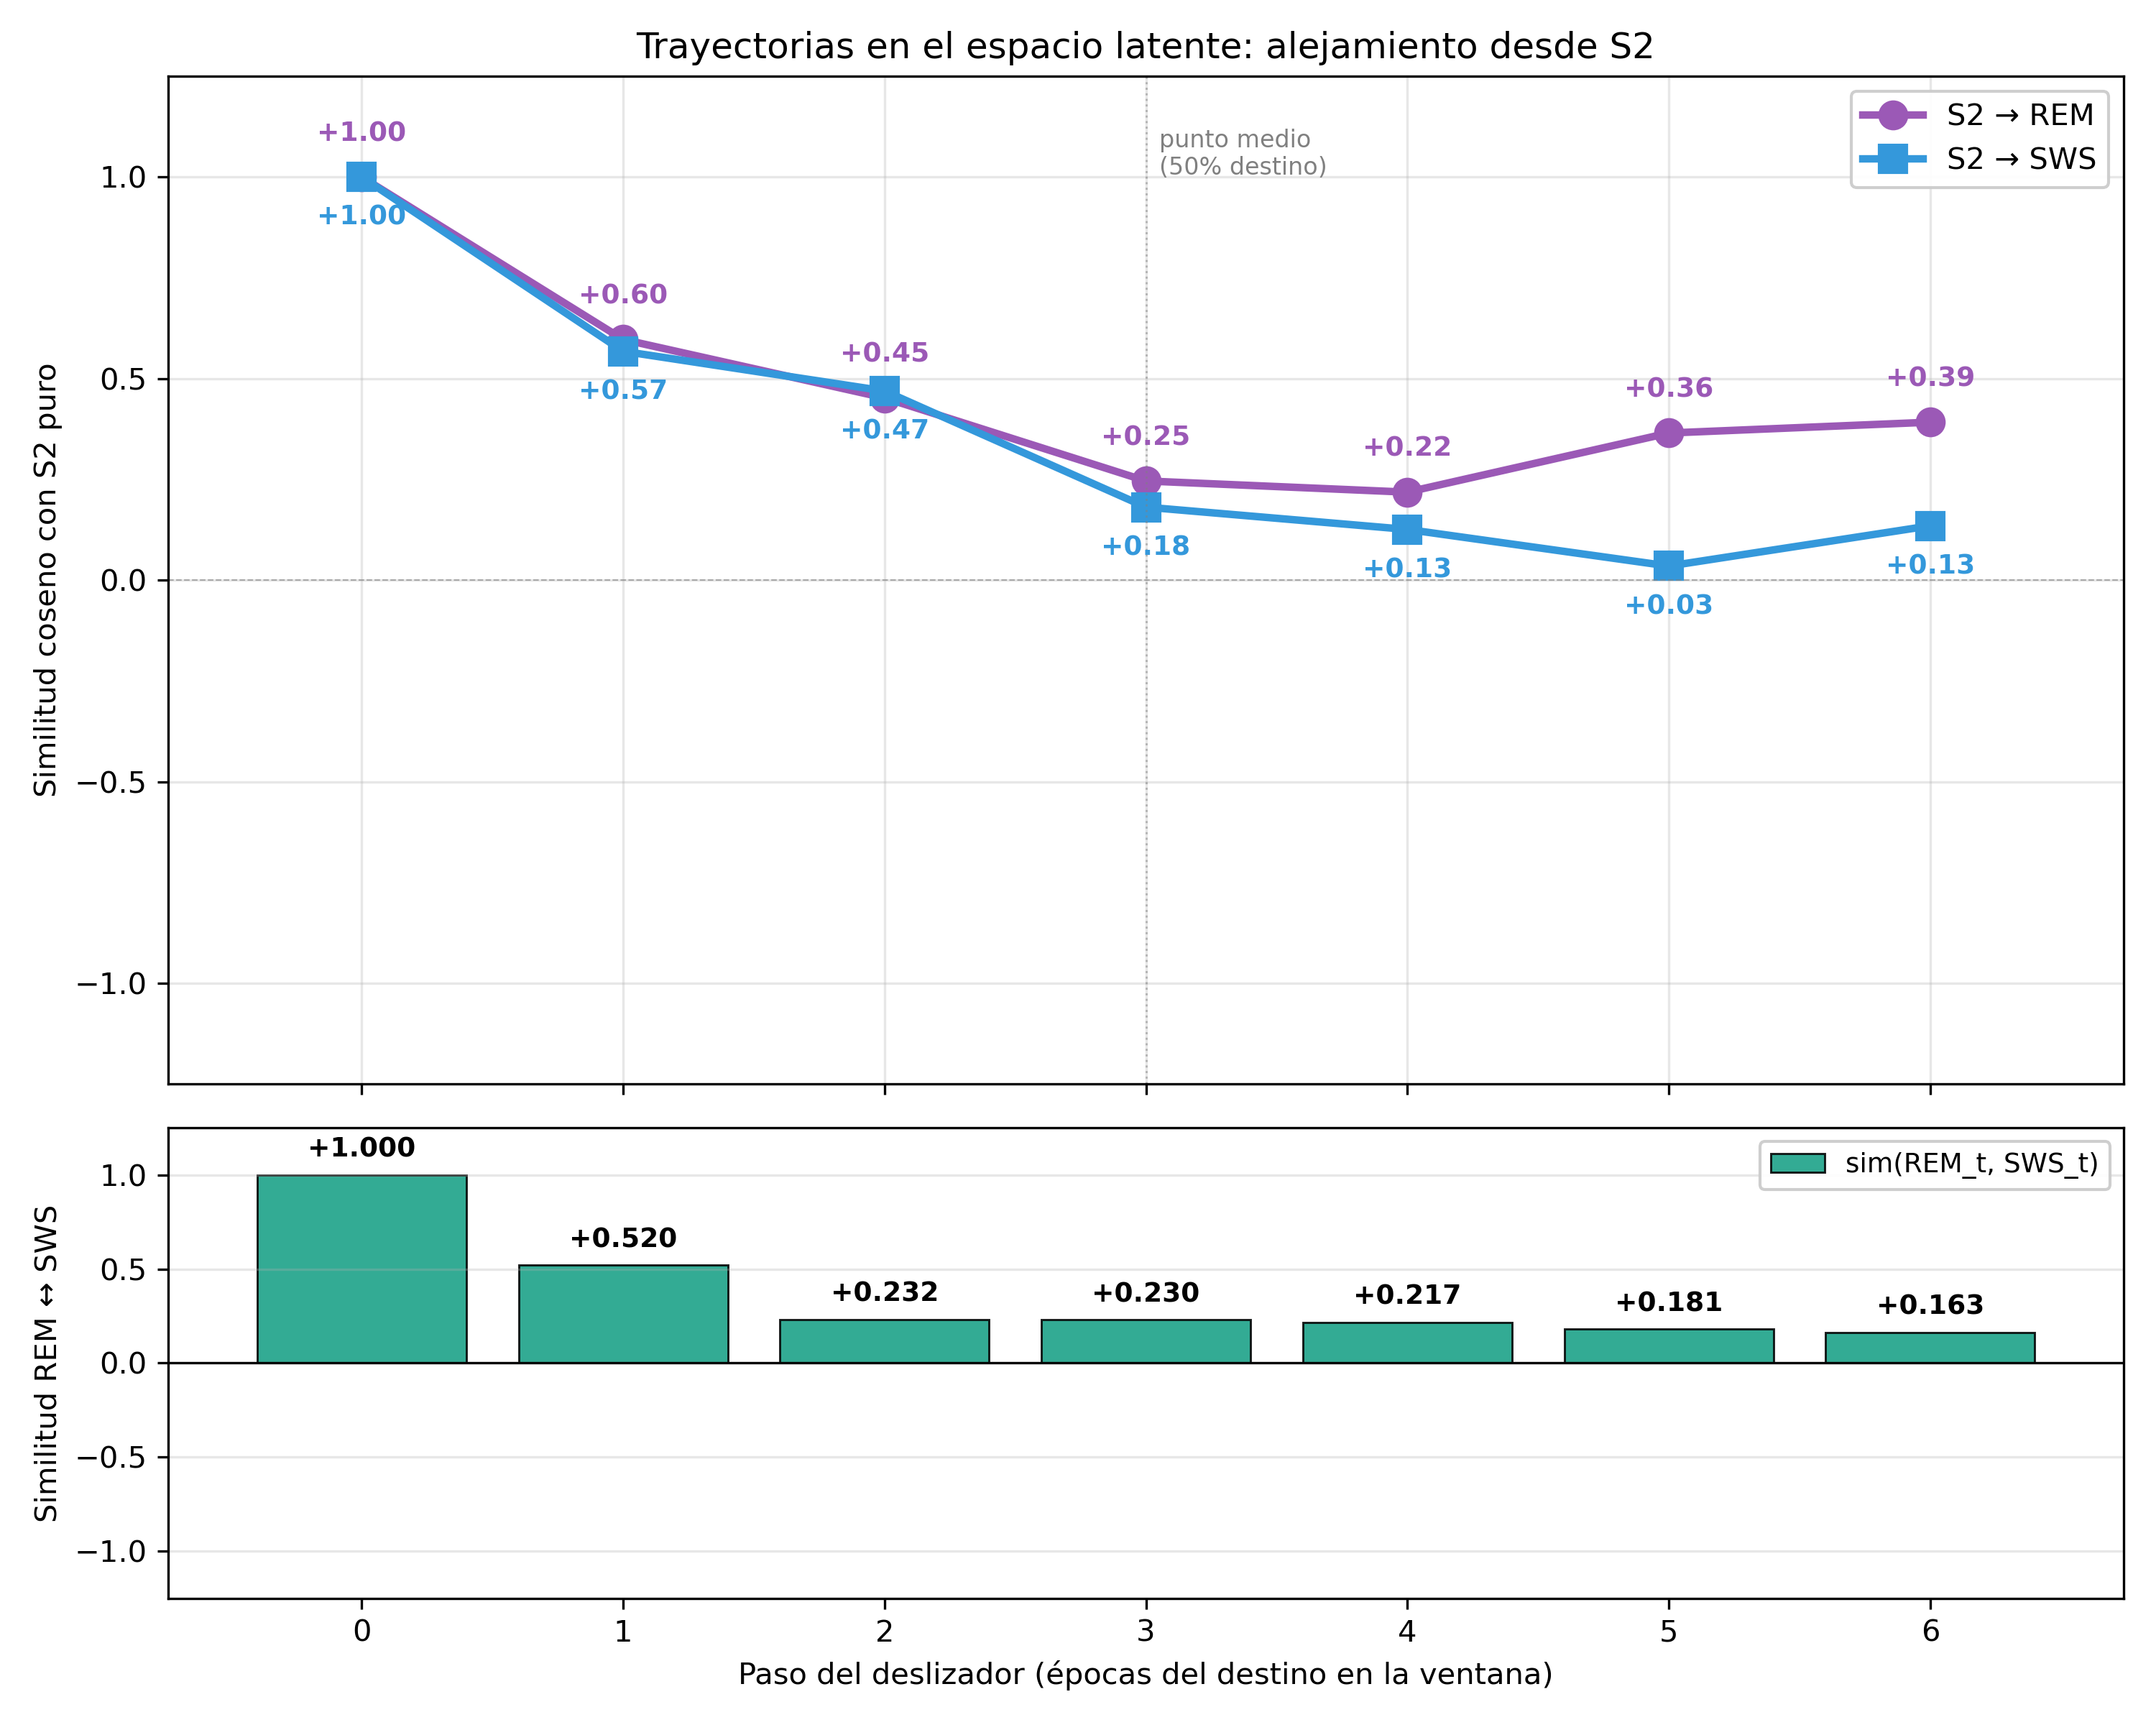
\includegraphics[width=0.95\textwidth]{similitud_origen.png}
    \caption{Dinámica de separación de fases ($N=6$): similitud coseno respecto al origen S2 conforme se infiltran épocas del destino. Las dos rutas (hacia SWS y hacia REM) describen trayectorias distinguibles, evidencia de que la representación de S2 codifica información sobre su destino.}
    \label{fig:trayectorias_bifurcacion}
\end{figure}

\begin{table}[htbp]
\centering
\caption{Similitud coseno respecto al origen S2 en cada paso de infiltración (datos reales).}
\label{tab:deslizador}
\begin{tabular}{ccc}
\hline
\textbf{Paso} & \textbf{Hacia SWS} & \textbf{Hacia REM} \\
\hline
0 & 1.000 & 1.000 \\
1 & 0.568 & 0.597 \\
2 & 0.469 & 0.452 \\
3 & 0.181 & 0.246 \\
4 & 0.126 & 0.218 \\
5 & 0.035 & 0.365 \\
6 & 0.135 & 0.392 \\
\hline
\end{tabular}
\end{table}

\subsubsection{Análisis Cuantitativo de la Divergencia}

Los resultados aportan la primera evidencia geométrica de la \textbf{Hipótesis H3}: la trayectoria del vector depende del destino. Las diferencias clave son:

\begin{enumerate}
    \item \textbf{Hacia SWS (alejamiento profundo):} La ruta hacia el sueño profundo aleja más la representación del origen S2. El área bajo la curva de similitud al origen es de 1.946, y alcanza su valor mínimo en el paso 5 (similitud 0.035), justo antes de consolidarse como bloque SWS puro.

    \item \textbf{Hacia REM (alejamiento moderado con recuperación):} La ruta hacia REM conserva mayor similitud con el origen (área bajo la curva de 2.574) y, tras el descenso intermedio, repunta hacia el final (0.365 en el paso 5 y 0.392 en el paso 6) a medida que el bloque REM se consolida en una dirección propia.

    \item \textbf{Distinguibilidad de rutas:} Las dos trayectorias son separables a lo largo de toda la infiltración, lo que indica que el espacio de embeddings no representa todas las salidas de S2 por igual, sino de forma diferenciada según el destino.
\end{enumerate}

\subsection{Qué Prueba y Qué No Prueba el Deslizador}

Conviene ser preciso sobre el alcance de este experimento. Las secuencias del deslizador son \textbf{sintéticas} y construidas insertando progresivamente el símbolo destino (por ejemplo, \texttt{2-2-2-2-4-4} ya contiene dos épocas de REM). Por tanto, que la ventana ``hacia REM'' se parezca cada vez más a REM no es, por sí mismo, una demostración de anticipación: en parte refleja que el destino ya está presente en el token. Además, existe una \textbf{limitación arquitectónica} de fondo: una época de S2 pura es siempre el mismo token (\texttt{2-2-2-2-2-2}), de modo que Word2Vec le asigna \textit{un único vector} con independencia de hacia dónde transite la noche real; un embedding estático no puede, por construcción, distinguir una ``S2 pre-REM'' de una ``S2 pre-SWS'' mientras la ventana siga siendo S2 pura.

Lo que el deslizador sí establece es que la \textbf{geometría del espacio de embeddings está bien organizada y es coherente con la fisiología}: las rutas de salida hacia SWS y hacia REM ocupan direcciones distintas y separables, con asimetrías reproducibles. Es una validación de la representación, no una prueba de anticipación en datos reales. La evidencia de anticipación \textit{propiamente dicha} ---asignar mayor probabilidad al destino antes de que la transición ocurra en hipnogramas reales--- la aporta el modelo recurrente con memoria (Sección \ref{sec:lstm}), que sí puede dar valores distintos a dos épocas de S2 idénticas según la historia que las precede.

\subsection{Control de Subrogados y Prueba de Permutación}

Como \textbf{control de robustez de la Hipótesis H3}, repetimos el experimento utilizando \textbf{datos subrogados} (\textit{shuffled}): se destruye la secuencia cronológica de las fases del sueño pero se preservan sus frecuencias globales, de modo que cualquier diferencia respecto a los datos reales debe atribuirse al \textit{orden} y no a la composición.

\begin{figure}[htbp]
    \centering
    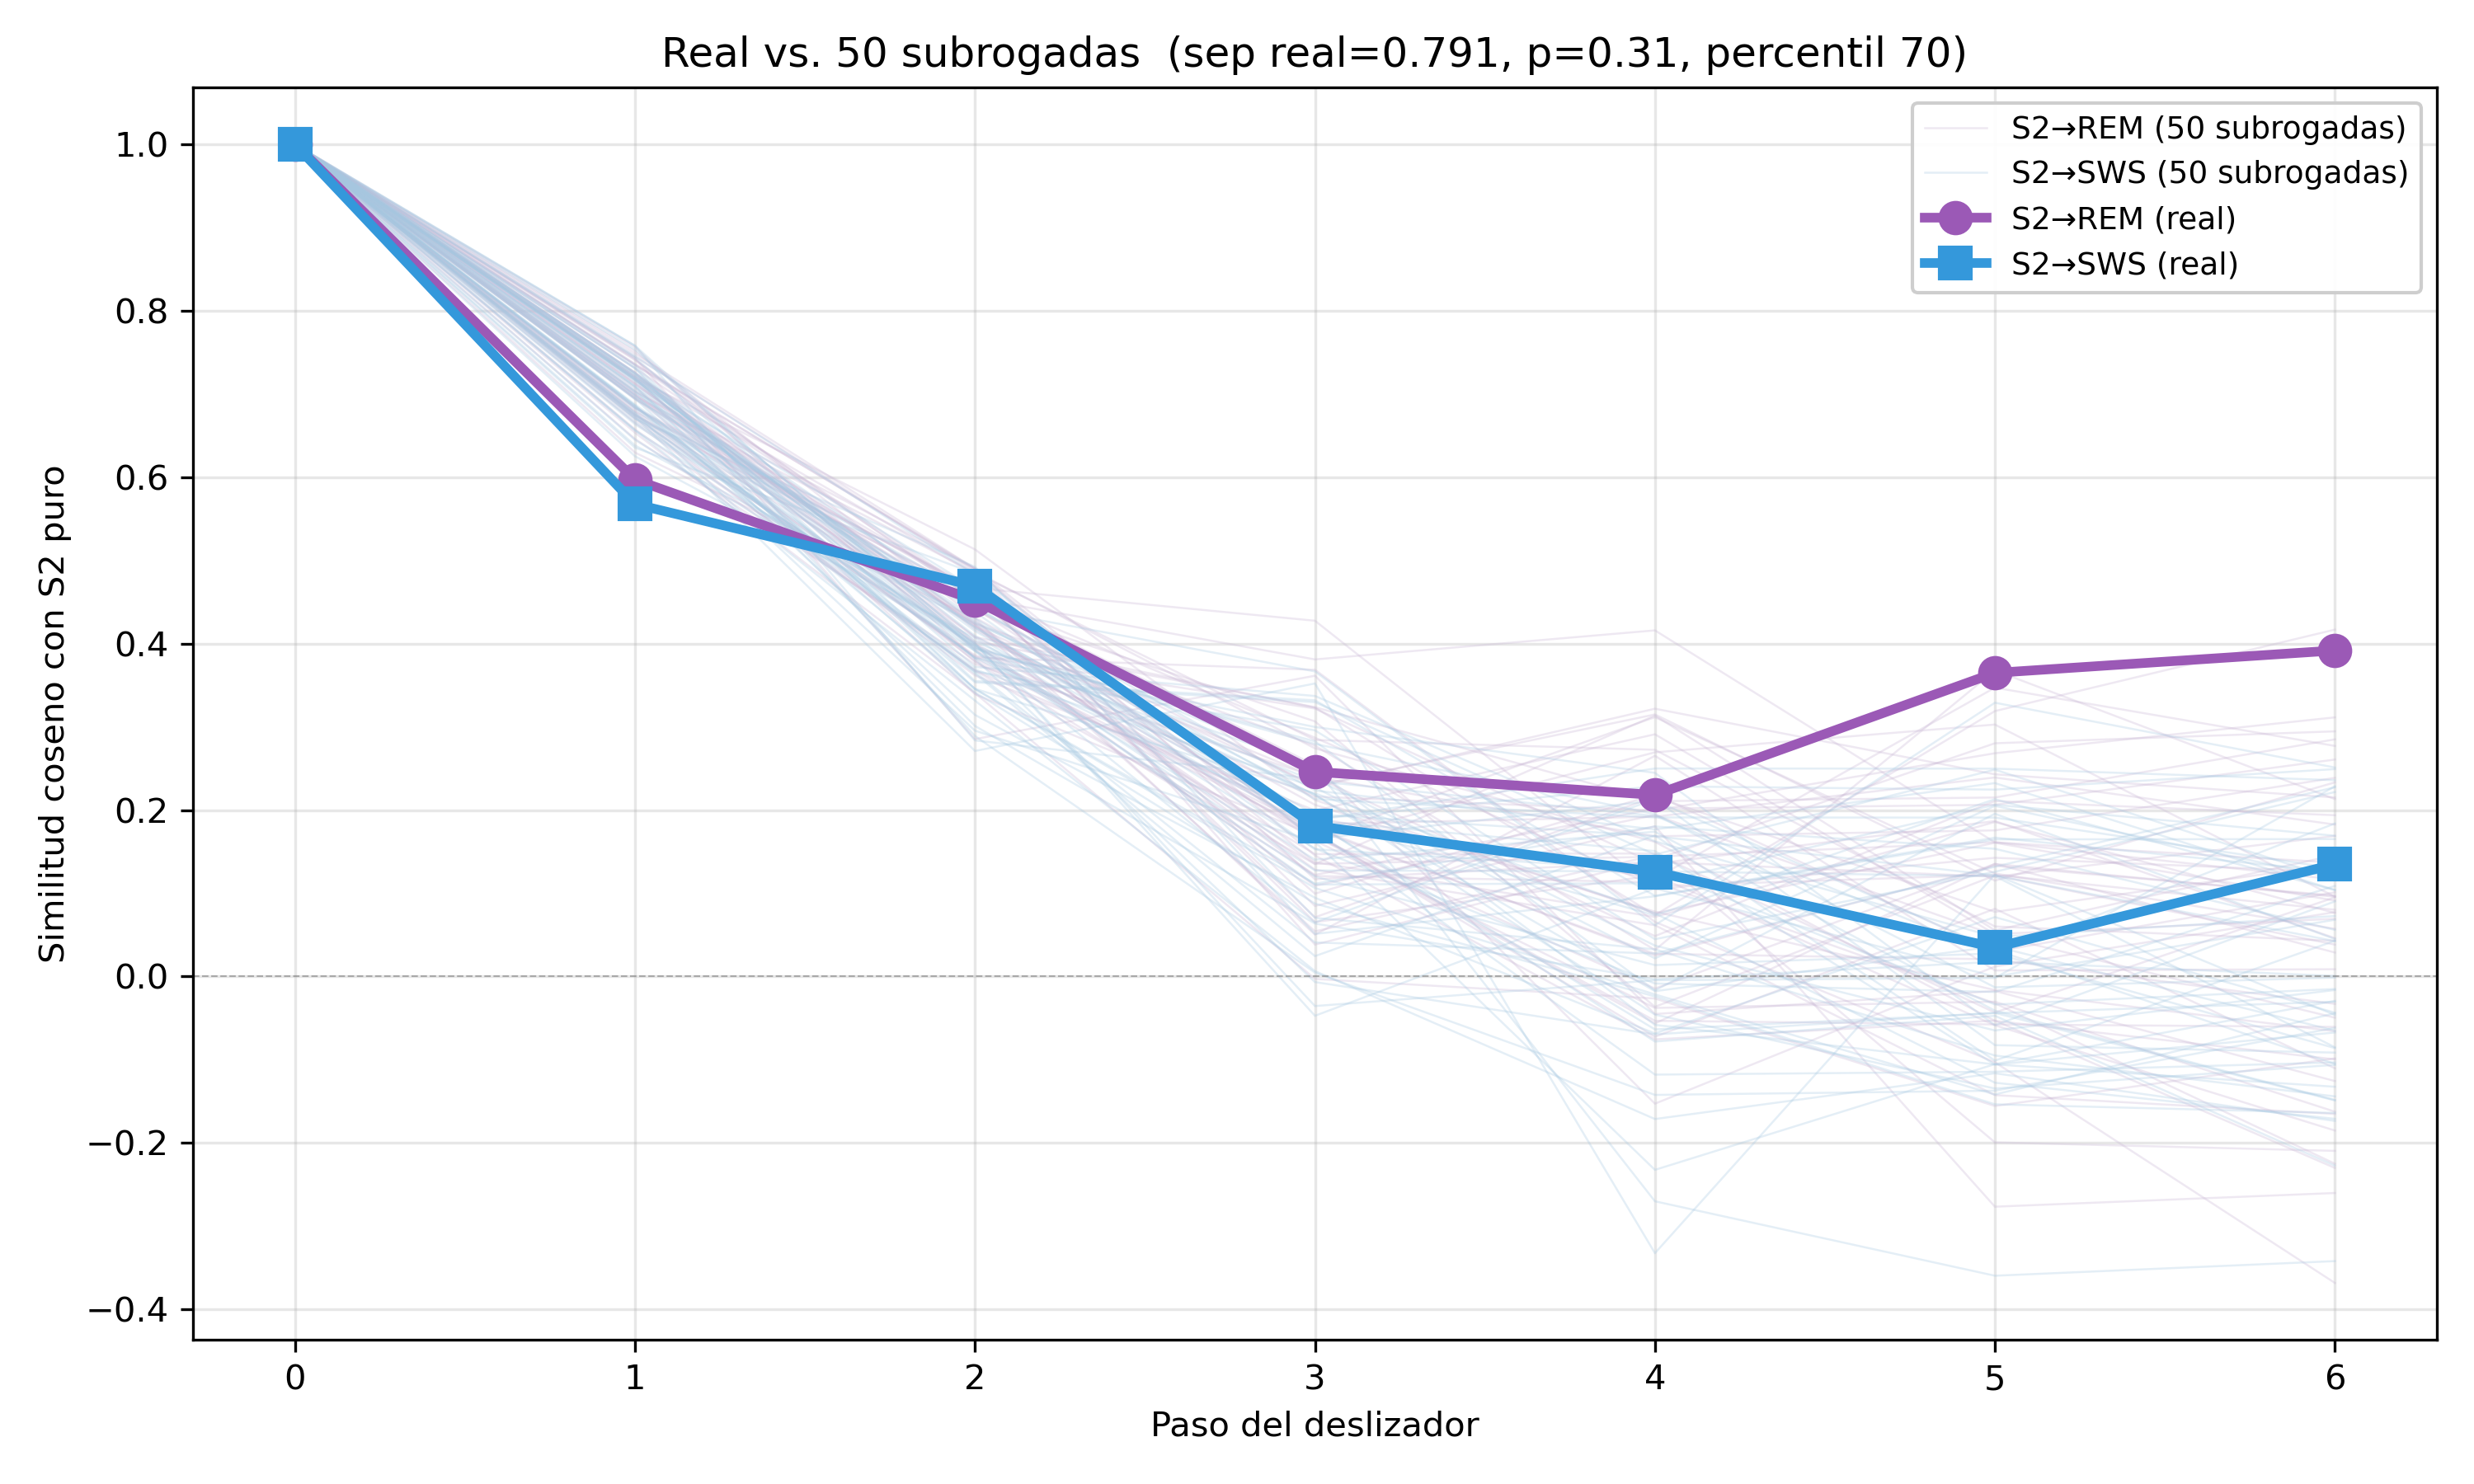
\includegraphics[width=0.95\textwidth]{real_vs_surrogate.png}
    \caption{Comparación de los datos reales frente a las \textbf{50 realizaciones subrogadas} ($N=6$). Las líneas sólidas son las trayectorias reales (S2$\rightarrow$REM y S2$\rightarrow$SWS); las líneas tenues son las 50 trayectorias subrogadas (cada una con su propia permutación intra-paciente y su reentrenamiento independiente de Word2Vec). Las trayectorias reales quedan dentro del haz de las subrogadas: la separación observada no se distingue de la que produce el azar, como confirma la prueba de permutación (Figura \ref{fig:null_dist}).}
    \label{fig:surrogates}
\end{figure}

\subsubsection{Interpretación del Control}

Una \textit{única} realización subrogada produce una separación acumulada de \textbf{0.585} frente a \textbf{0.791} en los datos reales ---una razón de 1.351---, lo que a primera vista sugeriría que el orden temporal aporta la diferencia. Sin embargo, \textbf{una sola permutación no constituye una prueba de significancia}: el valor subrogado depende de la realización concreta.

\textbf{Prueba de permutación.} Para evaluarlo correctamente generamos una \textbf{distribución nula} con \textbf{50 realizaciones subrogadas} independientes (cada una con su propia permutación intra-paciente y su reentrenamiento completo de Word2Vec). El resultado refuta el control de una sola realización: la separación real (0.791) cae en el \textbf{percentil 70} de la distribución nula ---\textbf{15 de 50} subrogados separan \textit{más} que los datos reales---, con un \textbf{$p$-valor empírico de 0.31} (Figura \ref{fig:null_dist}). La separación de trayectorias del deslizador \textbf{no es estadísticamente distinguible de la que produce el azar}.

\begin{figure}[htbp]
    \centering
    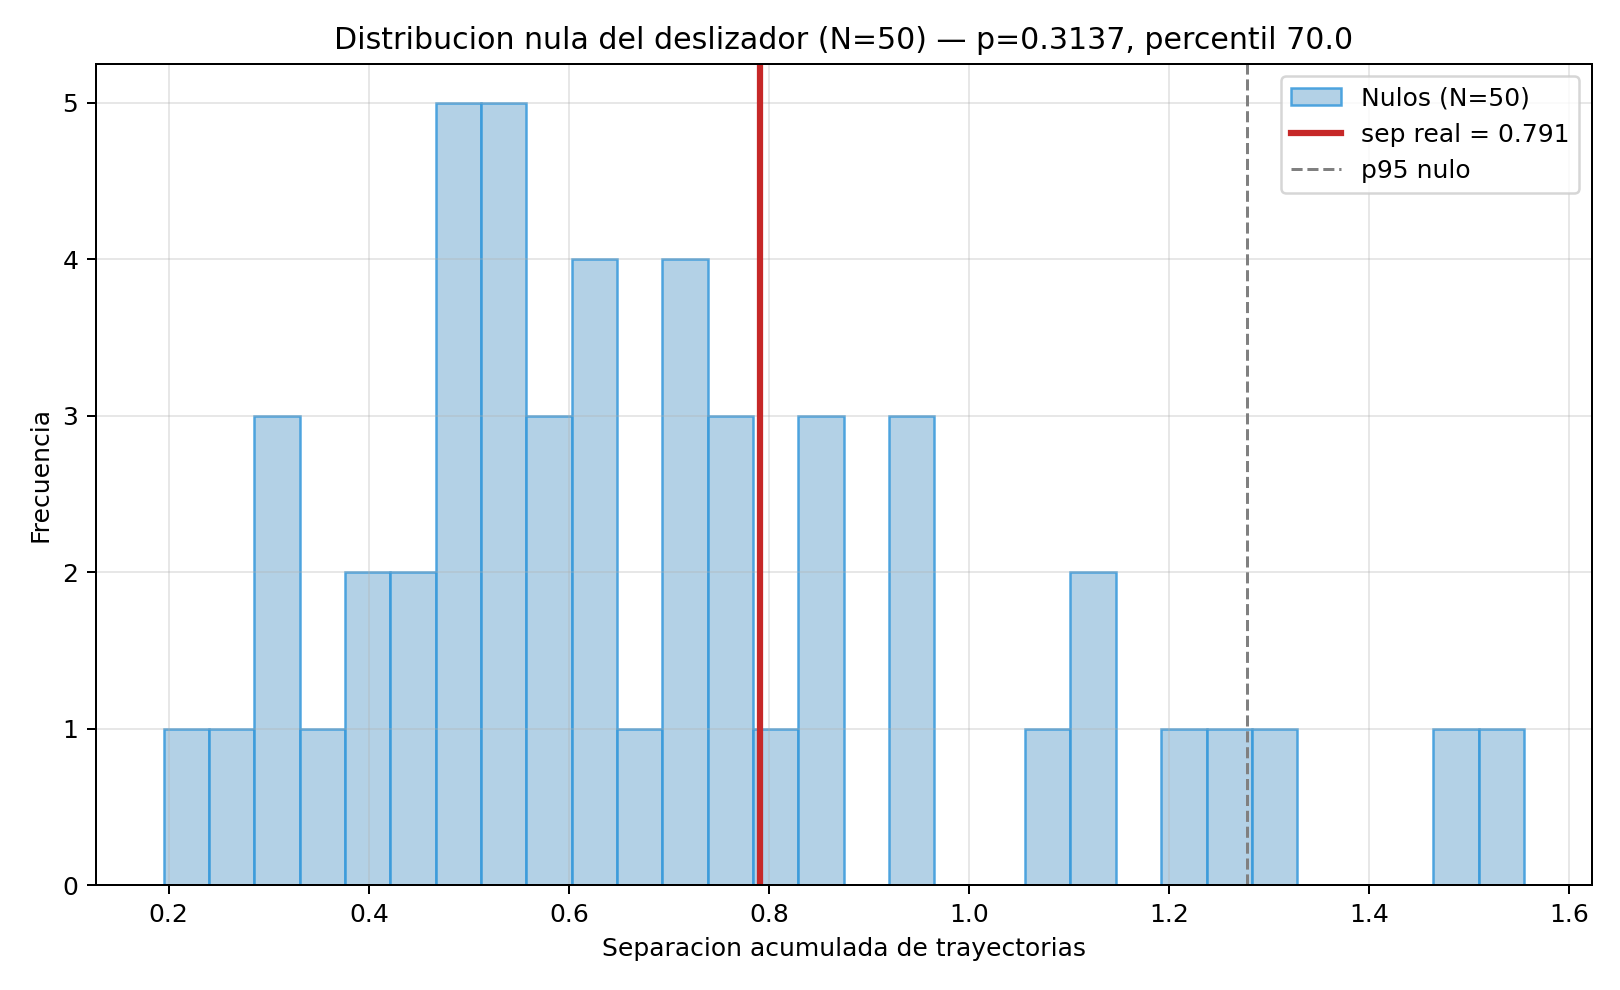
\includegraphics[width=0.9\textwidth]{null_distribution.png}
    \caption{Distribución nula de la separación de trayectorias (50 subrogados con reentrenamiento independiente de Word2Vec). La separación real (línea roja, 0.791) queda en el percentil 70 ($p=0.31$); la razón 1.351 de una única realización era una extracción atípicamente baja del nulo.}
    \label{fig:null_dist}
\end{figure}

\textbf{Por qué falla el control.} Al permutar las fases dentro de cada noche se destruye la inercia del sueño y el vocabulario de 6-gramas se dispara (de 2817 a unos 16\,000 tokens distintos); los \textit{embeddings} de las trayectorias sintéticas pasan a estimarse sobre ese vocabulario ruidoso y adquieren una varianza alta, de modo que los subrogados producen con frecuencia separaciones \textit{mayores} que los datos reales por puro azar. Este resultado, junto con el colapso ante ventanas disjuntas (Sección \ref{sec:deslizador_stride}), confirma que la geometría del deslizador es una \textbf{ilustración del espacio latente y no una prueba de anticipación}. La evidencia propiamente dicha de H3 ---anticipación sobre datos reales--- descansa en la red \textbf{LSTM} (Sección \ref{sec:lstm}), que sí supera su propio control con secuencias barajadas.

\subsection{Control de Robustez: Ventanas Disjuntas}
\label{sec:deslizador_stride}

El deslizador se construyó sobre ventanas \textbf{solapadas} (paso 1): dos 6-gramas consecutivos comparten cinco de sus seis épocas, lo que introduce autocorrelación entre tokens vecinos (limitación ya señalada en la metodología). Para evaluar cuánto de la separación de trayectorias depende de ese solapamiento, reentrenamos Word2Vec con \textbf{ventanas disjuntas} (paso 6, sin solapamiento) y con un paso intermedio (paso 3), y reconstruimos las trayectorias.

\begin{table}[htbp]
\centering
\caption{Robustez del deslizador al paso de tokenización. La separación real cae de forma monótona al reducir el solapamiento y, con ventanas disjuntas, invierte incluso el control de subrogado (razón $<1$). La cobertura de los 13 tokens del deslizador se mantiene completa, de modo que el colapso \textit{no} se debe a tokens ausentes del vocabulario.}
\label{tab:stride}
\footnotesize\setlength{\tabcolsep}{4pt}%
\begin{tabular}{@{}cccccc@{}}
\toprule
\textbf{Paso} & \textbf{Tokens} & \textbf{Cobertura} & \textbf{Sep.\ real} & \textbf{Sep.\ subr.} & \textbf{Razón} \\
\midrule
1 (solapado) & 112\,k & 13/13 & 0.791 & 0.585 & 1.351 \\
3 (intermedio) & 37\,k & 13/13 & 0.611 & 1.262 & 0.484 \\
6 (disjunto) & 18\,k & 13/13 & 0.234 & 0.961 & 0.243 \\
\bottomrule
\end{tabular}
\end{table}

La separación real decrece de forma \textbf{monótona} con el paso (0.791 $\rightarrow$ 0.611 $\rightarrow$ 0.234) y, con ventanas disjuntas, las rutas hacia REM y hacia SWS se vuelven prácticamente indistinguibles (Figura \ref{fig:stride6}): el deslizador deja de bifurcar e incluso falla su propio control de subrogado (razón 0.243, es decir, la separación real resulta \textit{menor} que la subrogada).

\begin{figure}[htbp]
    \centering
    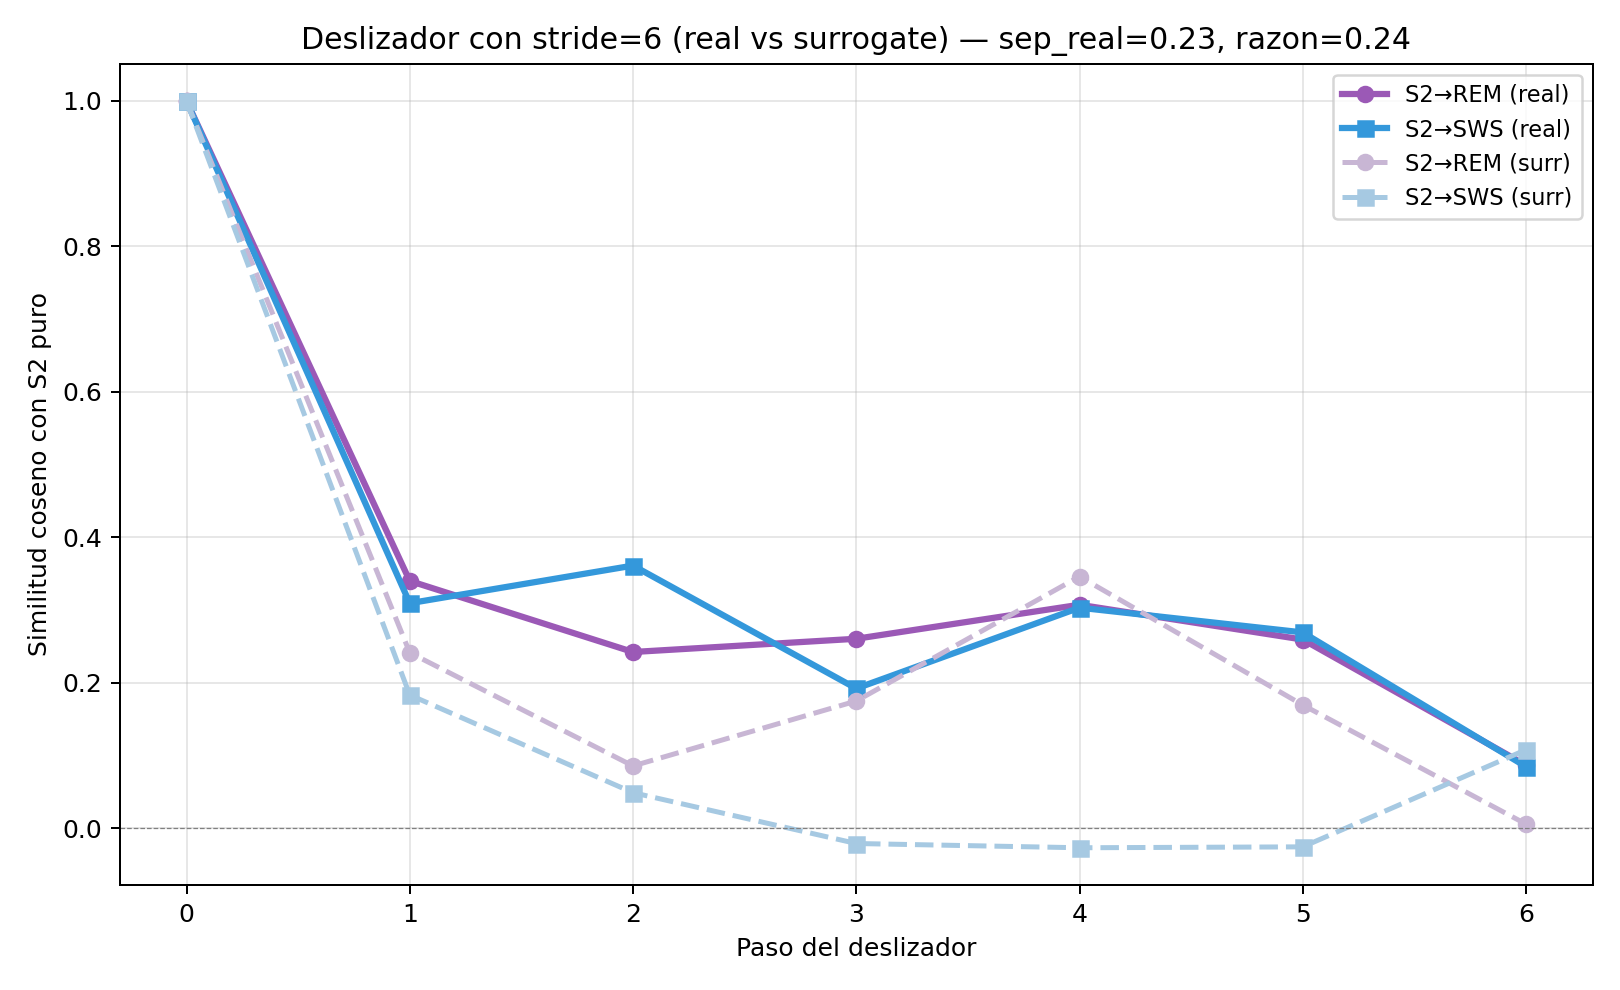
\includegraphics[width=0.9\textwidth]{stride6_real_vs_surrogate.png}
    \caption{Deslizador reentrenado con ventanas disjuntas (paso 6). Las trayectorias reales hacia REM (morado) y hacia SWS (azul) quedan superpuestas: sin solapamiento de ventanas, el espacio de \textit{embeddings} ya no separa el destino.}
    \label{fig:stride6}
\end{figure}

\textbf{Lectura calibrada.} Este colapso es \textbf{consistente con} la preocupación de autocorrelación señalada en la metodología: buena parte del gradiente suave del deslizador lo crea el solapamiento de ventanas. No conviene, sin embargo, sobre-atribuirlo a un único factor: el paso disjunto elimina la autocorrelación \textit{pero también} reduce el corpus en un factor de seis (112\,k $\rightarrow$ 18\,k tokens), lo que por sí solo añade ruido a los \textit{embeddings}; con estos datos ambas causas no se separan limpiamente. Lo que sí queda establecido es que la geometría del deslizador \textbf{no es robusta a la tokenización}, lo que confirma su carácter \textit{ilustrativo} ---de la organización del espacio latente--- y no probatorio. La evidencia central de la Hipótesis H3 \textbf{no se ve afectada}: descansa en la red \textbf{LSTM} (Sección \ref{sec:lstm}), un modelo recurrente por época con memoria genuina, independiente de la geometría de ventanas solapadas de Word2Vec.

\subsection{Síntesis: Confirmación de Hipótesis}

La integración de los experimentos de trayectorias permite concluir:

\begin{table}[htbp]
    \centering
    \caption{Resumen de Validación de Hipótesis}
    \label{tab:resumen_hipotesis}
    \small
    \setlength{\tabcolsep}{4pt}
    \renewcommand{\arraystretch}{1.3}
    \begin{tabular}{@{}>{\raggedright\arraybackslash}p{0.13\textwidth}>{\raggedright\arraybackslash}p{0.26\textwidth}>{\raggedright\arraybackslash}p{0.14\textwidth}>{\raggedright\arraybackslash}p{0.37\textwidth}@{}}
        \toprule
        \textbf{Hipótesis} & \textbf{Predicción} & \textbf{Resultado} & \textbf{Evidencia} \\
        \midrule
        H1 (Estructural) & Sueño no aleatorio, estructurado & Apoyada & Markov: inercia alta, sin atajo SWS$\rightarrow$REM, degradación por ciclos \\
        H2 (Lingüística) & Distribución tipo lenguaje a una escala $N$ & Apoyada & Zipf compatible; $N=6$ por criterio multi-objetivo \\
        H3 (Dinámica) & Salida de S2 dependiente del destino y anticipable & Apoyada (parcial) & LSTM anticipa en datos reales: la pendiente hacia REM es significativa frente a 50 barajadas ($p=0.02$; SWS marginal, $p=0.10$). El deslizador es ilustrativo: su separación no es significativa ($p=0.31$) ni sobrevive a ventanas disjuntas \\
        \bottomrule
    \end{tabular}
\end{table}

\textbf{Interpretación fisiológica:} El espacio vectorial aprendido representa de forma diferenciada las salidas de S2 según su destino. La transición hacia SWS aleja más la ventana del origen S2 (menor similitud acumulada al origen), mientras que la transición hacia REM conserva más rasgos del estado de partida a lo largo de la ventana (mayor similitud acumulada al origen). Esta asimetría es consistente con la arquitectura neurofisiológica subyacente y podría reflejarla, pese a que el modelo no recibió información explícita sobre electrofisiología.

\section{Modelado Predictivo: Red LSTM como Modelo de Lenguaje}
\label{sec:lstm}

Los experimentos anteriores caracterizan la \textit{geometría} del espacio de fases, pero no prueban anticipación sobre datos reales. Esta sección aporta la \textbf{prueba central de la Hipótesis H3}: para evaluar si la secuencia contiene información \textbf{predictiva} de la siguiente fase ---y, en particular, si el modelo anticipa la transición \textit{antes} de que ocurra en hipnogramas reales---, entrenamos una red \textbf{LSTM} sobre los embeddings congelados de los 6-gramas (Capítulo \ref{marcoteo}), tratando la noche de sueño como un modelo de lenguaje que estima $P(w_t \mid w_{<t})$. A diferencia del deslizador, la memoria recurrente permite que dos épocas de S2 idénticas reciban probabilidades distintas según la historia que las precede, condición necesaria para hablar de anticipación.

\subsection{Desempeño Global frente a Líneas Base}

La Tabla \ref{tab:lstm_resumen} compara la LSTM con dos líneas base: un modelo de Markov de primer orden y un predictor de persistencia (``la siguiente fase es igual a la actual''). La Figura \ref{fig:lstm_vs_markov} ilustra la comparación.

\textbf{¿Cómo se leen estas métricas?} La \textbf{exactitud} es simplemente el porcentaje de épocas predichas correctamente; al estar el sueño dominado por unas pocas fases muy frecuentes (sobre todo S2), puede ser engañosamente alta. El \textbf{Macro-F1} corrige ese sesgo: el F1 combina en un solo número la precisión y la cobertura de cada fase (su media armónica), y el prefijo ``macro'' indica que se promedian los F1 de las cinco fases dando a cada una el mismo peso, de modo que acertar una fase rara cuenta tanto como acertar una frecuente. Las dos últimas columnas repiten ambas ideas pero \textbf{solo sobre los instantes de cambio de fase} (las transiciones), que son los momentos clínicamente interesantes y los más difíciles de predecir.

\begin{table}[htbp]
\centering
\caption{Desempeño de la LSTM frente a líneas base. La columna ``transición'' mide la exactitud restringida a los instantes en que la fase realmente cambia.}
\label{tab:lstm_resumen}
\noindent\adjustbox{max width=\textwidth}{%
\begin{tabular}{lrrrr}
\hline
\textbf{Modelo} & \textbf{Exactitud} & \textbf{Macro-F1} & \textbf{Exact. transición} & \textbf{F1 transición} \\
\hline
Markov (1.\textsuperscript{er} orden) & 0.880 & 0.823 & 0.000 & 0.000 \\
Persistencia & 0.880 & 0.823 & 0.000 & 0.000 \\
LSTM (real) & 0.744 & 0.608 & 0.288 & 0.238 \\
LSTM (subrogada) & 0.262 & 0.213 & --- & --- \\
\hline
\end{tabular}}
\end{table}

\begin{figure}[htbp]
    \centering
    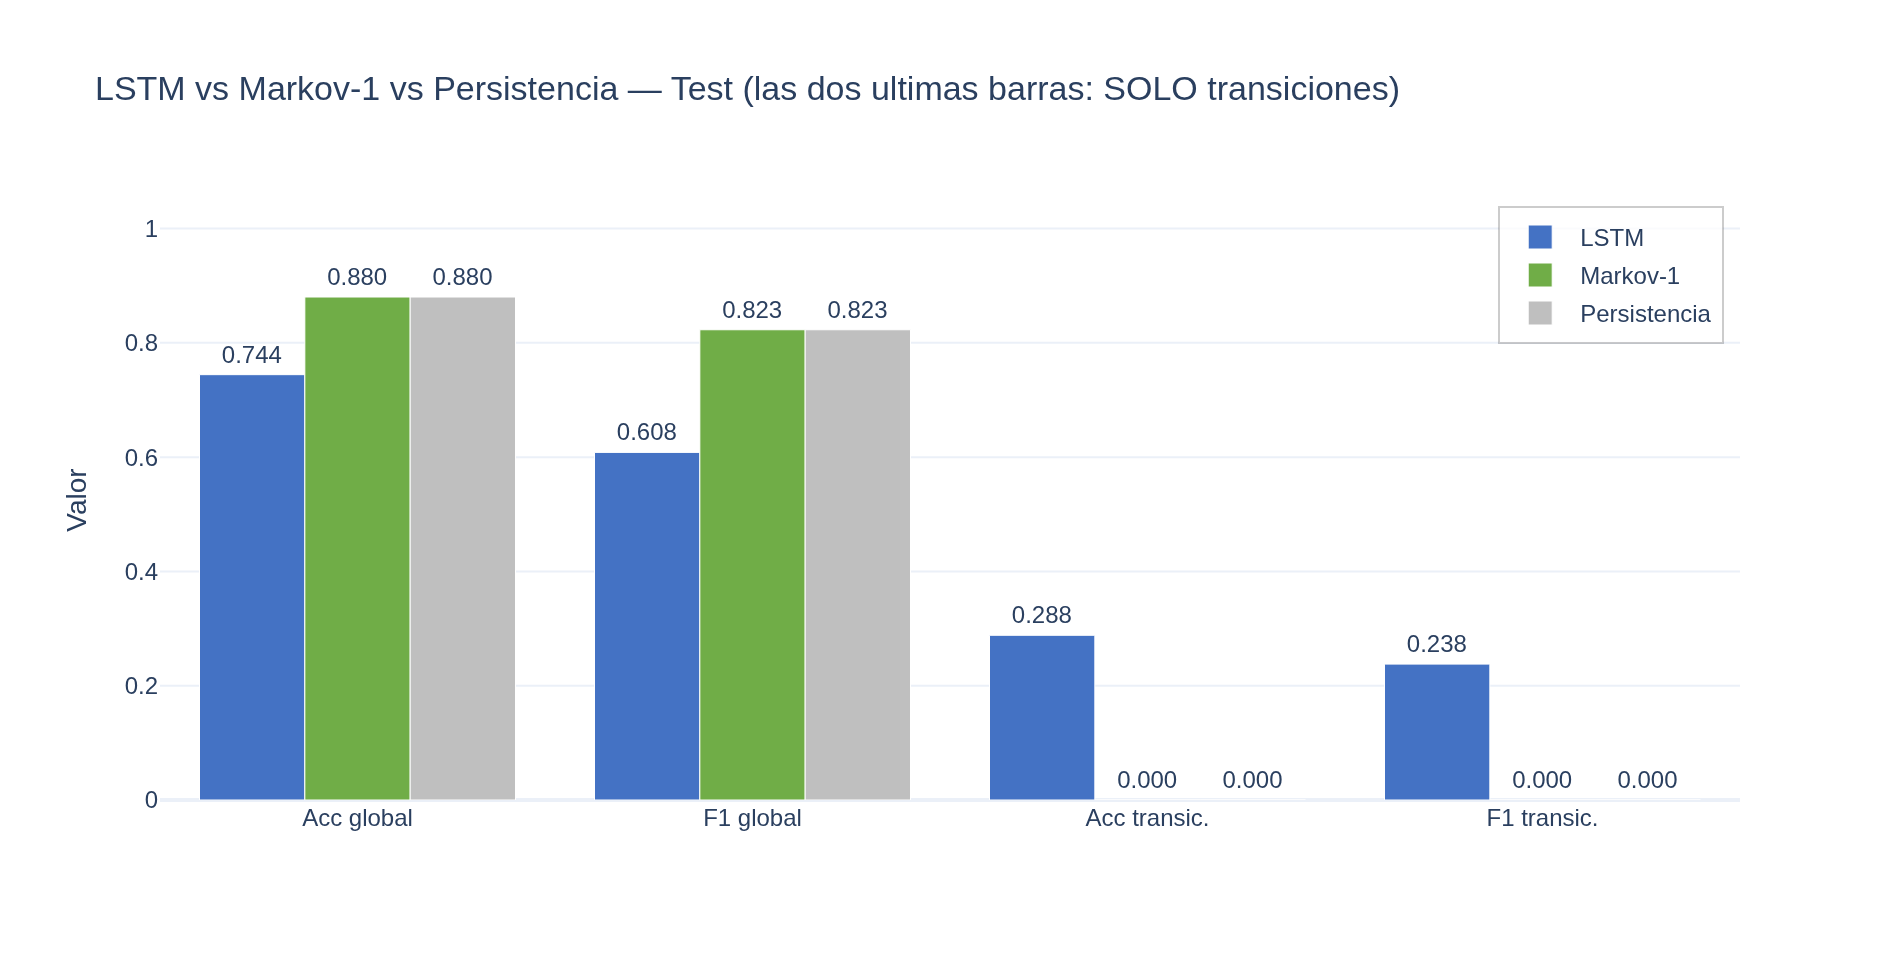
\includegraphics[width=0.95\textwidth]{lstm_vs_markov.png}
    \caption{Comparación de la LSTM frente a los modelos de Markov y de persistencia. La matriz de confusión correspondiente a la LSTM se muestra en la Figura \ref{fig:confusion_lstm}.}
    \label{fig:lstm_vs_markov}
\end{figure}

\begin{figure}[htbp]
    \centering
    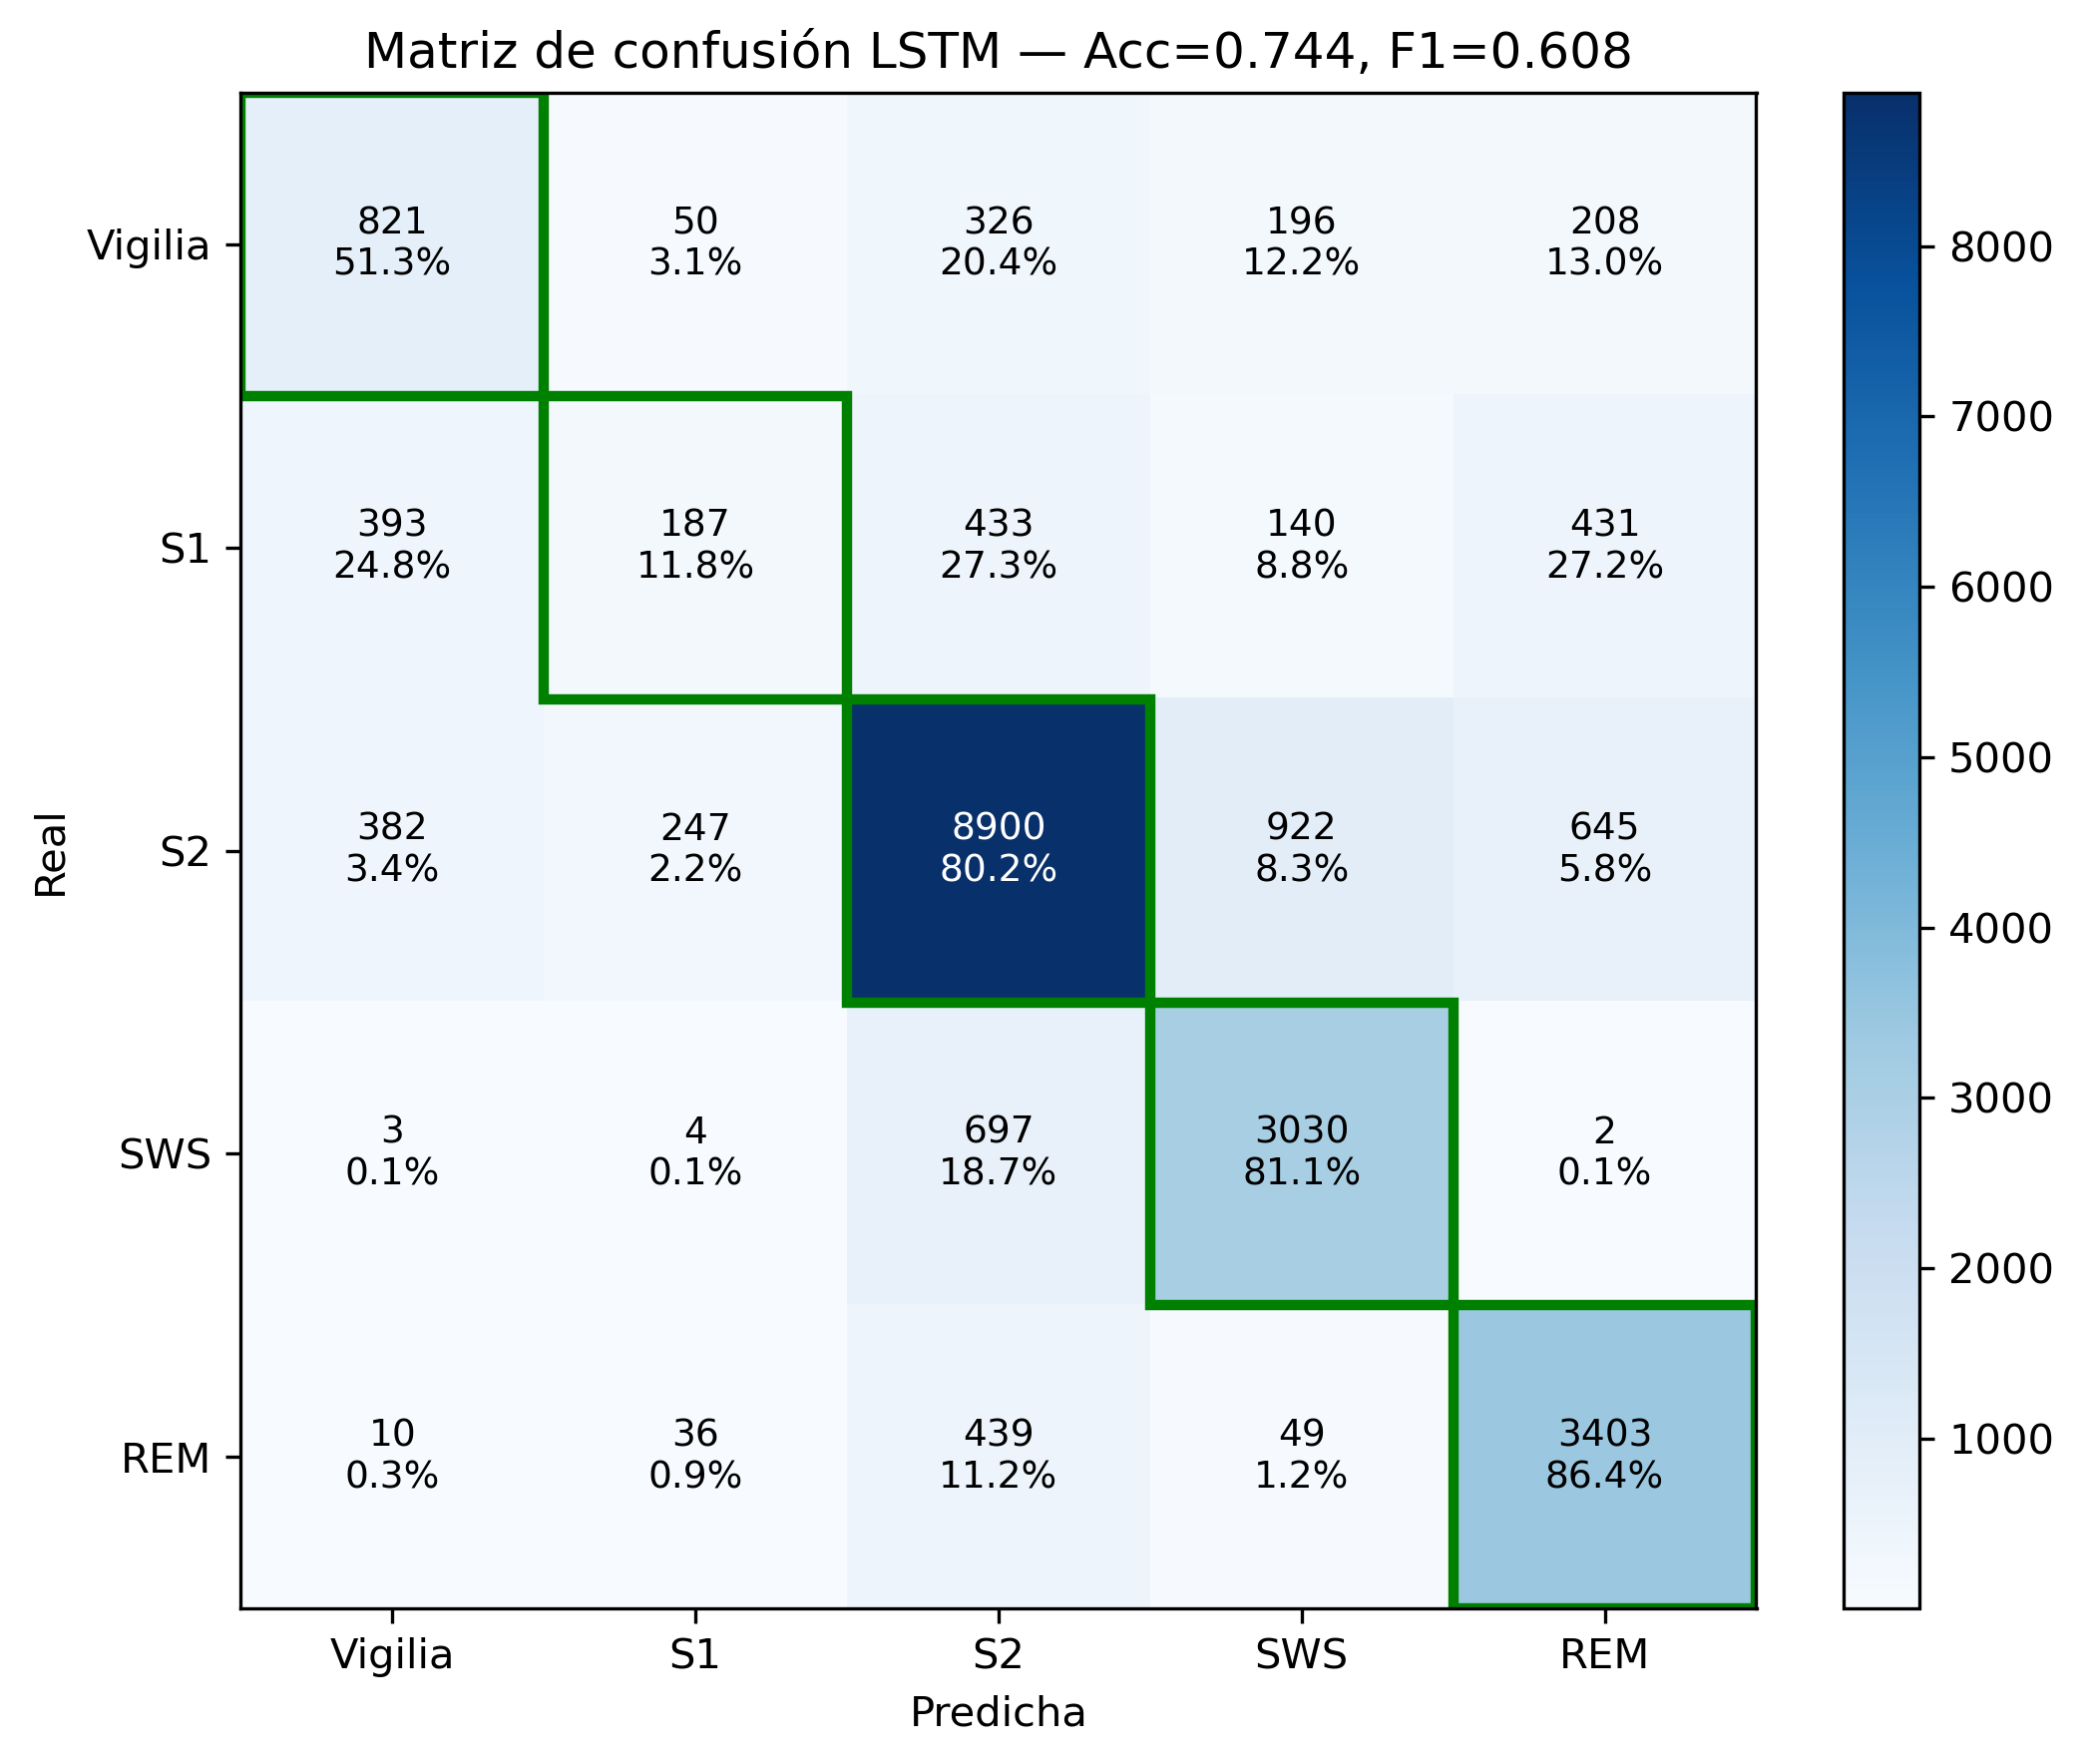
\includegraphics[width=0.8\textwidth]{confusion_real.png}
    \caption{Matriz de confusión de la LSTM (datos reales). El modelo concentra los aciertos en las fases dominantes y reparte sus errores principalmente entre fases contiguas.}
    \label{fig:confusion_lstm}
\end{figure}

\textbf{Hallazgo honesto:} En exactitud global, la LSTM (0.744) \textit{no supera} a la persistencia ni a Markov (ambos 0.880). Conviene aclarar por qué ambas líneas base arrojan cifras \textit{idénticas}: dado que en toda fila de la matriz de transición la mayor probabilidad corresponde a la diagonal (todas las $P(i|i)>0.5$, Tabla \ref{tab:diagonal_global}), el estado más probable según Markov de orden 1 es siempre el estado actual. Es decir, Markov de orden 1 \textbf{colapsa exactamente en la persistencia}; no son dos baselines independientes sino el mismo predictor por construcción. Esta coincidencia no es una deficiencia, sino una consecuencia directa de la altísima inercia del sueño: como la fase casi siempre se mantiene, ``repetir la fase anterior'' es difícil de batir en exactitud bruta. La diferencia decisiva aparece en las \textbf{transiciones}: en los instantes de cambio de fase, ambas aciertan el 0\% (por construcción, nunca predicen el cambio), mientras que la LSTM alcanza una exactitud de transición de 0.288 y un F1 de 0.238. La LSTM aporta justamente lo que las líneas base no pueden: anticipar los puntos de cambio.

La versión \textbf{subrogada} de la LSTM (entrenada y evaluada sobre secuencias permutadas dentro de cada paciente) cae a 0.262 de exactitud. Nótese que este valor queda \textit{por debajo} de la clase mayoritaria (predecir siempre S2 daría $\approx$0.48): al destruir el orden temporal, el modelo pierde toda capacidad de aprovechar la persistencia y no se limita a predecir la fase más frecuente. Esto indica que el desempeño del modelo real proviene de la estructura temporal y no de las frecuencias marginales de las fases.

\subsection{Anticipación de Transiciones: Bifurcación Pre-Cambio}

Para verificar si la LSTM \textit{anticipa} las transiciones, analizamos la probabilidad que asigna al estado destino en las 15 épocas previas a una transición real hacia REM o SWS, contrastándola con un control barajado. La Figura \ref{fig:lstm_banda} muestra esta evolución frente a las 50 redes barajadas.

\begin{figure}[htbp]
    \centering
    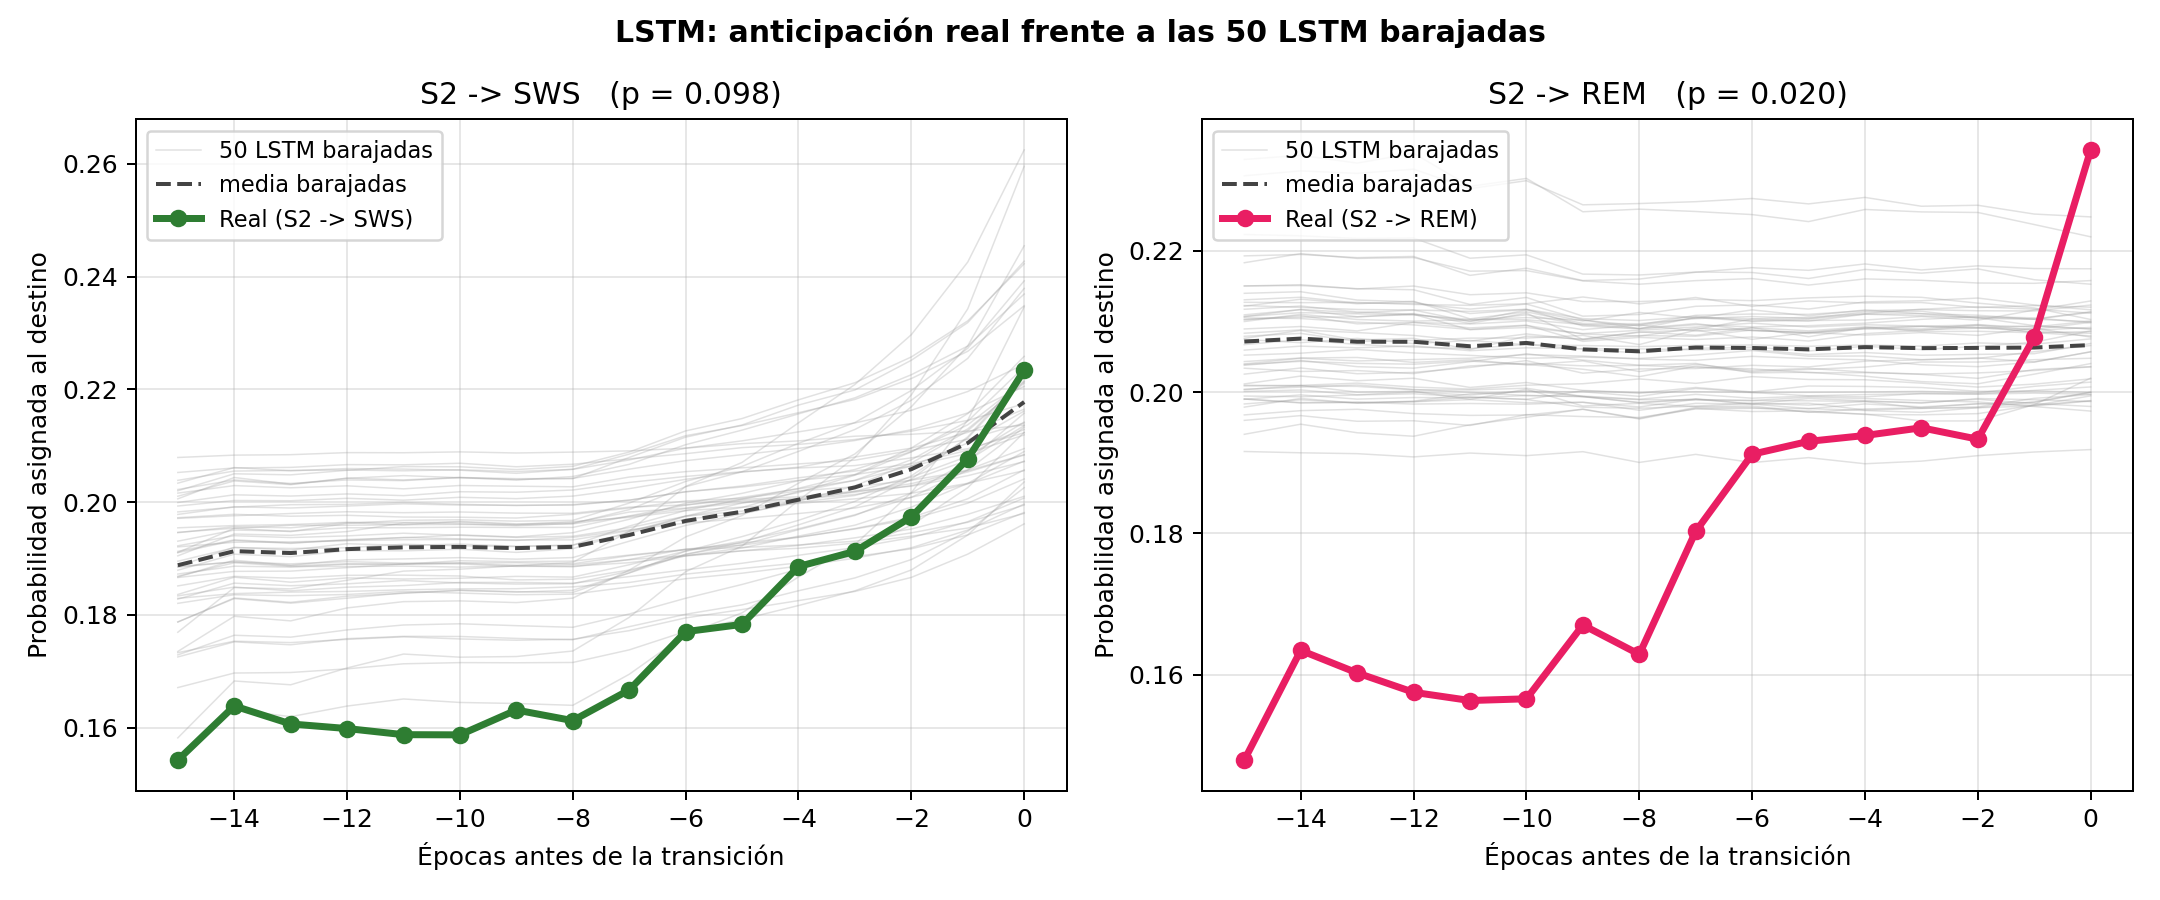
\includegraphics[width=0.95\textwidth]{lstm_bifurcacion_banda.png}
    \caption{Probabilidad que la LSTM asigna al estado destino en las 15 épocas previas a la transición, para la red entrenada con datos \textbf{reales} (línea de color) y para las \textbf{50 redes barajadas} (curvas grises tenues; su media en trazo discontinuo). Hacia \textbf{REM} (derecha) la trayectoria real se despega por encima de \textit{todas} las barajadas al acercarse al cambio ($t=0$); hacia \textbf{SWS} (izquierda) se mantiene dentro de la nube barajada, en coherencia con el resultado marginal de la prueba de permutación.}
    \label{fig:lstm_banda}
\end{figure}

En los datos \textbf{reales}, la probabilidad que la LSTM asigna al destino crece de forma sostenida al aproximarse la transición:
\begin{itemize}
    \item \textbf{Hacia REM:} de 0.148 (15 épocas antes) a 0.234 en el instante de la transición, un incremento de +0.086.
    \item \textbf{Hacia SWS:} de 0.154 a 0.223, un incremento de +0.069.
\end{itemize}

En el control \textbf{barajado}, en cambio, la trayectoria hacia REM permanece esencialmente plana y las curvas reales se despegan de la nube de las 50 redes barajadas (de forma nítida hacia REM). La LSTM, por tanto, ``siente'' la aproximación de una transición varios minutos antes de que ocurra; el siguiente apartado cuantifica si esa separación es estadísticamente significativa.

\subsection{Significancia de la Anticipación: Prueba de Permutación}

El control de la Figura \ref{fig:lstm_banda} usa las \textbf{50 LSTM barajadas} ---cada una con una permutación intra-paciente distinta y un reentrenamiento independiente--- como distribución nula de la \textbf{pendiente anticipatoria} (el incremento de la probabilidad del destino entre 15 épocas antes de la transición y el instante del cambio). Hacia \textbf{REM}, ese nulo se concentra en torno a cero (media $-0.001$, desviación estándar $0.003$) y ninguna de las 50 redes barajadas reproduce la pendiente del modelo real, con un $p$-valor empírico de $\mathbf{0.02}$: el orden temporal aporta información genuina. Hacia \textbf{SWS}, en cambio, el nulo no está centrado en cero sino desplazado hacia pendientes positivas (media $+0.029$), huella del \textit{artefacto de composición de ventana} ---al acercarse la transición, el contexto tiende a ser S2 puro, lo que altera la probabilidad incluso sin orden temporal---; aunque la pendiente real lo supera, el resultado es solo \textbf{marginal} ($p=0.10$). En conjunto, la prueba de permutación \textbf{confirma con rigor la anticipación hacia REM} y obliga a la \textbf{prudencia con SWS}, donde la señal no se separa limpiamente del artefacto geométrico.

En conjunto, la red recurrente constituye la prueba más directa de la Hipótesis H3: a diferencia de las líneas base ---que nunca anticipan un cambio--- y del deslizador puramente geométrico, la LSTM aprovecha la historia temporal para asignar una probabilidad creciente al estado destino en los minutos previos a una transición real, una señal que se desvanece al permutar la secuencia y que, hacia REM, resulta estadísticamente significativa frente a 50 redes barajadas ($p=0.02$). La Fase 2 emerge así no como un estado de relleno homogéneo, sino como un \textit{hub} dinámico cuya salida queda condicionada por su destino con varios minutos de antelación. Con ello, el recorrido de este capítulo ---de la estructura markoviana basal a la anticipación predictiva del modelo recurrente--- completa la caracterización de la dinámica del sueño sano que motivó esta tesis.

\chapter{Discusión y Conclusiones}
\chaptermark{Conclusiones}
\label{conclusiones}

La presente investigación partió de una hipótesis de trabajo: si el sueño posee una estructura secuencial no aleatoria, entonces las técnicas de Procesamiento de Lenguaje Natural (NLP) deberían ser capaces de captar parte de su ``sintaxis''. Los resultados obtenidos son consistentes con esta hipótesis y ofrecen una perspectiva complementaria sobre la función dinámica de la Fase 2 (S2), matizando su concepción tradicional como un estado de transición pasiva.

\section{Discusión de Hallazgos}

\subsection{La Fase 2 como Hub Dinámico}

Tradicionalmente, la estadificación visual (Rechtschaffen \& Kales) trata a la Fase 2 como un estado homogéneo, un ``relleno'' entre los estados fisiológicamente interesantes (SWS y REM). Sin embargo, nuestros hallazgos topológicos (Sección 4.3) y estocásticos (Sección 4.1) son consistentes con que S2 actúa como un \textbf{nodo central (hub) de la arquitectura del sueño}.

La evidencia es convergente desde múltiples perspectivas:
\begin{enumerate}
    \item \textbf{Evidencia Markoviana:} El análisis de transiciones confirmó que S2 es la ``puerta de entrada'' obligatoria al sueño profundo ($P(\text{SWS} \to \text{S2}) = 0.896$), y el único estado con acceso directo tanto a SWS como a REM.
    
    \item \textbf{Evidencia Topológica:} En el espacio latente, S2 es el único estado de sueño consolidado con similitud coseno positiva hacia el SWS ($+$0.302), manteniendo a la vez una dirección diferenciada respecto al REM ($-$0.248) y opuesta a la vigilia ($-$0.719). Sin S2, el sistema NREM perdería su nexo de continuidad.
    
    \item \textbf{Evidencia Dinámica:} Las trayectorias geométricas hacia REM y hacia SWS son distinguibles, y el modelo recurrente asigna probabilidad creciente al destino antes de la transición, lo que sugiere que la salida de S2 no es indiferente a su destino.
\end{enumerate}

Una interpretación posible ---que va más allá de lo estrictamente medido--- es que la Fase 2 funcione como un estado de \textit{negociación homeostática}, en el que el sistema ``decide'' si profundizar (ir a SWS) o activarse (ir a REM/Vigilia). Conviene subrayar que esta lectura es una hipótesis fisiológica sugerida por los datos sobre etiquetas, no una observación directa sobre el cerebro.

\subsection{La Gramática del Sueño: una Escala Justificada}

Un aporte metodológico crucial fue la determinación de la escala temporal de análisis. En lugar de descansar en un único criterio, la elección de $N=6$ (3 minutos) emergió de un \textbf{criterio multi-objetivo} que pondera tres medidas independientes evaluadas sobre toda la cohorte:

\begin{itemize}
    \item El \textbf{ajuste a la ley de Zipf} (proximidad del exponente al valor de referencia $\beta=1$).
    \item La \textbf{calidad de ese ajuste} ($R^2 = 0.977$ en $N=6$, el mejor del barrido).
    \item La \textbf{cobertura} de los bloques continuos de Fase 2 (47.33\% del tiempo en S2 con ventana de 6 épocas).
\end{itemize}

Ninguna métrica por sí sola es concluyente: el exponente $\beta$ más cercano a 1 se alcanza en $N=10$, pero a costa de degradar el ajuste y la cobertura. El valor $N=6$ es el que mejor concilia los tres objetivos. Intentar analizar el sueño con épocas aisladas de 30 segundos (como se hace en la práctica clínica estándar) es análogo a intentar entender un libro leyendo letras sueltas: se captura el símbolo, pero se pierde el significado del contexto.

Así, la escala $N=6$ no fue elegida arbitrariamente, sino seleccionada mediante un procedimiento reproducible y multi-criterio.

\subsection{El Modelo Anticipa la Siguiente Etiqueta}

Uno de los hallazgos más sugerentes de esta tesis es la \textbf{bifurcación de trayectorias} (Sección 4.4) y, sobre todo, su confirmación con el modelo recurrente: el modelo asigna una probabilidad creciente al estado destino en los pasos previos a la transición, es decir, anticipa la siguiente \textit{etiqueta} del hipnograma antes de que el cambio sea clínicamente visible. Importa precisar que esta anticipación se mide sobre la secuencia de etiquetas (épocas de 30 s), no sobre la señal EEG cruda.

La geometría del deslizador muestra además una asimetría descriptiva entre ambas transiciones:

\begin{itemize}
    \item \textbf{Mayor conservación global de la huella de origen en REM:} La similitud acumulada con el estado de partida es mayor en la trayectoria a REM (AUC = 2.574) que en la trayectoria a SWS (AUC = 1.946), lo que sugiere que el viraje a REM conserva más rasgos del contexto previo de S2 a lo largo de la ventana.
\end{itemize}

Conviene subrayar que esta asimetría procede de la \textit{misma} geometría del deslizador que \textbf{no alcanzó significancia estadística} (Sección \ref{sec:deslizador_stride}): se reporta, por tanto, como una observación \textbf{ilustrativa} y no como un hallazgo establecido.

Es notable que el modelo Word2Vec, \textbf{sin recibir ninguna instrucción explícita sobre fisiología}, aprendió automáticamente que:
\begin{itemize}
    \item REM es ortogonal a NREM (similitud negativa).
    \item S2 y SWS son variantes del mismo macro-estado.
    \item La Vigilia y S1 forman un cluster de fragmentación, separado del sueño consolidado.
\end{itemize}

Que estas relaciones surjan \textbf{sin supervisión fisiológica explícita} sugiere que la estructura del sueño está codificada en la secuencia temporal con suficiente fuerza como para que un algoritmo sensible al contexto la recupere. En otras palabras, el modelo reconstruye, a partir de la pura secuencialidad, parte de las regularidades que las reglas de Rechtschaffen \& Kales codifican explícitamente. Esto es consistente con la idea de que dichas regularidades no son un mero artefacto de las reglas de estadificación, sino que reflejan la organización del proceso fisiológico subyacente.

\subsection{¿Por Qué Anticiparía el Cerebro? Una Hipótesis Especulativa}

\textit{Nota: esta subsección es deliberadamente especulativa. Lo que los datos respaldan es que el modelo anticipa la siguiente etiqueta; la interpretación fisiológica que sigue es una hipótesis a contrastar, no un hallazgo de este trabajo.}

La existencia de una señal anticipatoria del orden de minutos plantea una pregunta natural: \textit{si esta antelación tuviera correlato fisiológico, ¿por qué se prepararía el sistema con tanta antelación?}

Una posibilidad es que tal anticipación cumpliera una función de \textbf{eficiencia y estabilidad}. Las transiciones de fase en sistemas complejos son metabólicamente costosas y potencialmente inestables. ``Pre-calentar'' gradualmente los circuitos neurales de REM (o ``enfriar'' hacia SWS) durante un par de minutos podría:

\begin{enumerate}
    \item \textbf{Reducir el costo metabólico:} Evitando cambios abruptos de configuración neural.
    \item \textbf{Proteger la estabilidad:} Permitiendo al sistema ``probar'' la viabilidad de la transición antes de comprometerla.
    \item \textbf{Coordinar subsistemas:} Dando tiempo a que múltiples regiones cerebrales sincronicen su preparación.
\end{enumerate}

Esta interpretación conectaría con marcos teóricos como el \textit{Predictive Coding} y el \textit{Free Energy Principle} de Friston, según los cuales el cerebro minimiza la ``sorpresa'' anticipando los estados futuros. Nuestros resultados son compatibles con que una dinámica anticipatoria de este tipo opere durante el sueño, pero no la prueban; establecerlo requeriría trabajar sobre la señal fisiológica y no solo sobre las etiquetas.

\subsection{Del Embedding Estático al Modelo Recurrente}

Para llevar la representación vectorial a un modelo predictivo explícito, se entrenó una red recurrente LSTM como modelo de lenguaje del sueño, que lee la secuencia de 6-gramas y predice la fase siguiente paso a paso. La evaluación se hizo con honestidad metodológica: en exactitud global, las líneas base triviales (Markov de orden 1 y persistencia) alcanzan 0.880 frente a 0.744 del LSTM, pero lo hacen prediciendo siempre ``no cambies'', por lo que su exactitud sobre las transiciones reales es exactamente 0.0. El LSTM es el único modelo con desempeño positivo en ese régimen difícil (exactitud en transiciones = 0.288). Más relevante aún, al desplegar el modelo sobre los pasos previos a una bifurcación, la probabilidad asignada a REM y SWS crece de forma sostenida en los datos reales ($+$0.086 hacia REM, $+$0.069 hacia SWS) y permanece esencialmente plana en los datos permutados. Una \textbf{prueba de permutación con 50 redes barajadas} (cada una con reentrenamiento independiente) confirma que la anticipación hacia \textbf{REM es estadísticamente significativa} ($p=0.02$: ninguna de las 50 redes barajadas reproduce la pendiente real), mientras que hacia \textbf{SWS} resulta solo \textbf{marginal} ($p=0.10$) por la contaminación del artefacto de composición de ventana. La anticipación reside, por tanto, en el orden temporal y no en la frecuencia marginal de las fases.

\section{Implicaciones del Estudio}

\subsection{Implicaciones Teóricas}

\begin{enumerate}
    \item \textbf{Revalorización de la Fase 2:} El modelo tradicional de R\&K (1968) está diseñado para clasificar, no para describir dinámica. Nuestro enfoque sugiere que S2 se comporta menos como un estado de relleno homogéneo y más como un ``controlador de tráfico'' del sueño.

    \item \textbf{El Sueño como Lenguaje:} La distribución de n-gramas es \textbf{compatible} con la estructura informativa de un lenguaje natural (ley de Zipf). Esto motiva explorar el arsenal de NLP (Transformers, modelos de atención) en el estudio del sueño.

    \item \textbf{Embeddings como Biomarcadores:} Mostramos que es posible entrenar modelos no supervisados que capturen parte de las regularidades fisiológicas a partir de la estructura secuencial, sin reglas expertas explícitas. Esto resulta prometedor para el descubrimiento de biomarcadores digitales.
\end{enumerate}

\subsection{Implicaciones Clínicas y Tecnológicas}

Si la \textbf{ventana de anticipación de unos minutos} observada sobre las etiquetas se confirmara y se replicara sobre la señal cruda, podría complementar a los métodos clásicos, que solo detectan el REM cuando ya ha comenzado (atonía muscular y movimientos oculares). Las siguientes aplicaciones son, por tanto, \textbf{prospectivas y especulativas}, no resultados de esta tesis; esbozan la dirección que podría tomar una línea de \textbf{Neuroestimulación de Lazo Cerrado (Closed-Loop)}:

\begin{itemize}
    \item \textbf{Potenciación de memoria:} Estimular justo antes de la transición a REM para optimizar la consolidación.
    \item \textbf{Diagnóstico de narcolepsia:} Detectar transiciones anómalas a REM desde vigilia (SOREMP) mediante el análisis de trayectorias vectoriales.
\end{itemize}

\section{Limitaciones}

Es necesario reconocer las limitaciones del presente estudio para contextualizar sus alcances:

\begin{enumerate}
    \item \textbf{Construcción sobre Sueño Sano:} El núcleo del modelo se construyó exclusivamente sobre sujetos sanos, que definen la referencia normativa. No se modeló la dinámica dentro de patologías específicas, por lo que la dinámica anticipatoria fina en trastornos como la narcolepsia o el insomnio queda por caracterizar.
    
    \item \textbf{Resolución Temporal:} Trabajamos sobre etiquetas discretas cada 30 segundos (épocas estándar). Aunque superamos esta limitación mediante n-gramas ($N=6$), el uso directo de la señal EEG cruda (sin etiquetado previo) podría ofrecer una granularidad temporal aún mayor.
    
    \item \textbf{Interpretabilidad de Dimensiones:} Aunque UMAP nos permite visualizar el espacio latente, las 32 dimensiones del embedding de 6-gramas siguen siendo una ``caja negra''. No podemos señalar qué dimensión específica codifica los grafoelementos propios de la Fase 2 ---los husos de sueño y los complejos K--- frente a las ondas delta del sueño profundo.
    
    \item \textbf{Causalidad vs. Correlación:} Demostramos que el vector contiene información predictiva, pero no podemos afirmar que el cambio vectorial \textit{cause} la transición. El vector podría estar capturando correlatos, no mecanismos.
\end{enumerate}

\section{Trabajo Futuro}

A partir de los hallazgos y limitaciones identificados, se proponen las siguientes líneas de investigación, ordenadas de mayor a menor calado científico:

\begin{itemize}
    \item \textbf{Contraste con cohortes patológicas (línea principal).} Es la extensión que convierte este trabajo descriptivo en un programa de investigación \textbf{que puede ponerse a prueba}: una hipótesis que los datos podrían confirmar o refutar. La hipótesis es concreta: si la Fase 2 pierde su heterogeneidad funcional en una patología, las métricas derivadas del modelo ---la \textbf{perplejidad} de la LSTM y la \textbf{pendiente anticipatoria} agregadas por paciente--- deberían \textit{desviarse de la norma} establecida sobre el sueño sano. Esto aporta un mecanismo (la degradación de la dinámica de salida de S2) y una métrica medible, no una mera comparación. El caso más nítido es la \textbf{Narcolepsia Tipo 1}, con su intrusión anómala de REM, y el contraste debería hacerse sobre cohortes multicéntricas de tamaño suficiente para separar la señal de enfermedad de la de procedencia. Trabajos recientes de modelos de lenguaje del hipnograma ya exploran esta dirección diagnóstica \citep{yu2024sleepgpt}, lo que refuerza la pertinencia ---y la viabilidad--- de esta línea.

    \item \textbf{Validación sobre la señal EEG cruda.} Más que una mejora de granularidad temporal, esta línea es la \textbf{prueba de que la anticipación es genuina y no un artefacto de la estadificación}. Todo el análisis se apoya en etiquetas de 30\,s que ya son una discretización humana (reglas de R\&K), por lo que un revisor podría objetar que la señal anticipatoria refleje el \textit{modo en que los expertos asignan las épocas cerca de las transiciones} y no una dinámica fisiológica subyacente. Entrenar el modelo directamente sobre segmentos de EEG ---sin estadificación previa--- es lo único que cierra esa puerta: si la pendiente anticipatoria persiste sobre la señal cruda, el hallazgo queda libre del sesgo del observador. Por eso es una prueba de validez, no solo un refinamiento.

    \item \textbf{Modelos generativos de secuencias de sueño.} El salto del embedding estático al modelo recurrente invita a continuar con arquitecturas de atención, pero este terreno \textbf{ya no es virgen}: modelos generativos del hipnograma tipo \textit{SleepGPT}/\textit{HypnoGPT} \citep{yu2024sleepgpt} y transformadores de estadificación \citep{phan2022sleeptransformer} ya tratan la secuencia de fases como un lenguaje. La aportación específica no sería ``inaugurar'' un \textit{Sleep-GPT}, sino \textbf{extender ese enfoque generativo a la tarea anticipatoria sobre \textit{embeddings} de \textit{n}-gramas}, evaluando si la \textit{Self-Attention} captura dependencias de rango largo (ciclos de $\sim$90 min) que la ventana fija de 3 minutos no alcanza.

    \item \textbf{Implementación en tiempo real.} Como ingeniería derivada de lo anterior, un prototipo ligero ejecutable en dispositivos vestibles (\textit{wearables}) que calcule la trayectoria vectorial paso a paso y prediga la fase siguiente en vivo, habilitando las aplicaciones de lazo cerrado discutidas más arriba.
\end{itemize}

\clearpage
\section{Conclusiones Finales}

Esta tesis modeló la dinámica de las transiciones del sueño mediante un enfoque híbrido estocástico-vectorial. Se cumplieron los objetivos planteados, con apoyo para las tres hipótesis de investigación ---sólido para H1 y H2, y parcial para H3:

\begin{enumerate}
    \item \textbf{H1 (Estructural):} El sueño sano no es un proceso aleatorio, sino que posee una estructura no fragmentada. El análisis de Cadenas de Markov lo respalda: las fases muestran alta inercia, las transiciones respetan la topología fisiológica (no existe el atajo SWS$\rightarrow$REM) y la estabilidad se degrada de forma ordenada a lo largo de la noche.

    \item \textbf{H2 (Lingüística):} Los hipnogramas pueden tratarse como secuencias simbólicas con propiedades análogas a las de un lenguaje. A una escala de \textbf{3 minutos ($N=6$)} ---seleccionada mediante un criterio multi-objetivo que concilia la proximidad a la ley de Zipf, la calidad del ajuste ($R^2 = 0.977$) y la cobertura de los bloques de Fase 2--- la distribución de n-gramas es compatible con la organización estadística de un idioma.

    \item \textbf{H3 (Dinámica):} La salida de la Fase 2 no es indiferente a su destino. El modelo recurrente aprende a anticipar el siguiente estado: en los minutos previos a una transición real eleva de forma sostenida la probabilidad que asigna al destino, y esa anticipación se desvanece en cuanto se rompe el orden temporal de la secuencia, lo que confirma que reside en la estructura del relato y no en la frecuencia de las fases. La señal es \textbf{sólida hacia el REM} y más tentativa hacia el sueño profundo, y su tamaño de efecto es modesto; se trata, por tanto, de un apoyo \textbf{parcial pero direccionalmente nítido} a la hipótesis. Su lectura de fondo ---que la Fase 2 no se limita a esperar la transición, sino que parece preparar su salida--- queda planteada con la prudencia que merece, y su consolidación definitiva pasa por replicarla sobre la señal EEG cruda.
\end{enumerate}

En conclusión, los resultados son consistentes con la idea de que \textbf{el sueño posee una estructura secuencial legible con herramientas de lenguaje}. Las secuencias de fases no se comportan como ruido estocástico, sino que exhiben regularidades que un modelo sensible al contexto puede aprender y, en cierta medida, anticipar. Confirmar la robustez de esta señal anticipatoria y trasladarla a la señal cruda son los pasos naturales para convertir estas observaciones en una herramienta útil para la neurociencia del sueño.


\bibliographystyle{recursos/apa_esp}
\bibliography{recursos/bibliografia_fc}

\end{document}